\subsection*{Supplementary figures}
\label{supp}

\renewcommand{\thefigure}{S\arabic{figure}}
\setcounter{figure}{0}
\begin{center}
\begin{figure}[H]
  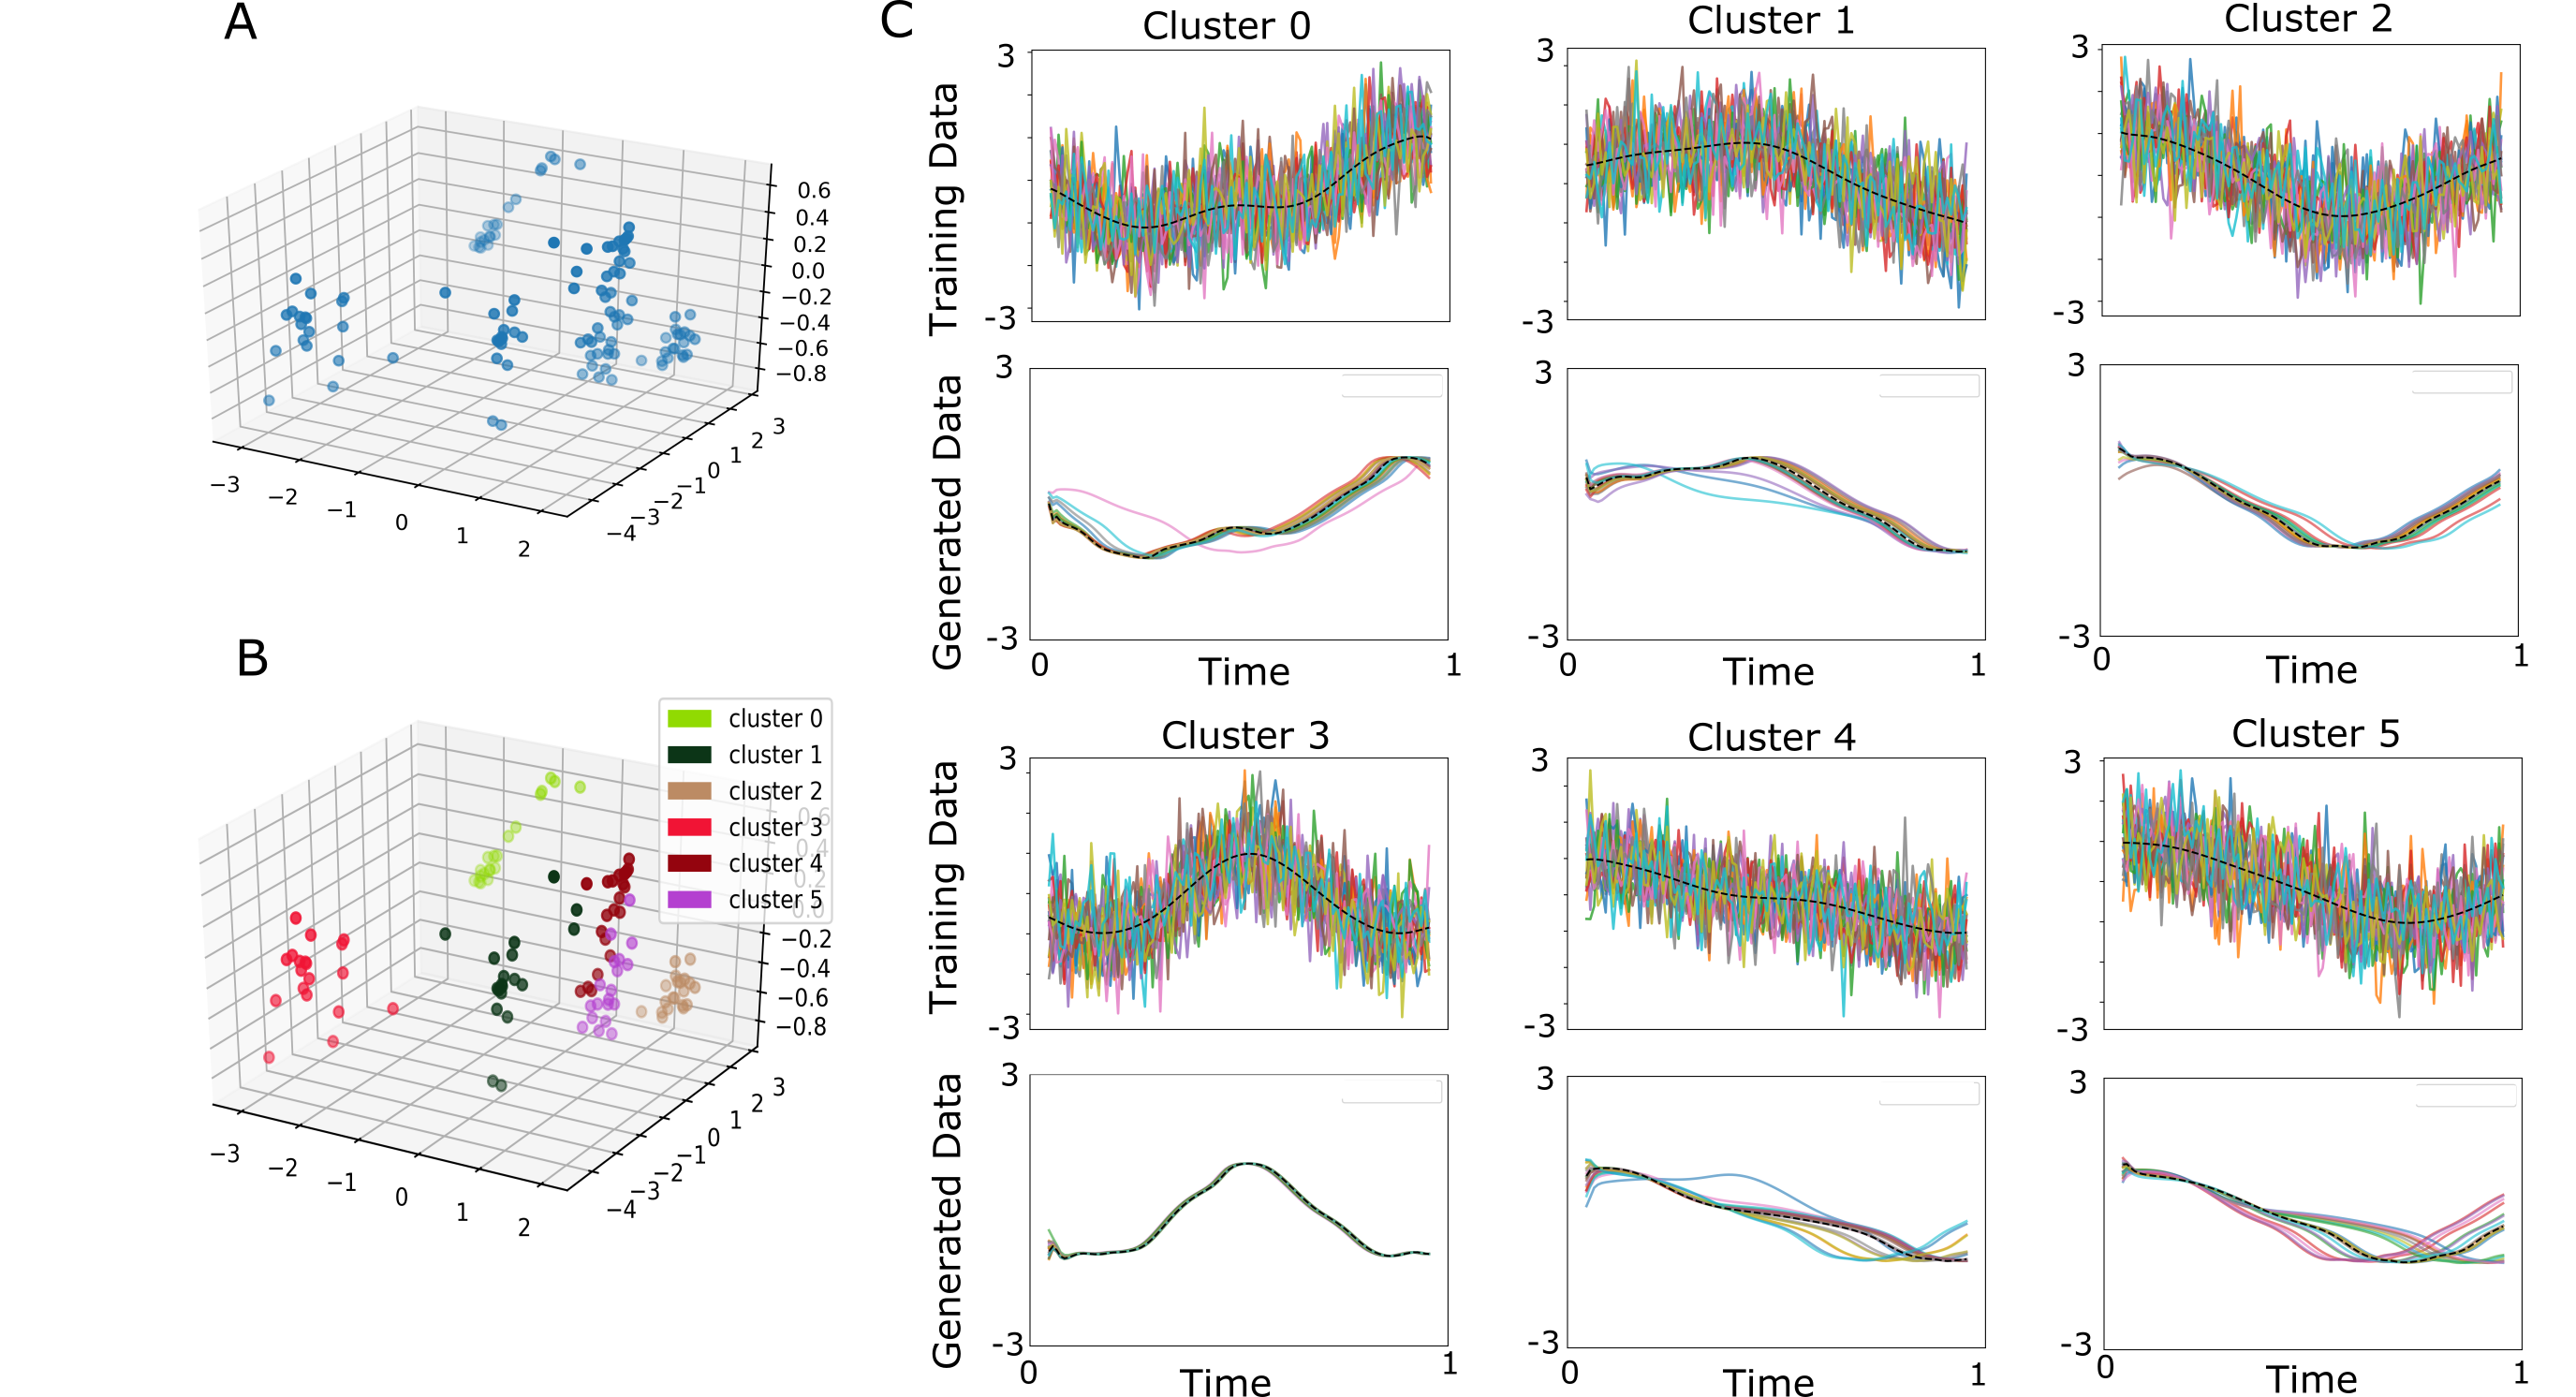
\includegraphics[width=\linewidth]{./figures/noisy_sim.png}
 % archetecture.png: 1149x508 px, 72dpi, 40.53x17.92 cm, bb=0 0 1149 508
    \caption[Demonstration of RVAgene working principle on simulated data with high noise.]{\textbf{Demonstration of RVAgene working principle on simulated data with high noise.} Gaussian noise drawn from $\cN(0,0.7)$ was added to the simulated data to produce a dataset with heavy noise. RVAgene learns the latent space shown in ({\bf A}). ({\bf B}) shows 6 clusters learned by k-means on the learned latent space. ({\bf C}) shows original training data and model generated data from random points in the latent space sampled from $\cN(\mu,0.4\bI)$ around each cluster mean $\mu$ for each of the 6 clusters detected by k-means.}
  \label{fig:figS1}
\end{figure}
\end{center}
\newpage

\begin{center}
\begin{figure}[H]
  \includegraphics[width=\linewidth]{./figures/sl_ESC_r.png}
 % archetecture.png: 1149x508 px, 72dpi, 40.53x17.92 cm, bb=0 0 1149 508
    \caption[Characterization of gene dynamics by linear fit using Pearson correlation coefficient for 5 sample genes in the ESC differentiation dataset]{Characterization of gene dynamics by linear fit using Pearson correlation coefficient for 5 sample genes in the ESC differentiation dataset  \citep{Klein2015}. Blue lines represents original data and orange lines represents linear fits. The Pearson correlation coefficient $r$ is given for each plot.}
  \label{fig:figS2}
\end{figure}
\end{center}
\newpage

\begin{center}
\centering
\begin{figure}[H]
  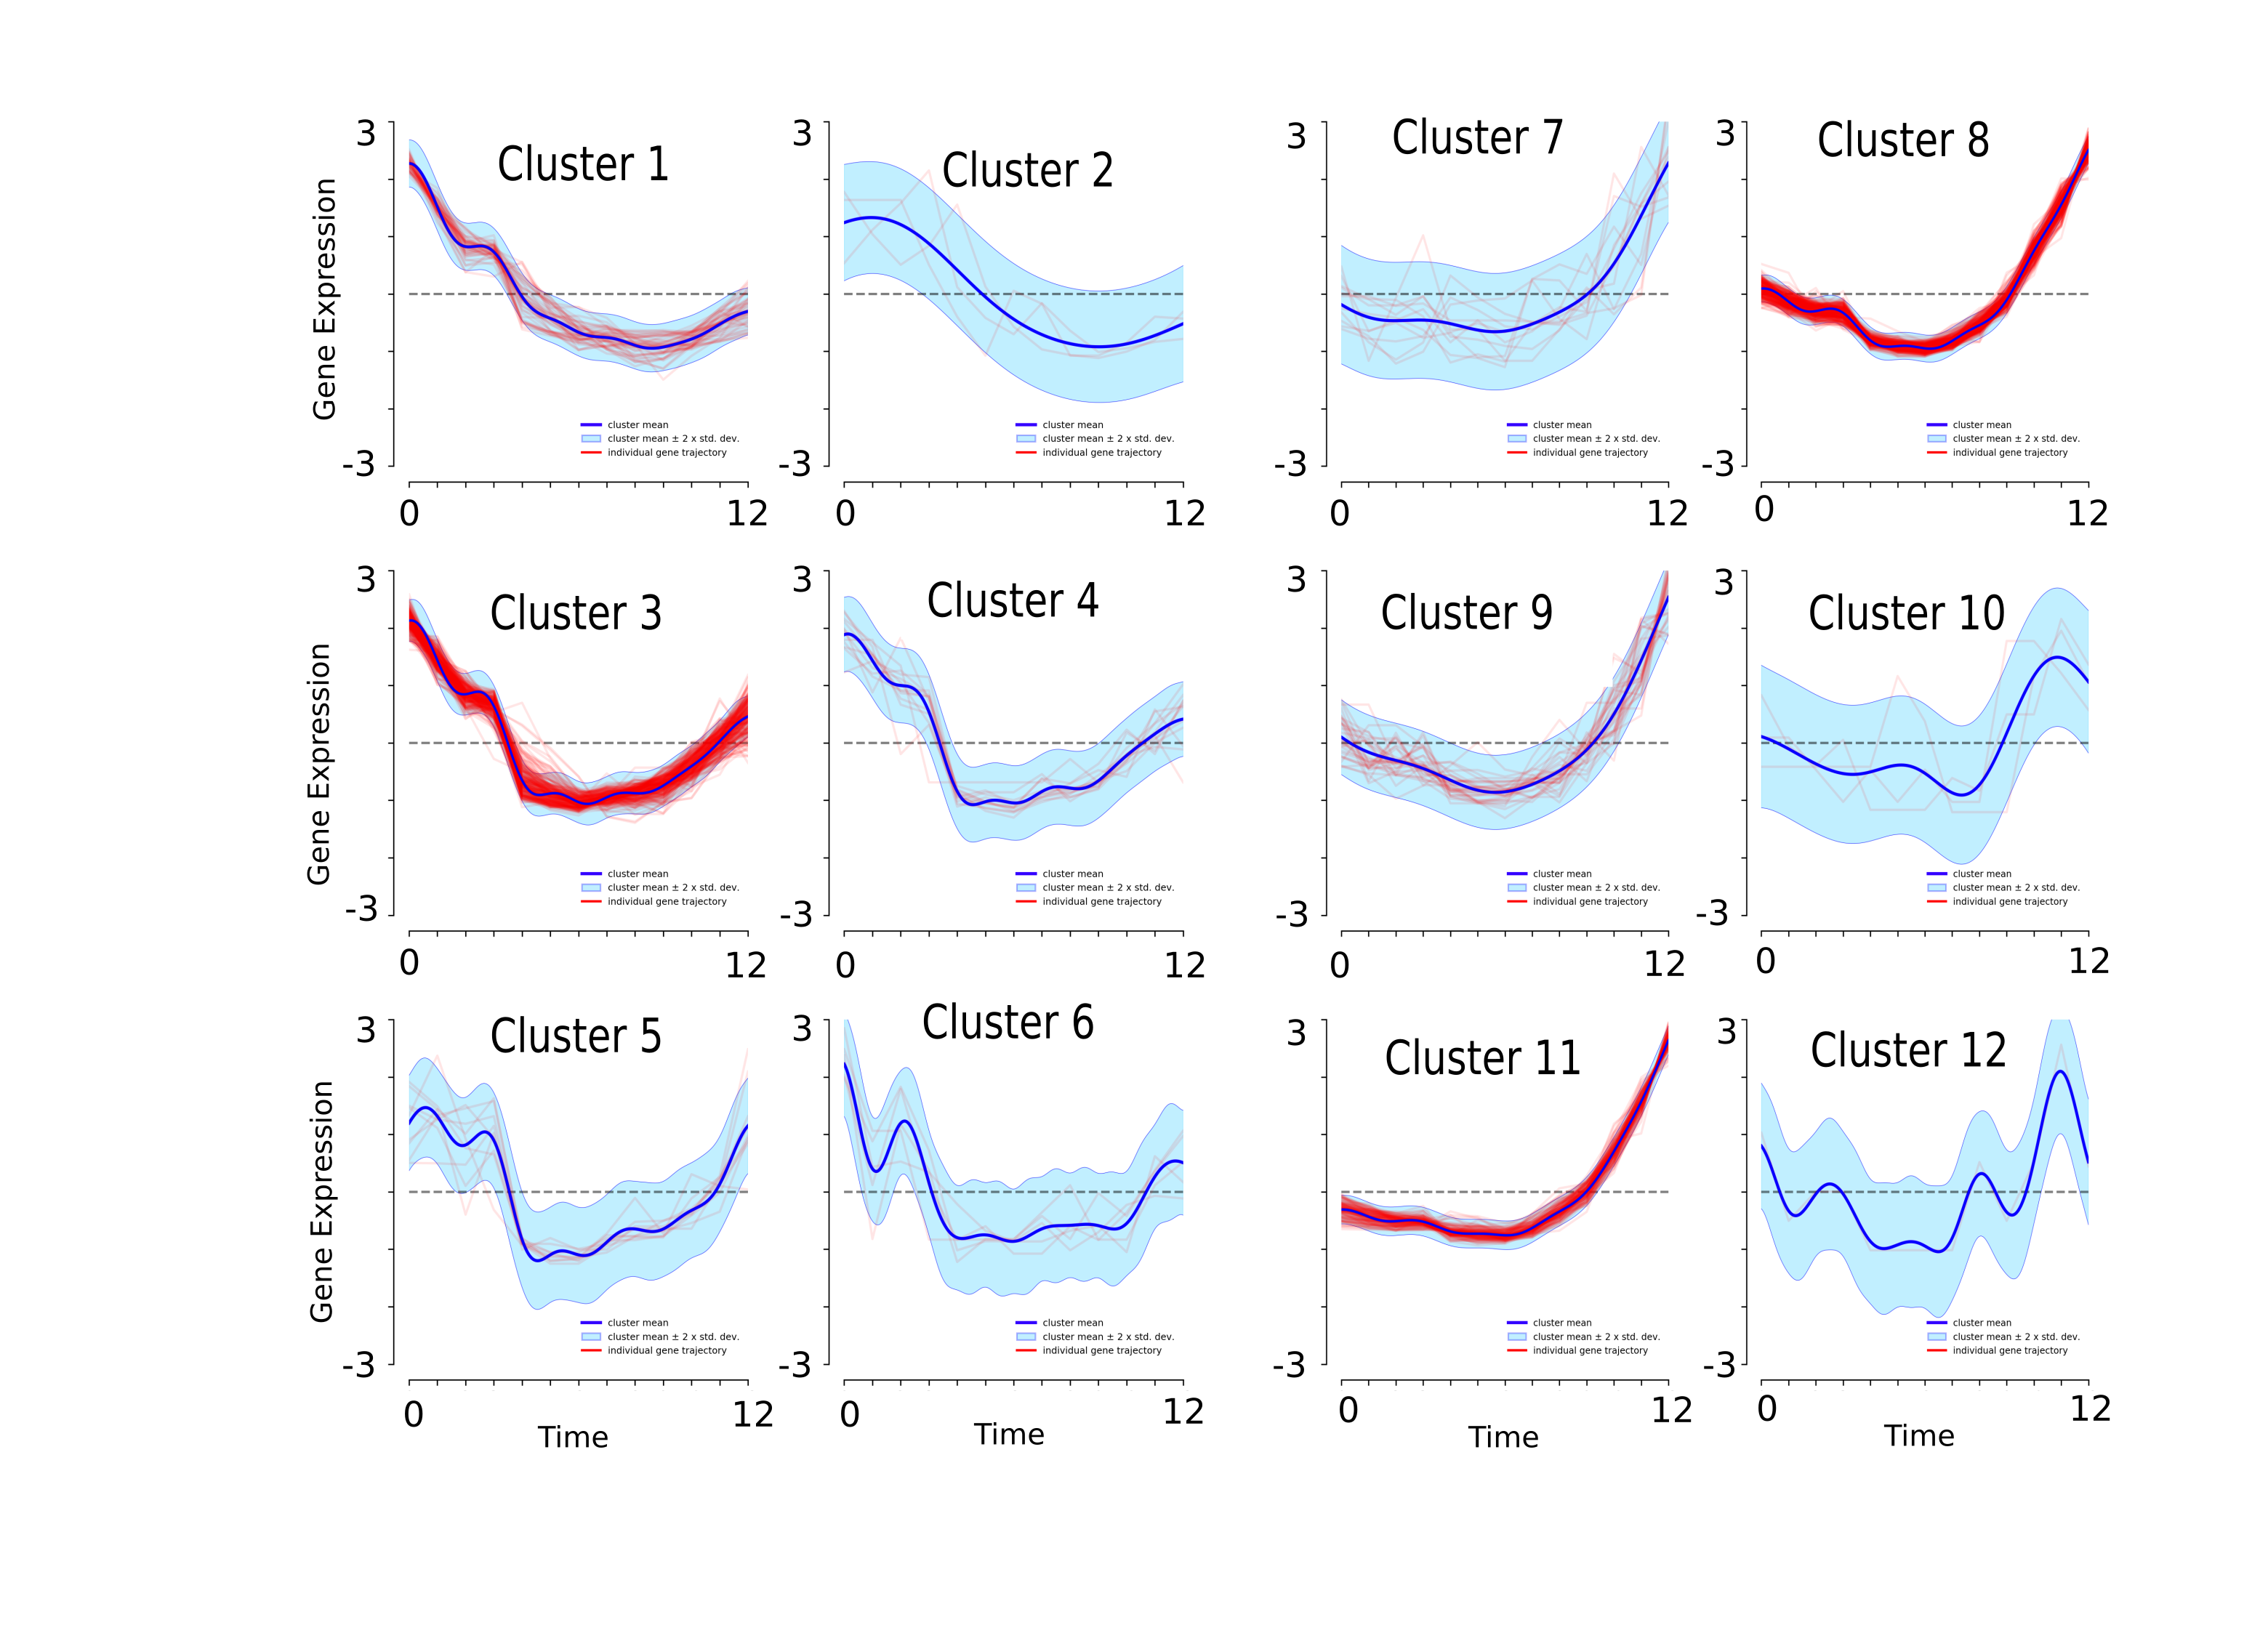
\includegraphics[width=\linewidth,height=0.4\textheight]{figures/fig4.png}
 % archetecture.png: 1149x508 px, 72dpi, 40.53x17.92 cm, bb=0 0 1149 508
    \caption[Clusters detected by the unsupervised clustering algorithm DPGP for ESC differentiation.]{\textbf{Clusters detected by the unsupervised clustering algorithm DPGP for ESC differentiation.} Clusters detected by DPGP in the ESC differentiation dataset  \citep{Klein2015} with default hyperparameters showing cluster means (black), mean $\pm$ 2 s.d. in (blue) and cluster members (red). }
   \label{fig:figS3}
\end{figure}
\end{center}
\newpage
\begin{center}
\begin{figure}
  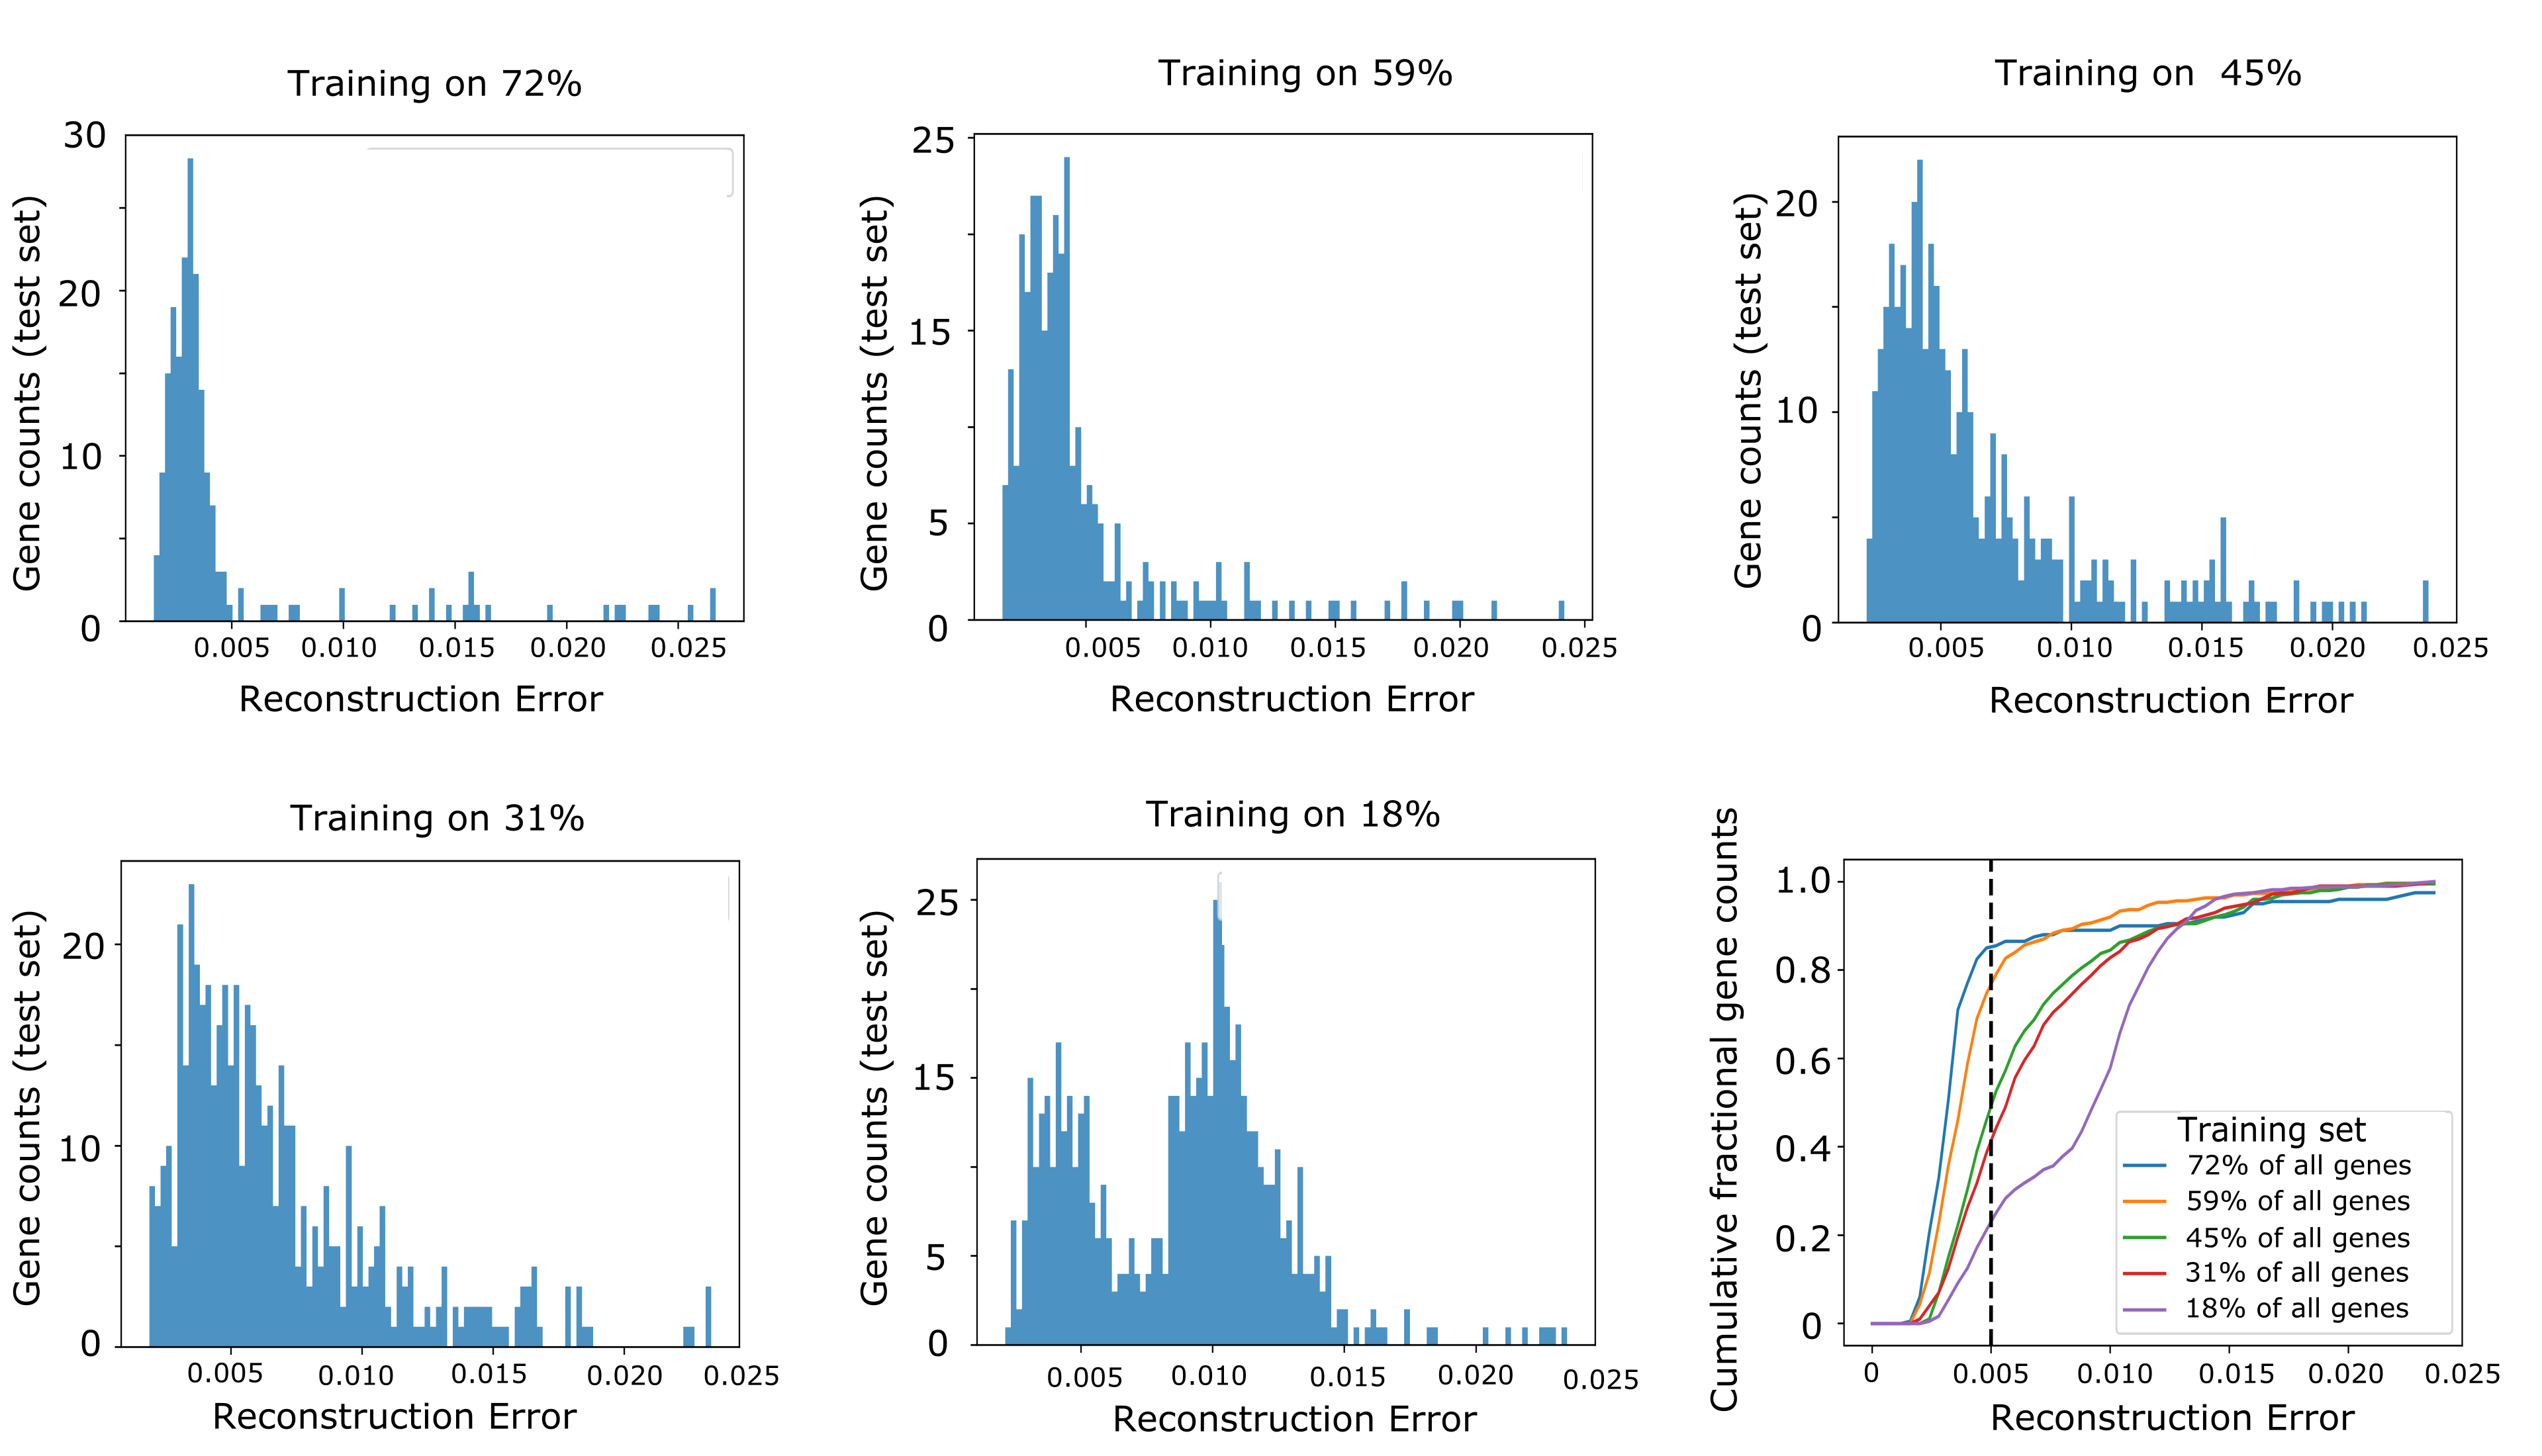
\includegraphics[width=\linewidth]{./figures/supp_varying_test_set_sizes.png}
 % archetecture.png: 1149x508 px, 72dpi, 40.53x17.92 cm, bb=0 0 1149 508
    \caption[Accuracy of RVAgene reconstructions for different train/test group sizes.]{{\bf Accuracy of RVAgene reconstructions for different train/test group sizes.} Distributions of reconstruction errors on randomly sampled sets of test genes, where the full data were split into test groups of: 200 genes (train on 72\%), 300 genes (train on 59\%), 400 genes (train on 45\%), 500 genes (train on 31\%), and 600 genes (train on 18\%). Cumulative fractional distribution of reconstruction errors (cumulative count/test set size) for all groups.}
  \label{fig:figS4}
\end{figure}
\end{center}
\newpage

\begin{center}
\begin{figure}[H]
  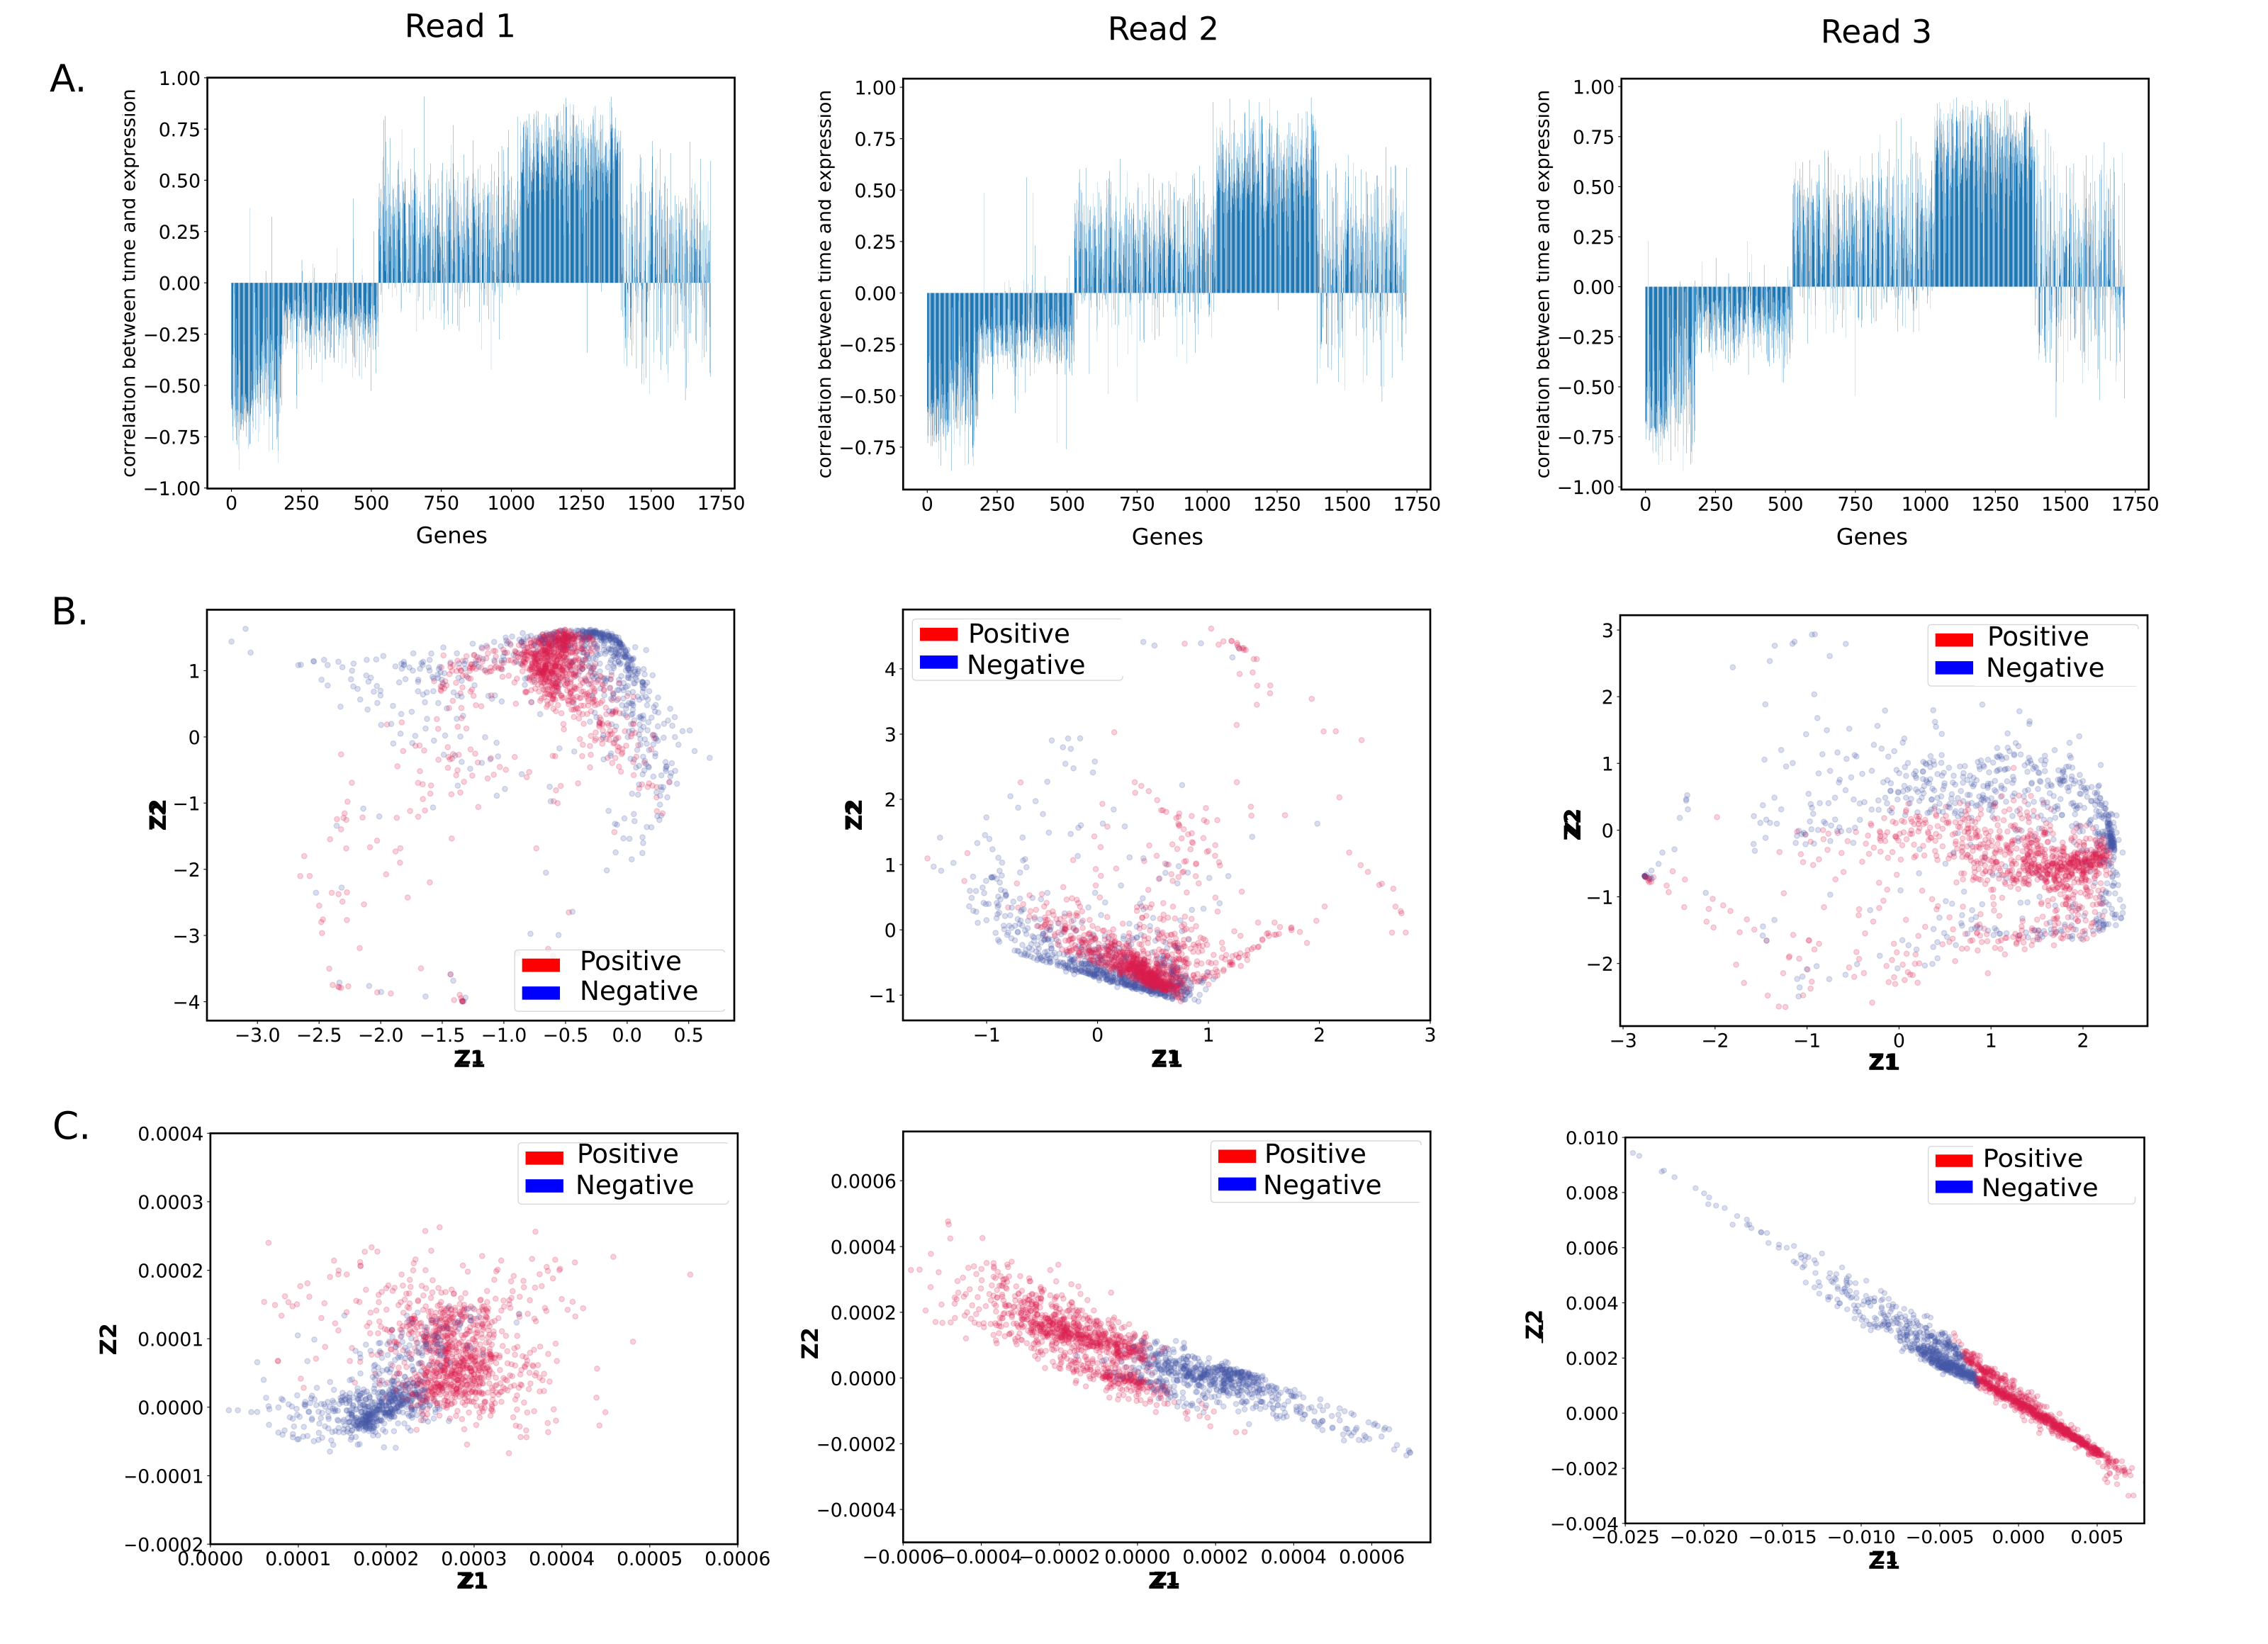
\includegraphics[width = \linewidth]{figures/fig8.png}
 % archetecture.png: 1149x508 px, 72dpi, 40.53x17.92 cm, bb=0 0 1149 508
    \caption[Modeling response to kidney injury and analysis of linear fits.]{\textbf{Modeling response to kidney injury and analysis of linear fits.}
    ({\bf A}) Pearson correlation coefficients between gene expression and time for each differentially expressed gene in the kidney injury dataset for each of the 3 replicates \citep{liu2017molecular}. ({\bf B}) RVAgene latent space representation of fitted model for each replicate; color represents positive or negative correlation coefficients. ({\bf C}) RVAgene latent space representation learnt for the same three replicates as in (B), but where every input gene was normalized  so that its expression sums to 1.}
  \label{fig:figS5}
\end{figure}
\end{center}
\newpage

\begin{center}
\begin{figure}[H]
  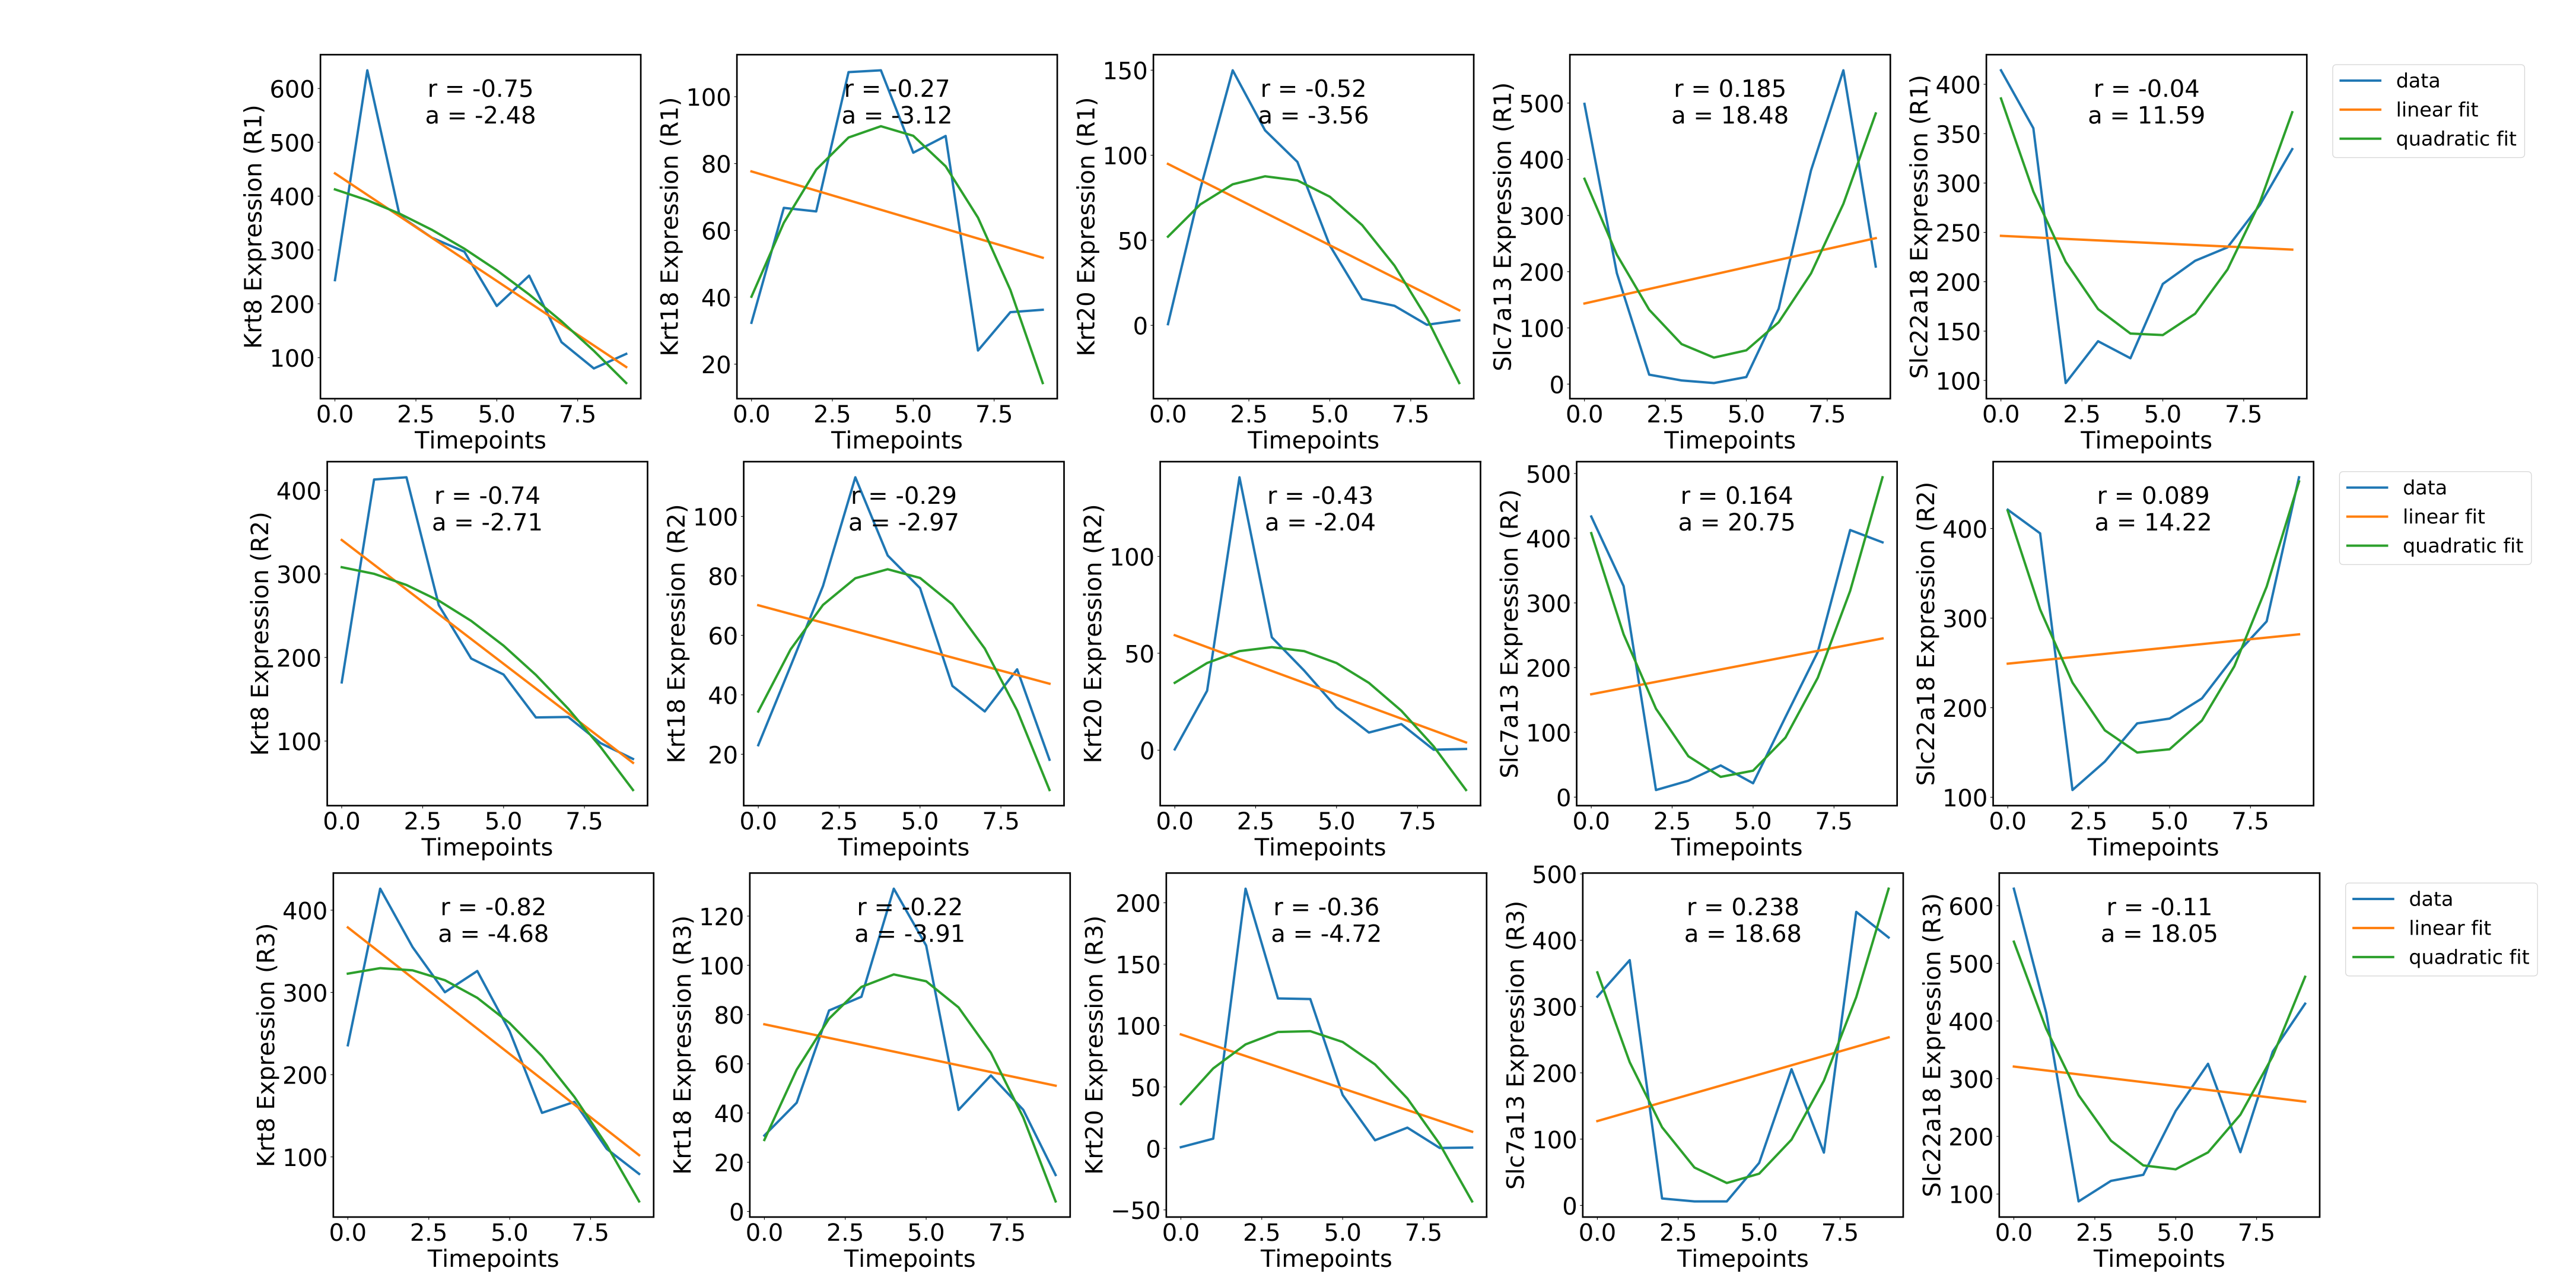
\includegraphics[width=\linewidth]{./figures/sl_JCI_r.png}
 % archetecture.png: 1149x508 px, 72dpi, 40.53x17.92 cm, bb=0 0 1149 508
    \caption[Comparison of linear and quadratic fits to describe gene dynamics in response to kidney injury.]{\textbf{Comparison of linear and quadratic fits to describe gene dynamics in response to kidney injury.}
    For each of the three replicates (R1-R3), five genes are shown, with experimental data (blue), linear fit (orange), and quadratic fit (green). 
    Pearson correlation coefficients, $r$, and quadratic coefficients, $a$ ($x = at^2 + bt + c$), are given for each plot.}
  \label{fig:figS6}
\end{figure}
\end{center}
\newpage

\begin{center}
\begin{figure}[H]
  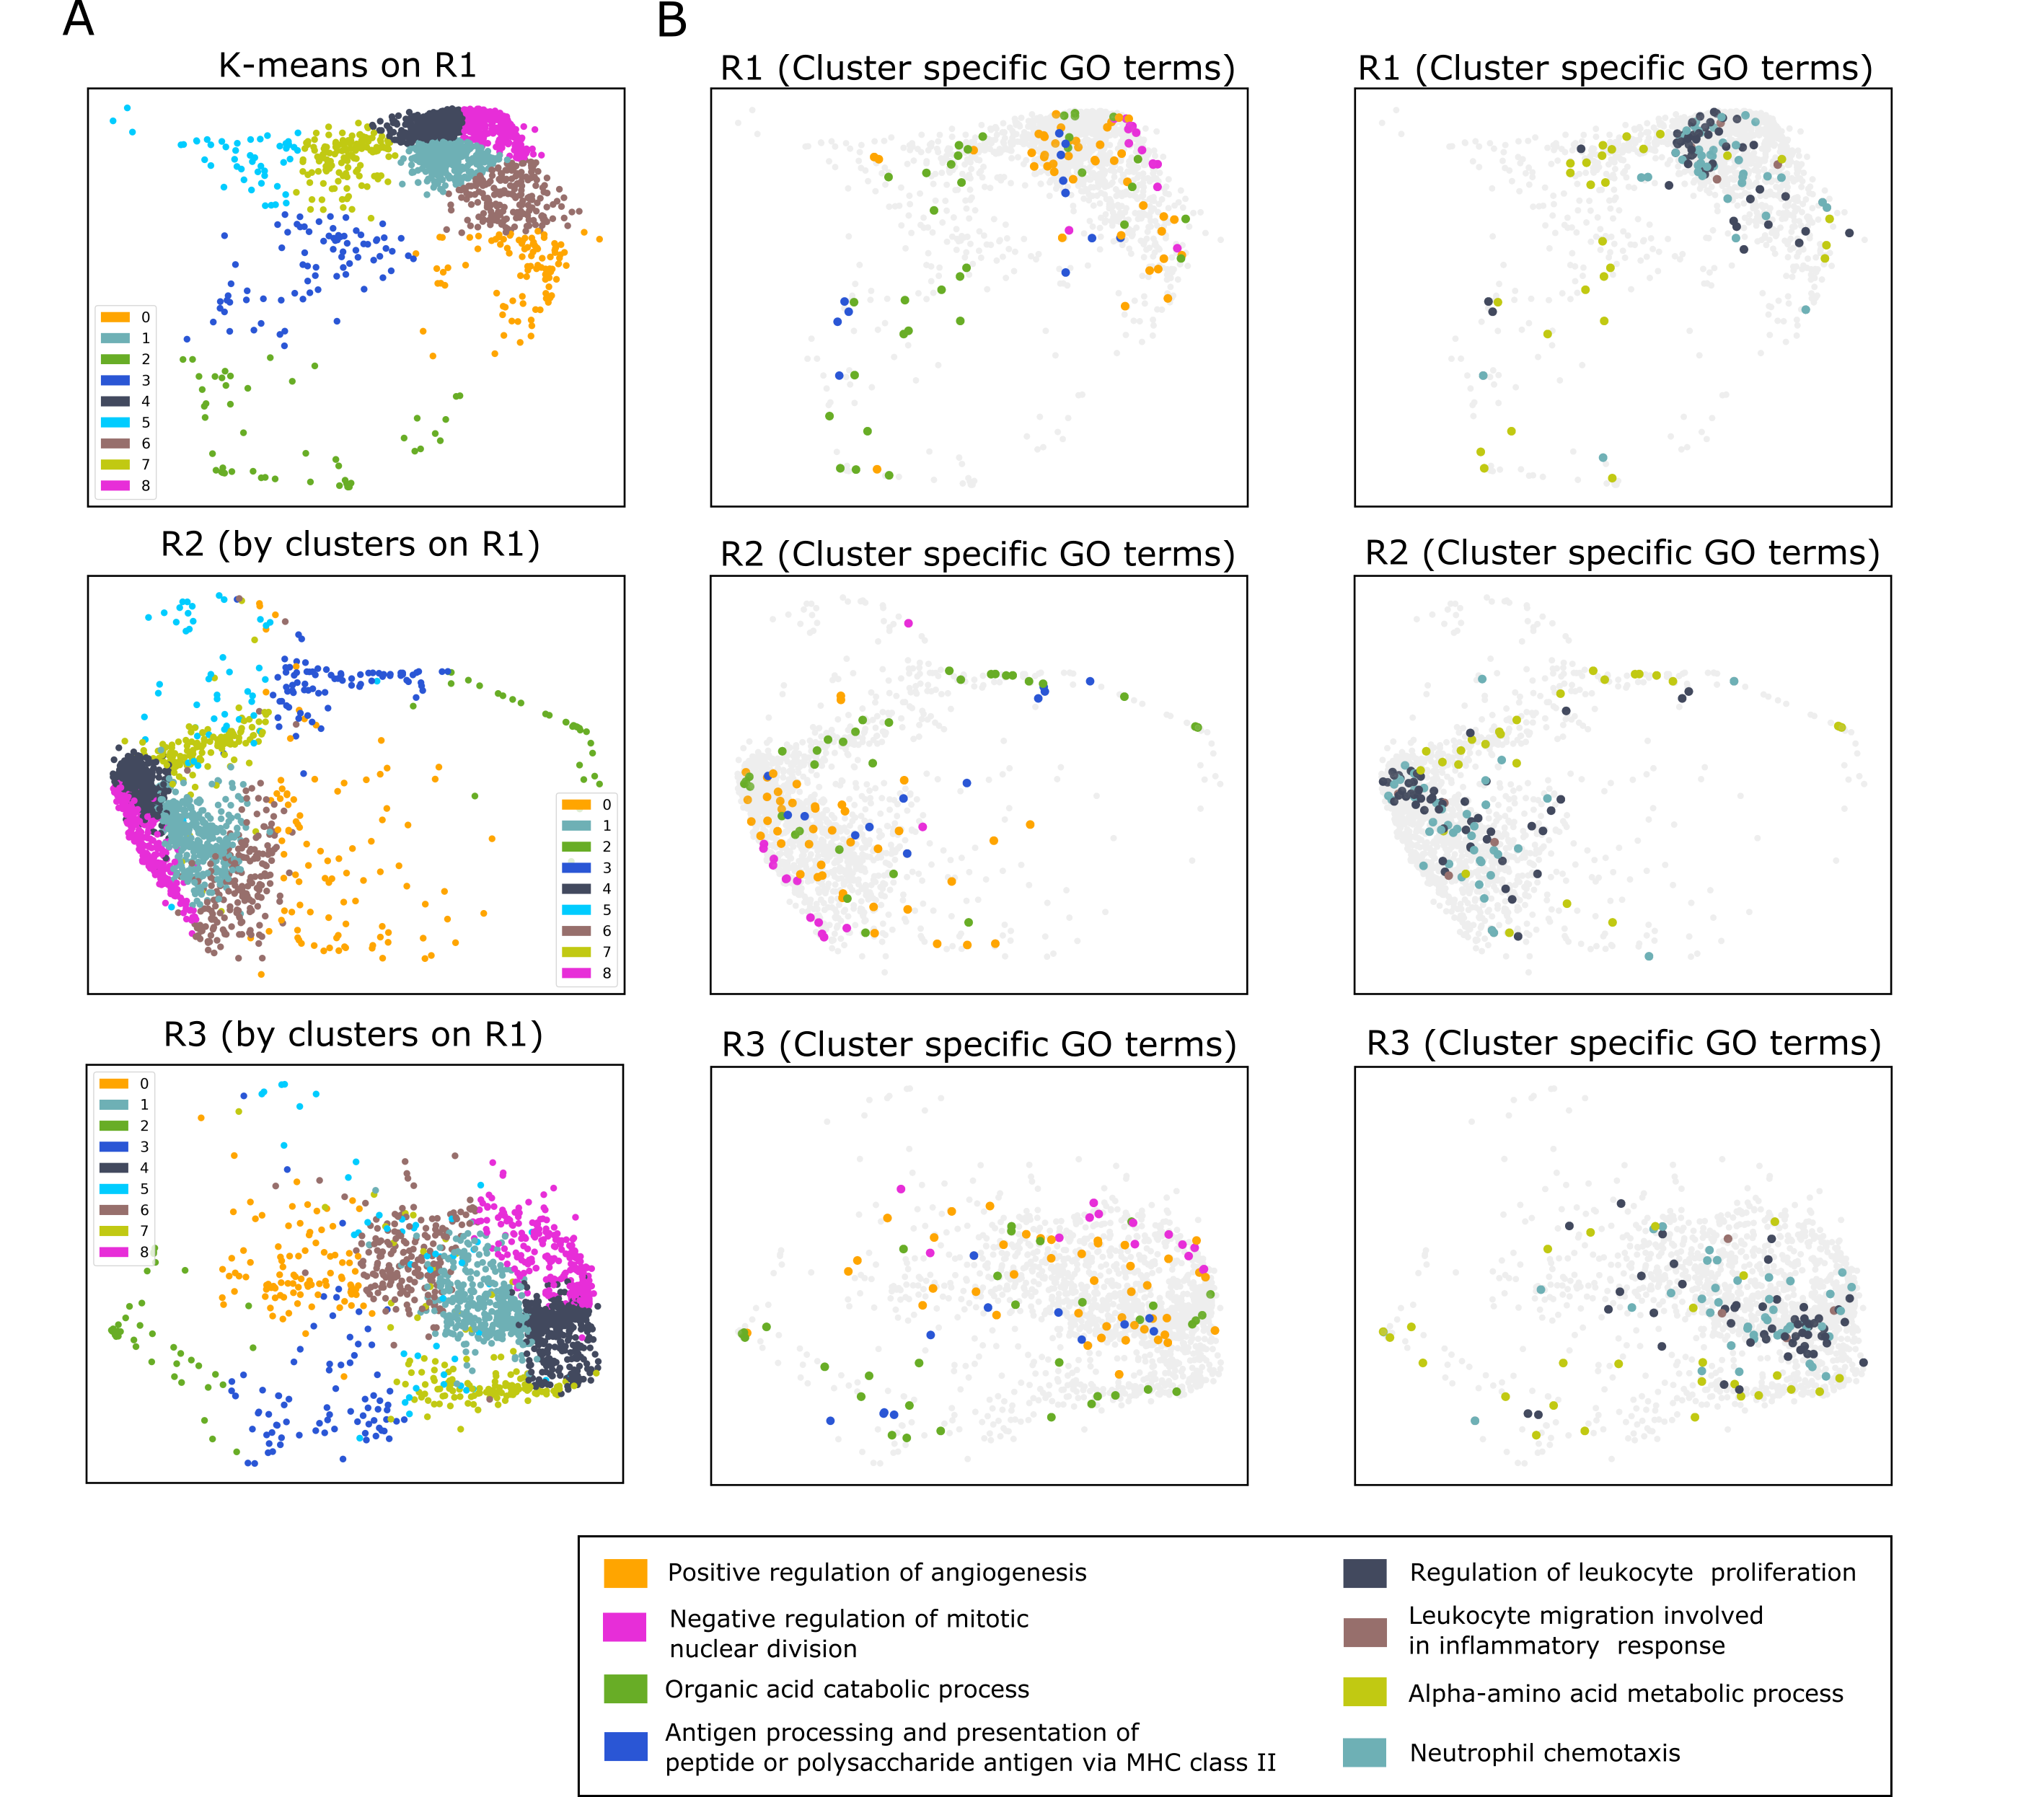
\includegraphics[width=\linewidth]{./figures/supp_go.png}
 % archetecture.png: 1149x508 px, 72dpi, 40.53x17.92 cm, bb=0 0 1149 508
    \caption[Clustering on R1 and cluster specific GO enrichment analysis.]{\textbf{Clustering on R1 and cluster specific GO enrichment analysis.} We performed k-means clustering on latent space learned by RVAgene on R1 with $k=9$. We also show learned latent space on R2 and R3 annotated by the clustering done on R1. All clusters (except cluster 5) appears well preserved. We perform GO analysis for each cluster and select one significant GO term from each cluster (except cluster 5) and show how all genes in the dataset corresponding to each GO term appears on the latent space for all three replicates. }
  \label{fig:figS8}
\end{figure}
\end{center}
\newpage

\begin{center}
\begin{figure}[H]
  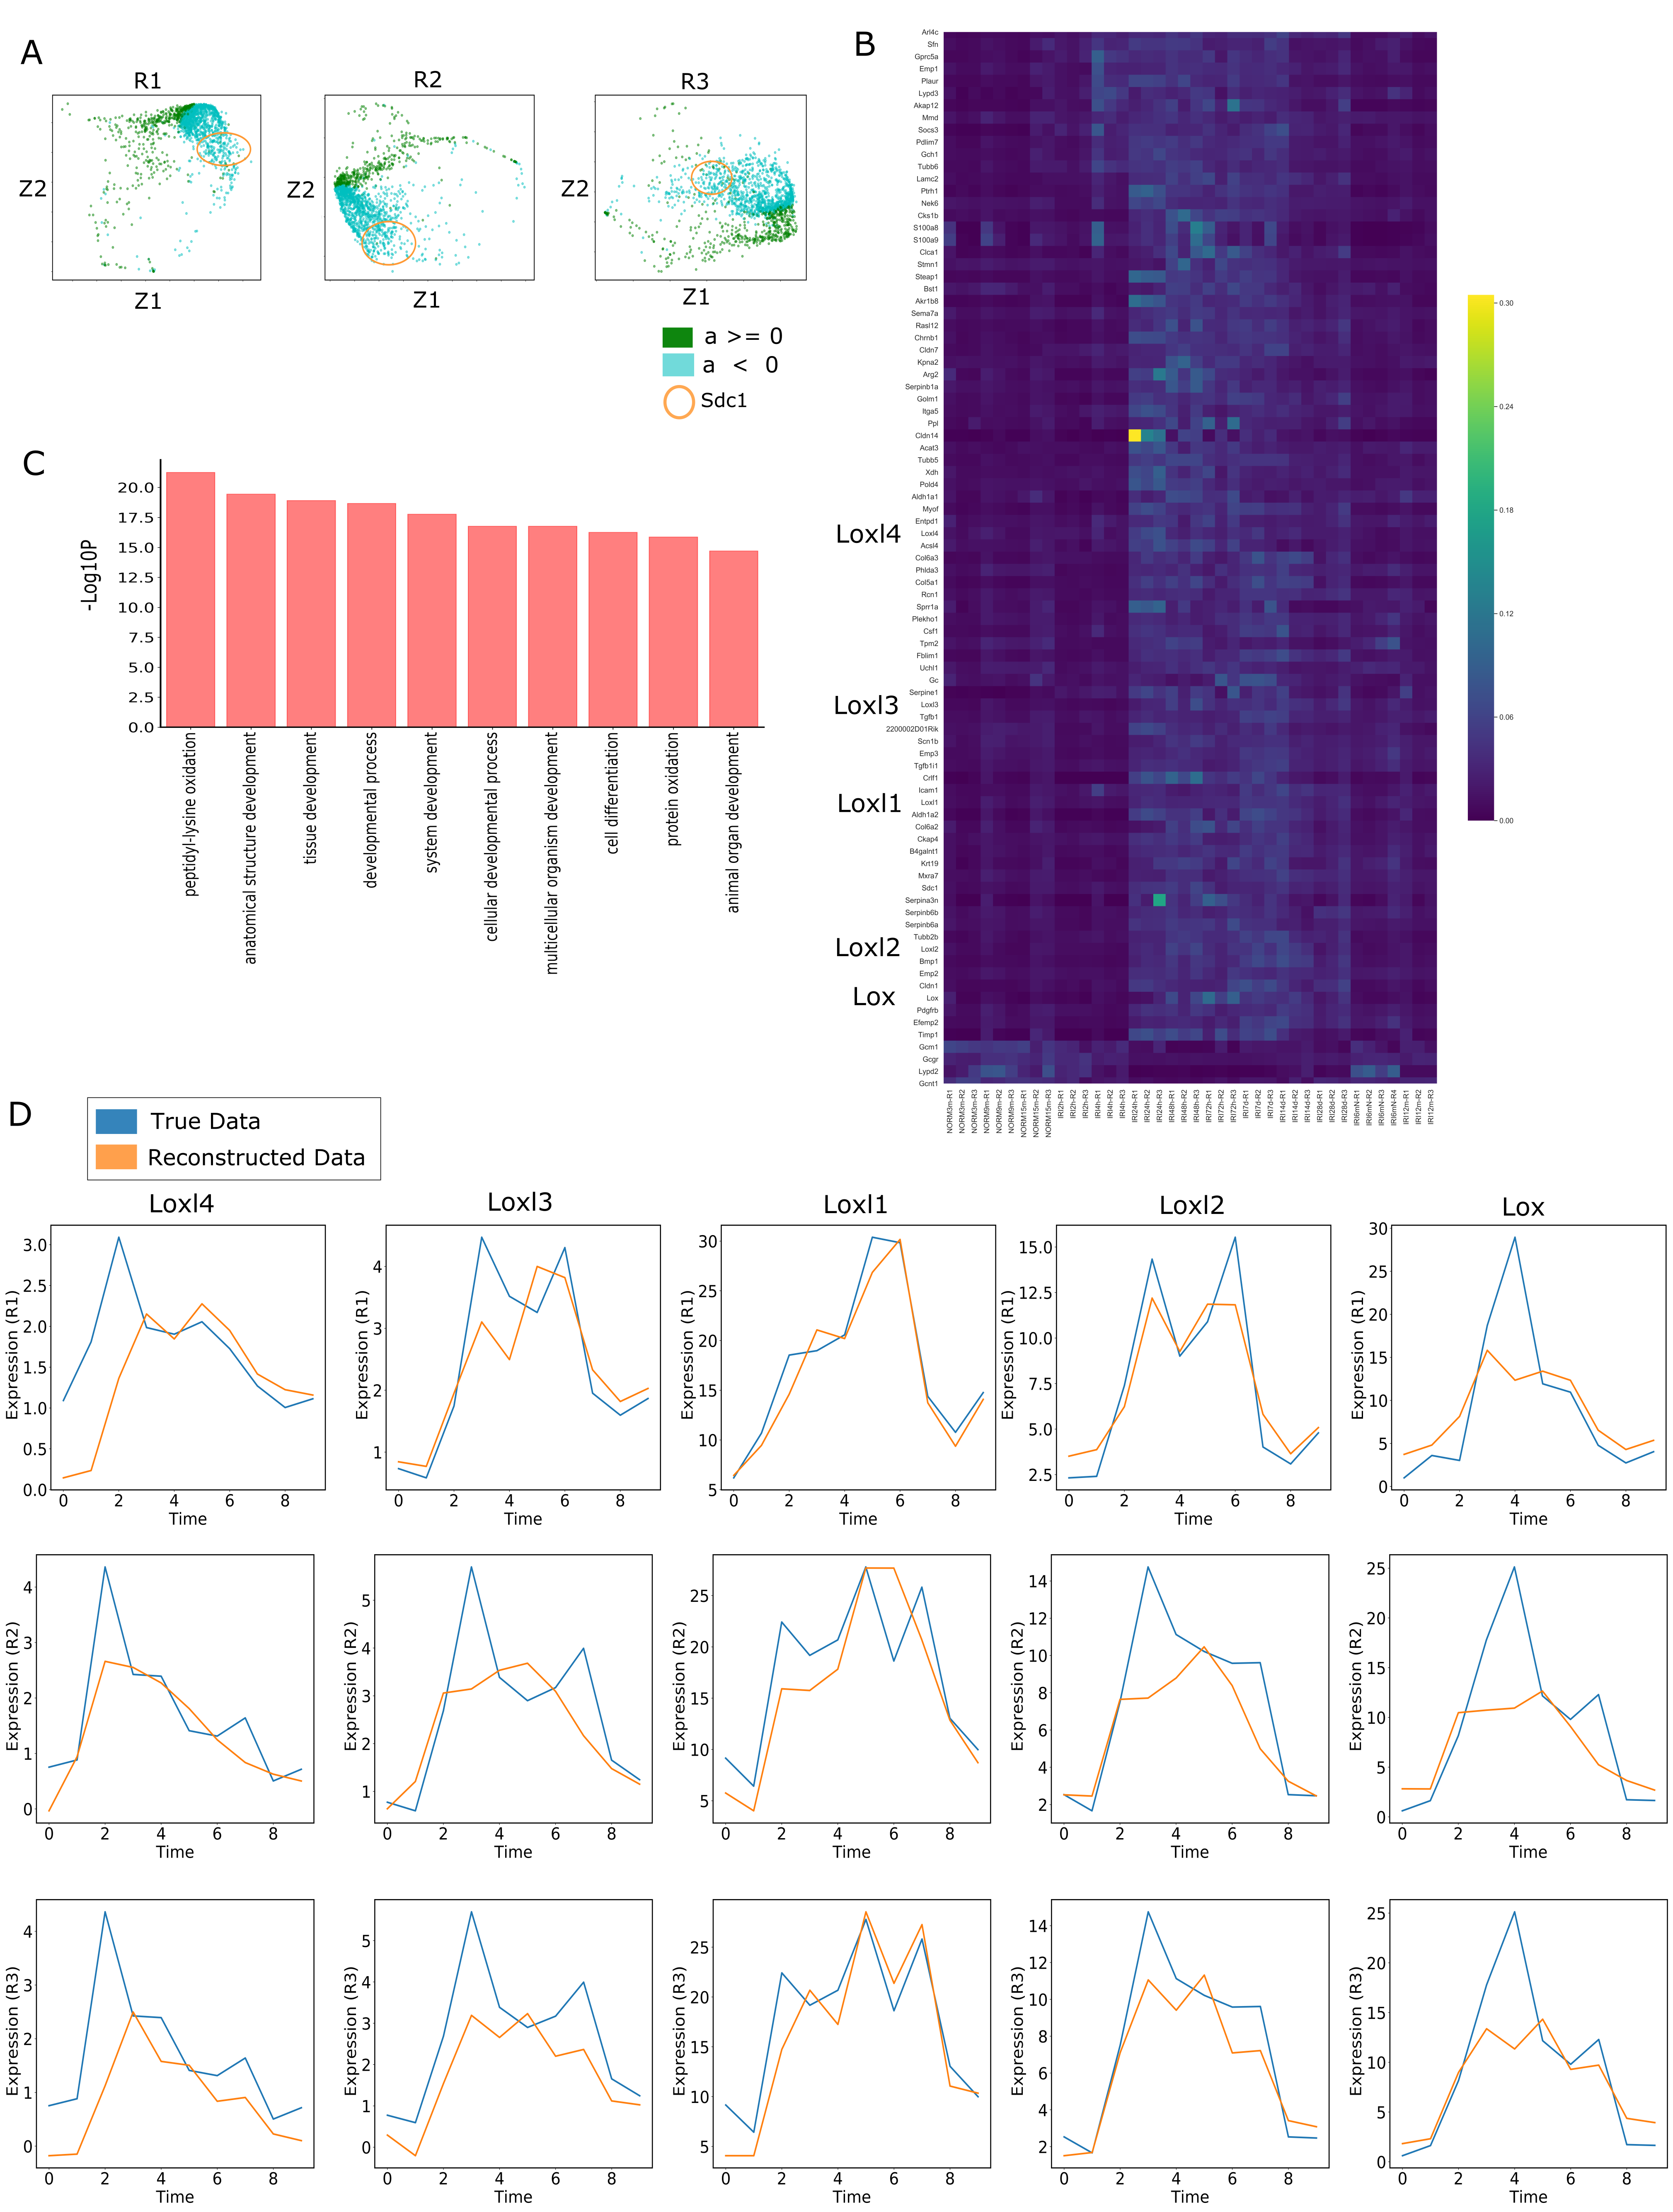
\includegraphics[width=\linewidth]{./figures/sdc_sl.png}
 % archetecture.png: 1149x508 px, 72dpi, 40.53x17.92 cm, bb=0 0 1149 508
    \caption[RVAgene latent space captures biological processes driving concordant gene expression changes (Sdc1).]{{\bf (A)} Latent space representations for replicates R1-R3 with local neighborhoods of Sdc1 marked (circles). ({\bf B}) Heatmap of expression changes over time course of injury for the Sdc1 neighborhood genes in the intersection of R1-R3; selected genes highlighted.  ({\bf C}) Histogram of -log10 p values of top GO terms for biological processes for gene set in (B).
    {\bf D}) Reconstructed vs true data plotted for each of the Lox genes identified in (B).}
  \label{fig:figS7}
\end{figure}
\end{center}

\begin{center}
\begin{figure}[H]
  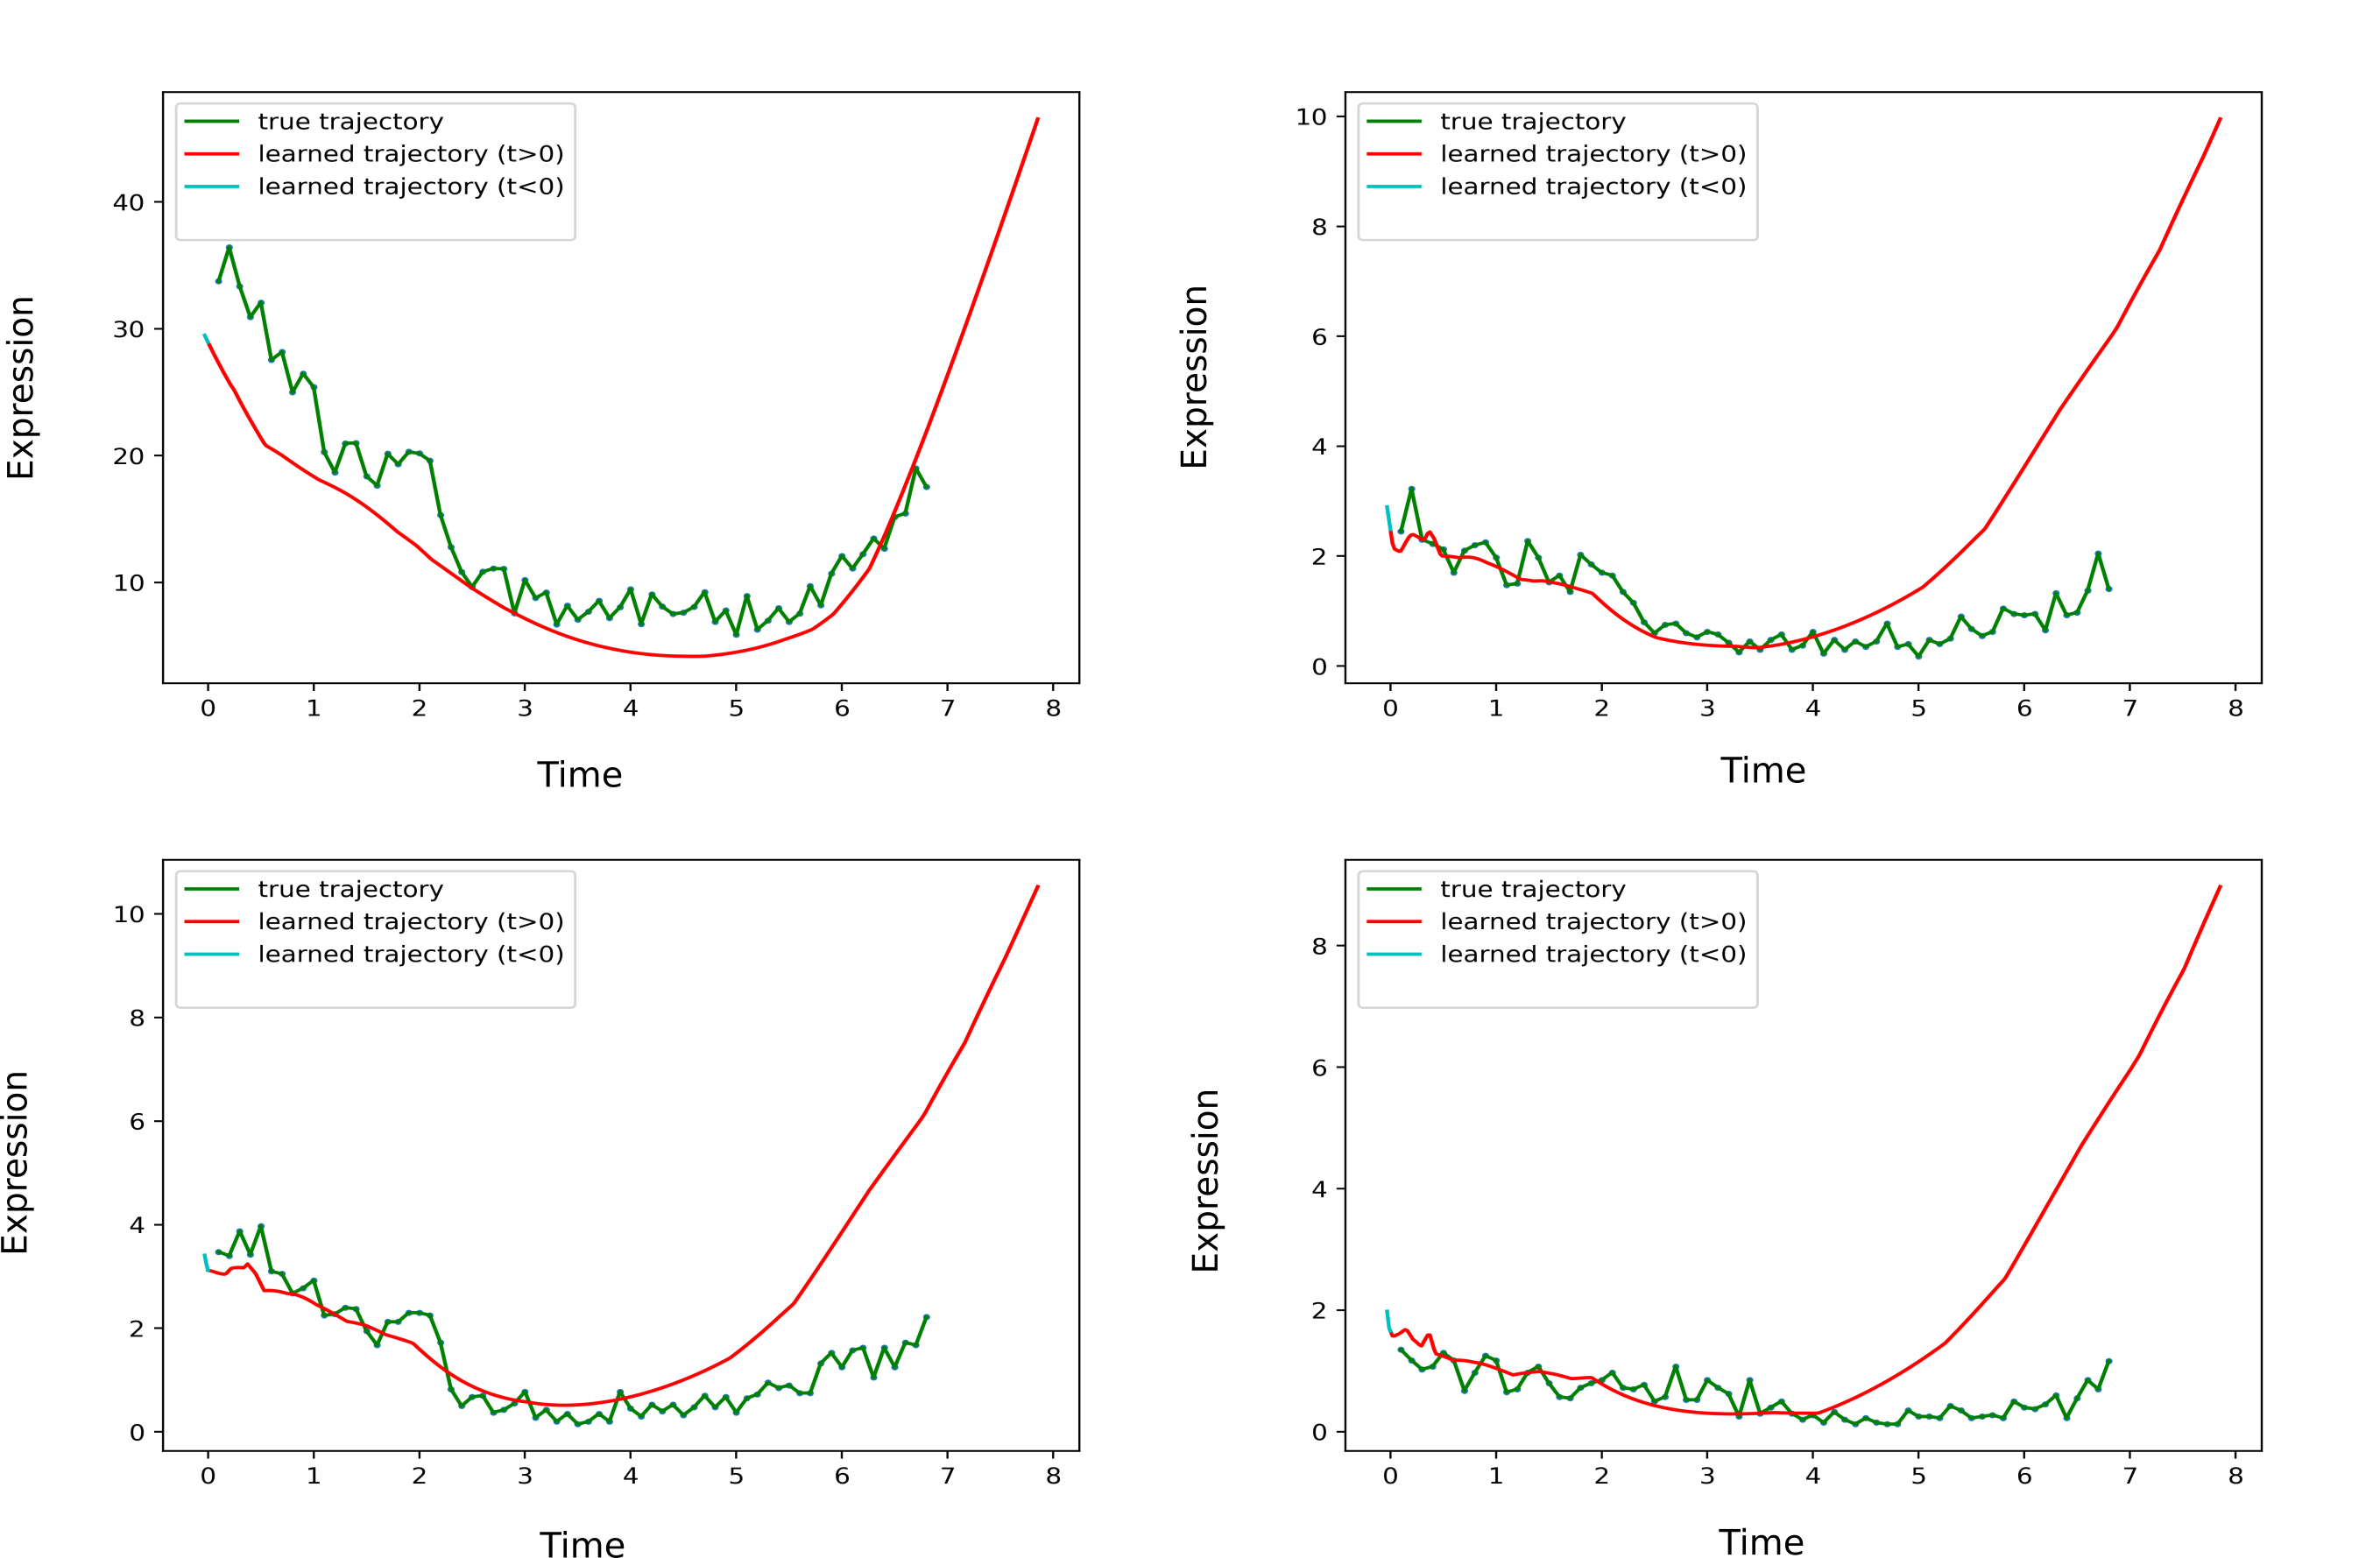
\includegraphics[width=\linewidth]{./figures/latent_ode_val_underfit.png}
 % archetecture.png: 1149x508 px, 72dpi, 40.53x17.92 cm, bb=0 0 1149 508
    \caption[Examples of continuous time prediction of ESC differentiation.]{\textbf{Examples of continuous time prediction of ESC differentiation.} Reconstruction (up to $t=6.8$) and future prediction (for $t>6.8$) for 4 example genes by a  latent ODE \citep{chen2018neural} trained on ESC data \citep{Klein2015} for 1000000 iterations, showing a good fit for the initial timepoints, but underfitting for the later timepoints.}
  \label{fig:figS9}
\end{figure}
\end{center}

%% RNASCAPE SUPP FIGURES
\begin{center}
\begin{figure}[H]
  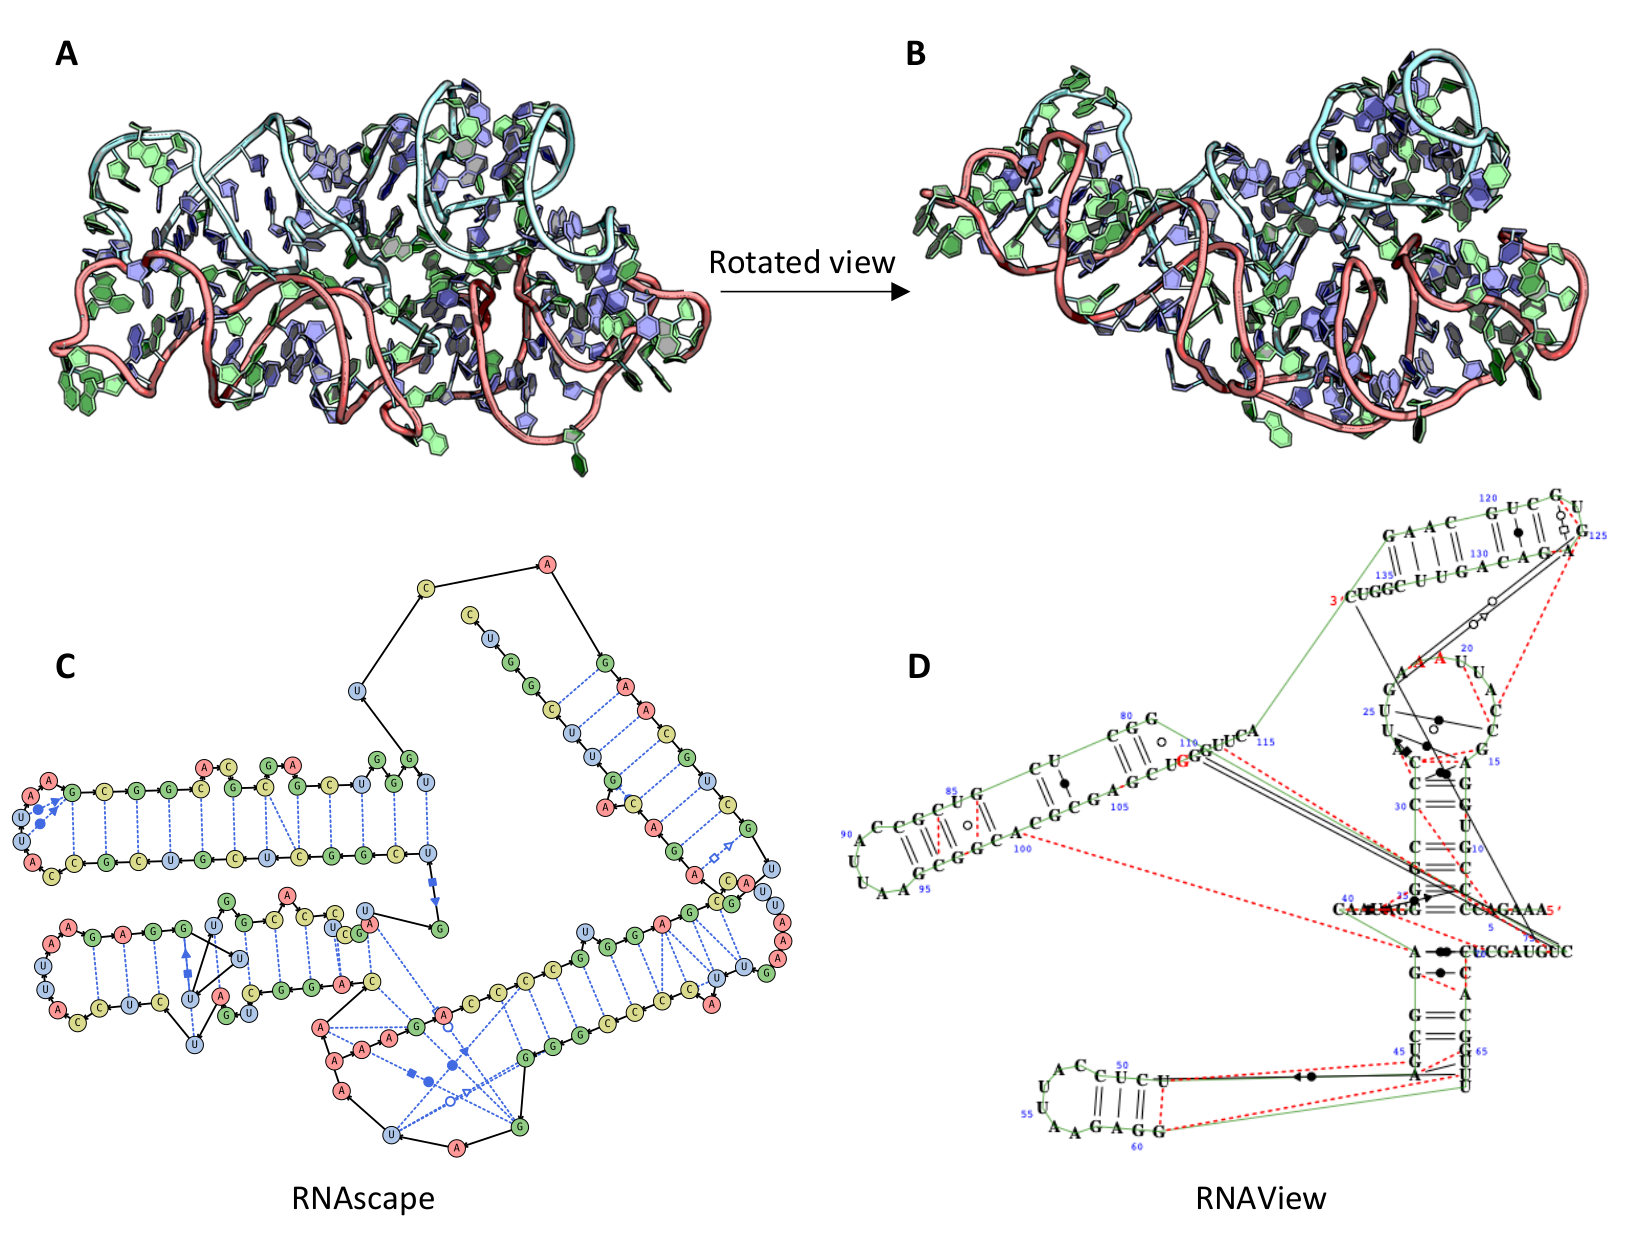
\includegraphics[width=\linewidth]{./rnascapefigs/figureS1.png}
 % archetecture.png: 1149x508 px, 72dpi, 40.53x17.92 cm, bb=0 0 1149 508
    \caption[Examples of continuous time prediction of ESC differentiation.]{\textbf{Examples of continuous time prediction of ESC differentiation.} Reconstruction (up to $t=6.8$) and future prediction (for $t>6.8$) for 4 example genes by a  latent ODE \citep{chen2018neural} trained on ESC data \citep{Klein2015} for 1000000 iterations, showing a good fit for the initial timepoints, but underfitting for the later timepoints.}
  \label{fig:rnascapeS1}
\end{figure}
\end{center}

\begin{center}
\begin{figure}[H]
  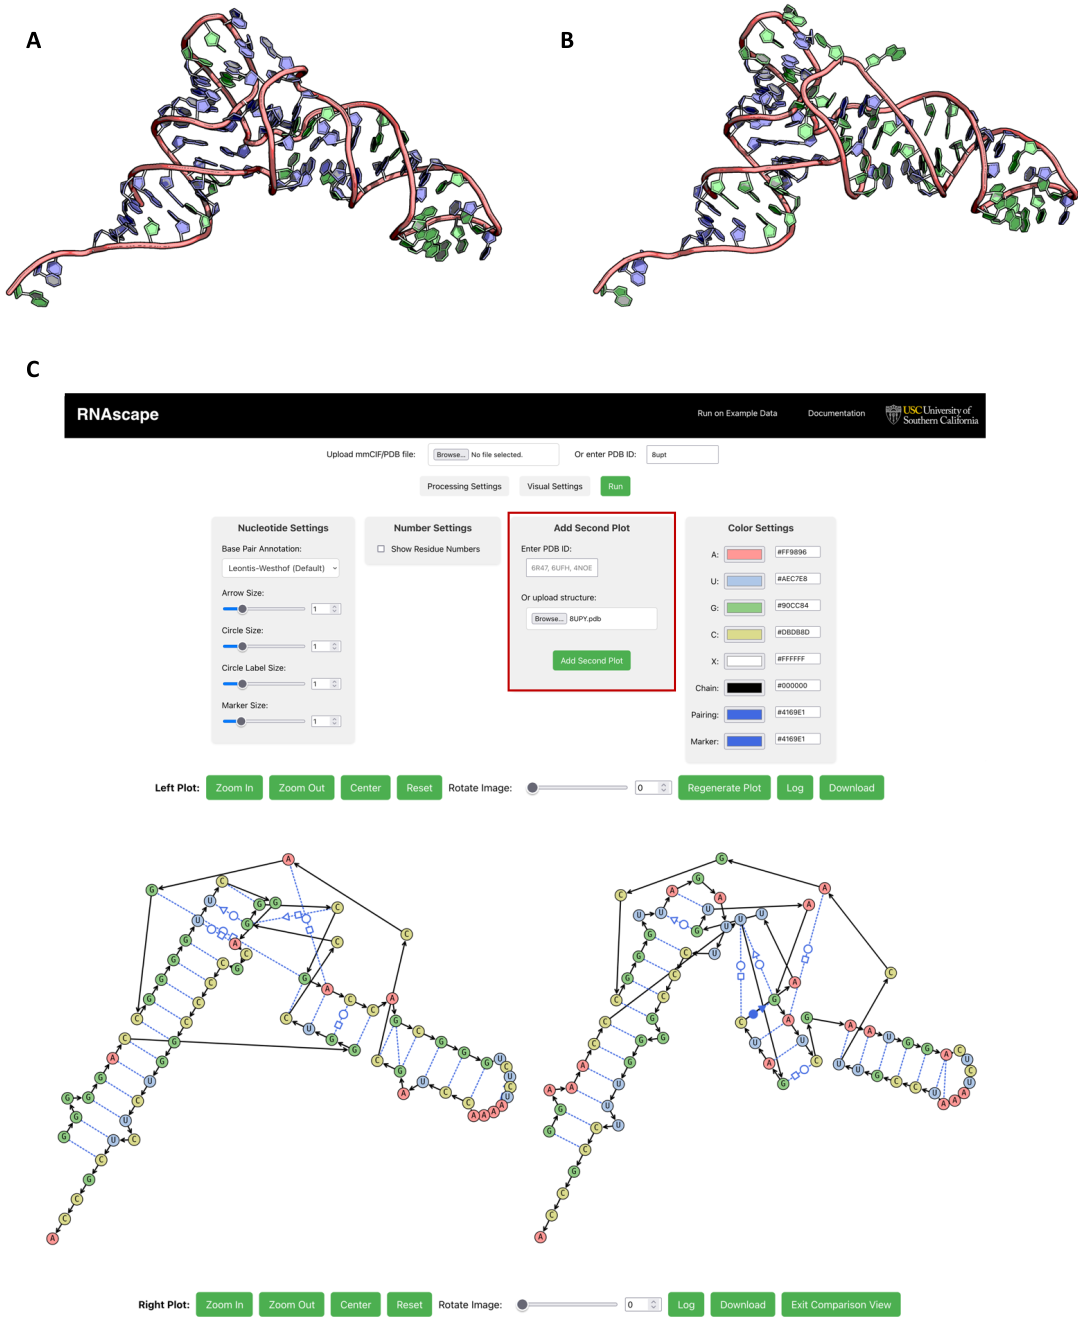
\includegraphics[width=\linewidth]{./rnascapefigs/figureS2.png}
 % archetecture.png: 1149x508 px, 72dpi, 40.53x17.92 cm, bb=0 0 1149 508
    \caption[Examples of continuous time prediction of ESC differentiation.]{\textbf{Examples of continuous time prediction of ESC differentiation.} Reconstruction (up to $t=6.8$) and future prediction (for $t>6.8$) for 4 example genes by a  latent ODE \citep{chen2018neural} trained on ESC data \citep{Klein2015} for 1000000 iterations, showing a good fit for the initial timepoints, but underfitting for the later timepoints.}
  \label{fig:rnascapeS2}
\end{figure}
\end{center}

\begin{center}
\begin{figure}[H]
  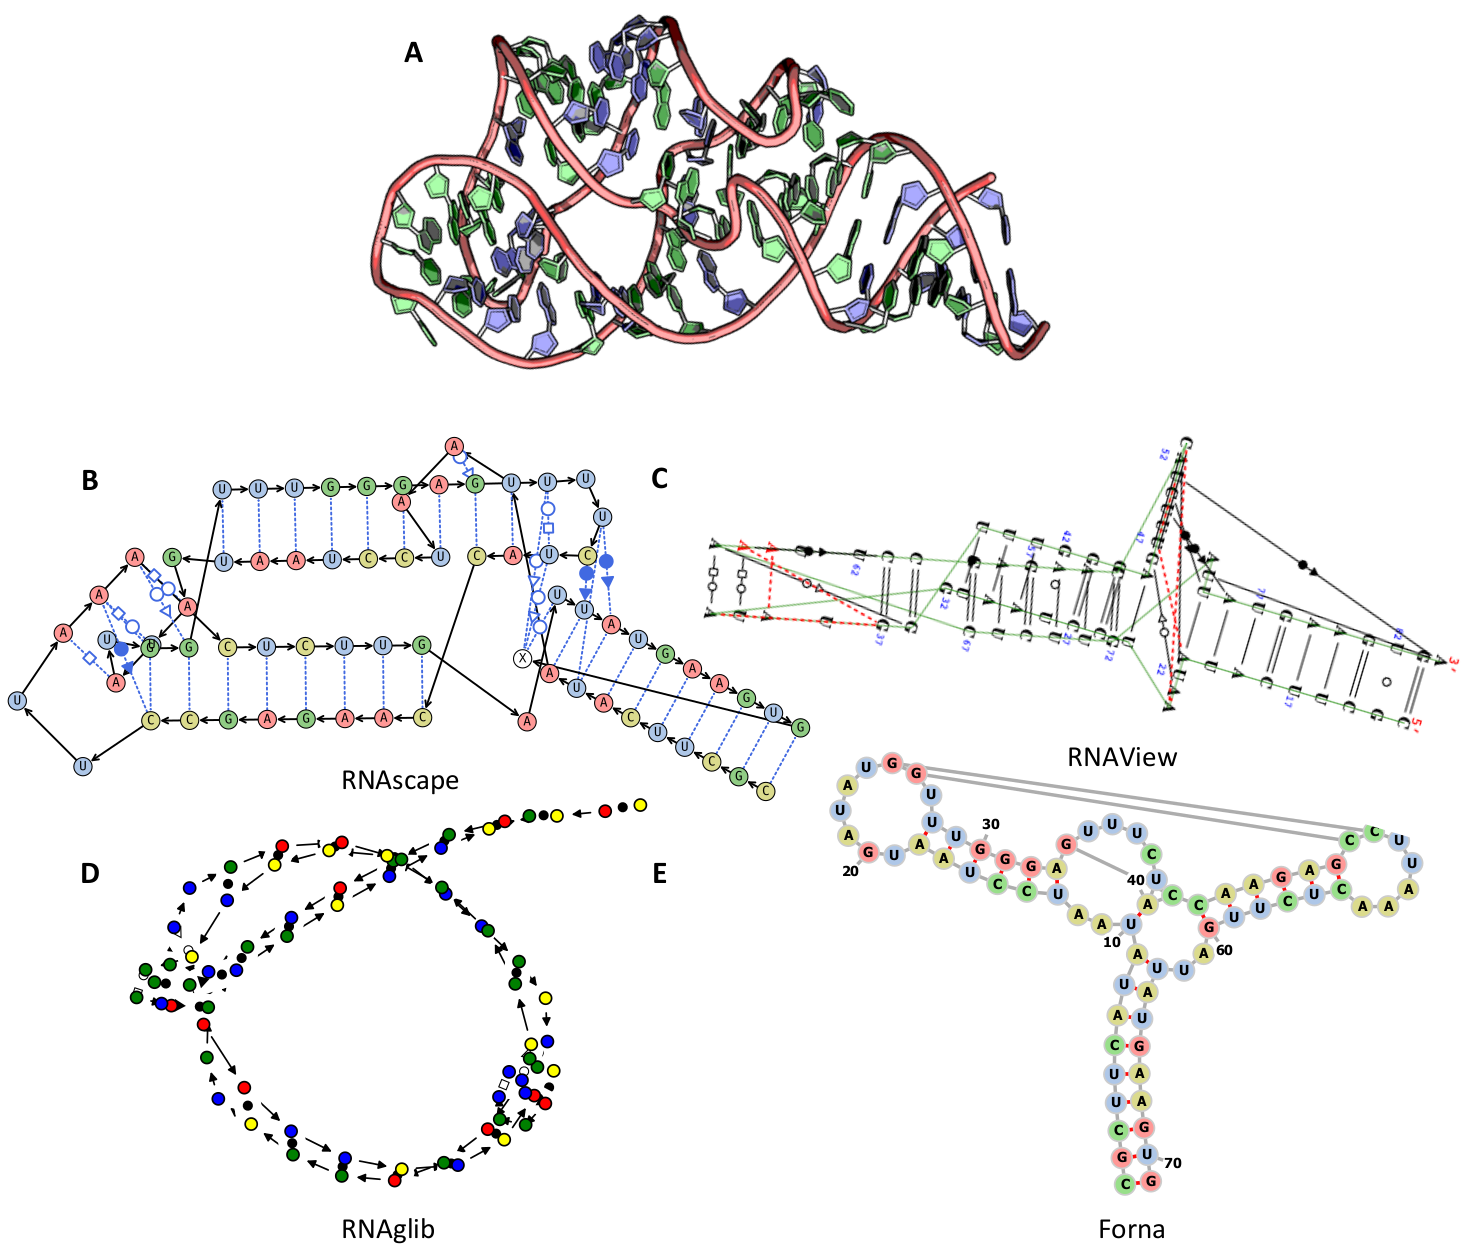
\includegraphics[width=\linewidth]{./rnascapefigs/figureS3.png}
 % archetecture.png: 1149x508 px, 72dpi, 40.53x17.92 cm, bb=0 0 1149 508
    \caption[Examples of continuous time prediction of ESC differentiation.]{\textbf{Examples of continuous time prediction of ESC differentiation.} Reconstruction (up to $t=6.8$) and future prediction (for $t>6.8$) for 4 example genes by a  latent ODE \citep{chen2018neural} trained on ESC data \citep{Klein2015} for 1000000 iterations, showing a good fit for the initial timepoints, but underfitting for the later timepoints.}
  \label{fig:rnascapeS3}
\end{figure}
\end{center}

%% DeepPBS SUPP FIGURES
\begin{center}
\begin{figure}[H]
  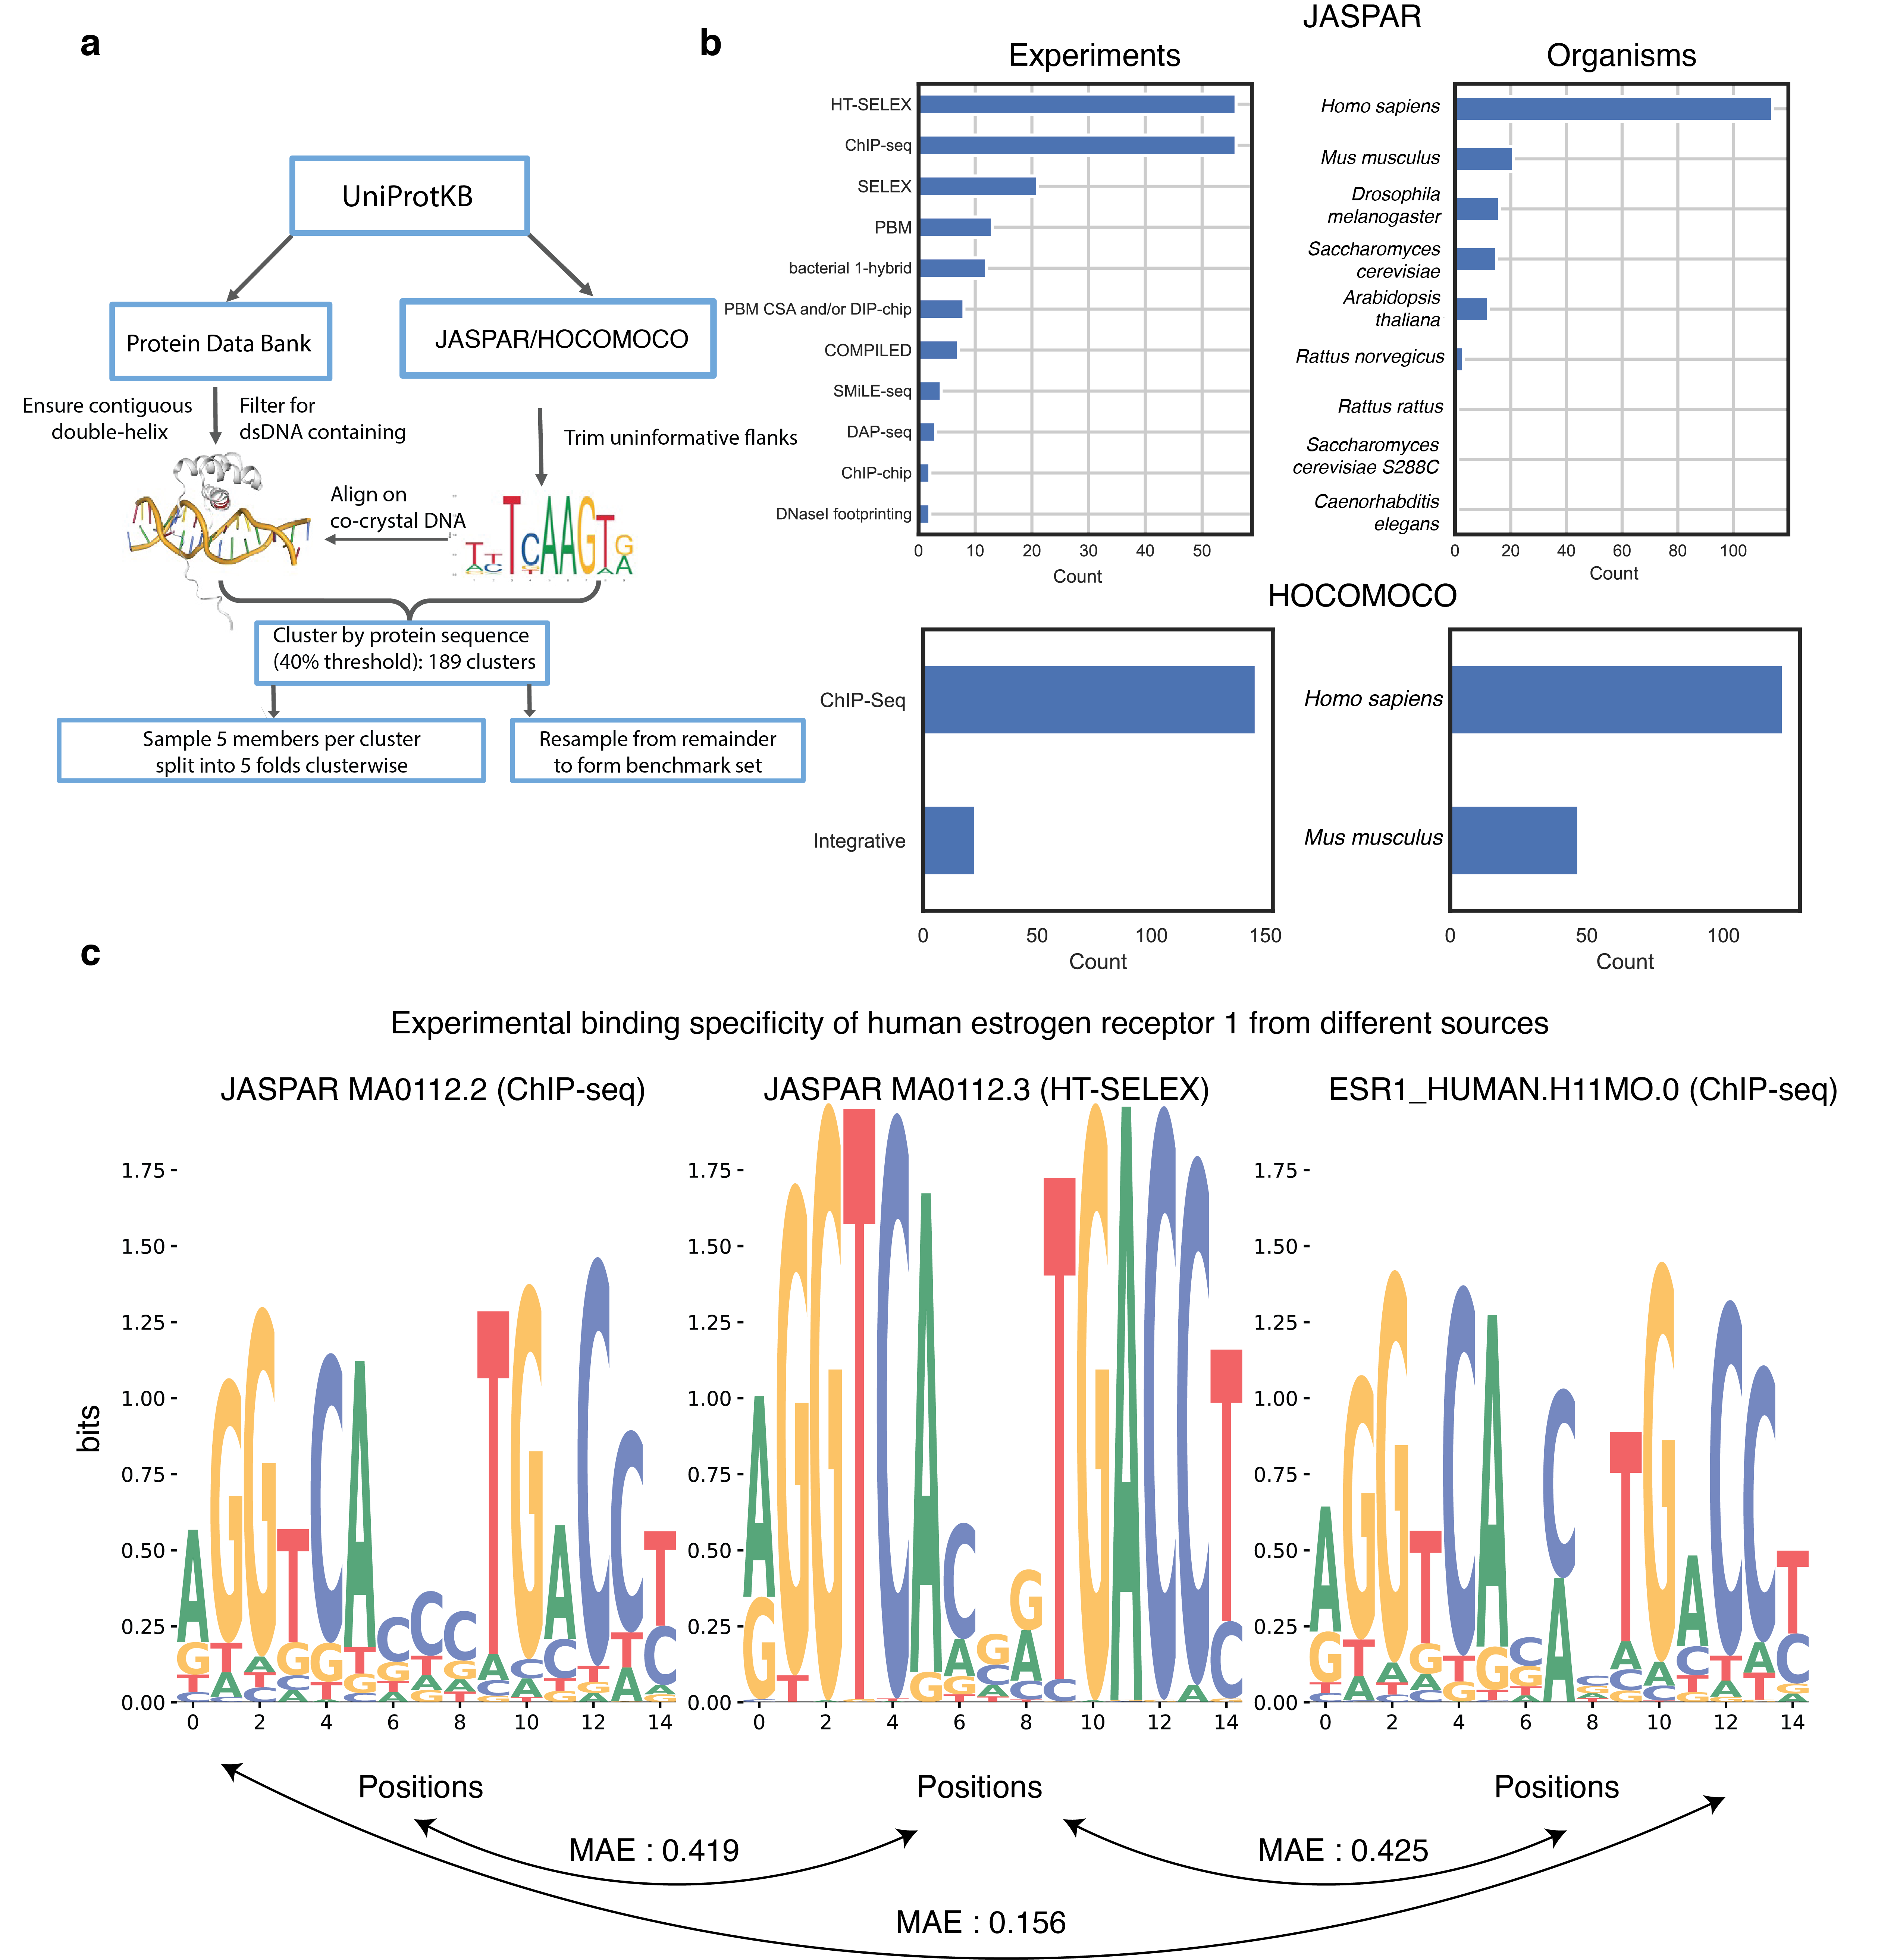
\includegraphics[width=\linewidth]{./pdnafigs/figS1.png}
 % archetecture.png: 1149x508 px, 72dpi, 40.53x17.92 cm, bb=0 0 1149 508
    \caption[Examples of continuous time prediction of ESC differentiation.]{\textbf{Examples of continuous time prediction of ESC differentiation.} Reconstruction (up to $t=6.8$) and future prediction (for $t>6.8$) for 4 example genes by a  latent ODE \citep{chen2018neural} trained on ESC data \citep{Klein2015} for 1000000 iterations, showing a good fit for the initial timepoints, but underfitting for the later timepoints.}
  \label{fig:pdnaS1}
\end{figure}
\end{center}

\begin{center}
\begin{figure}[H]
  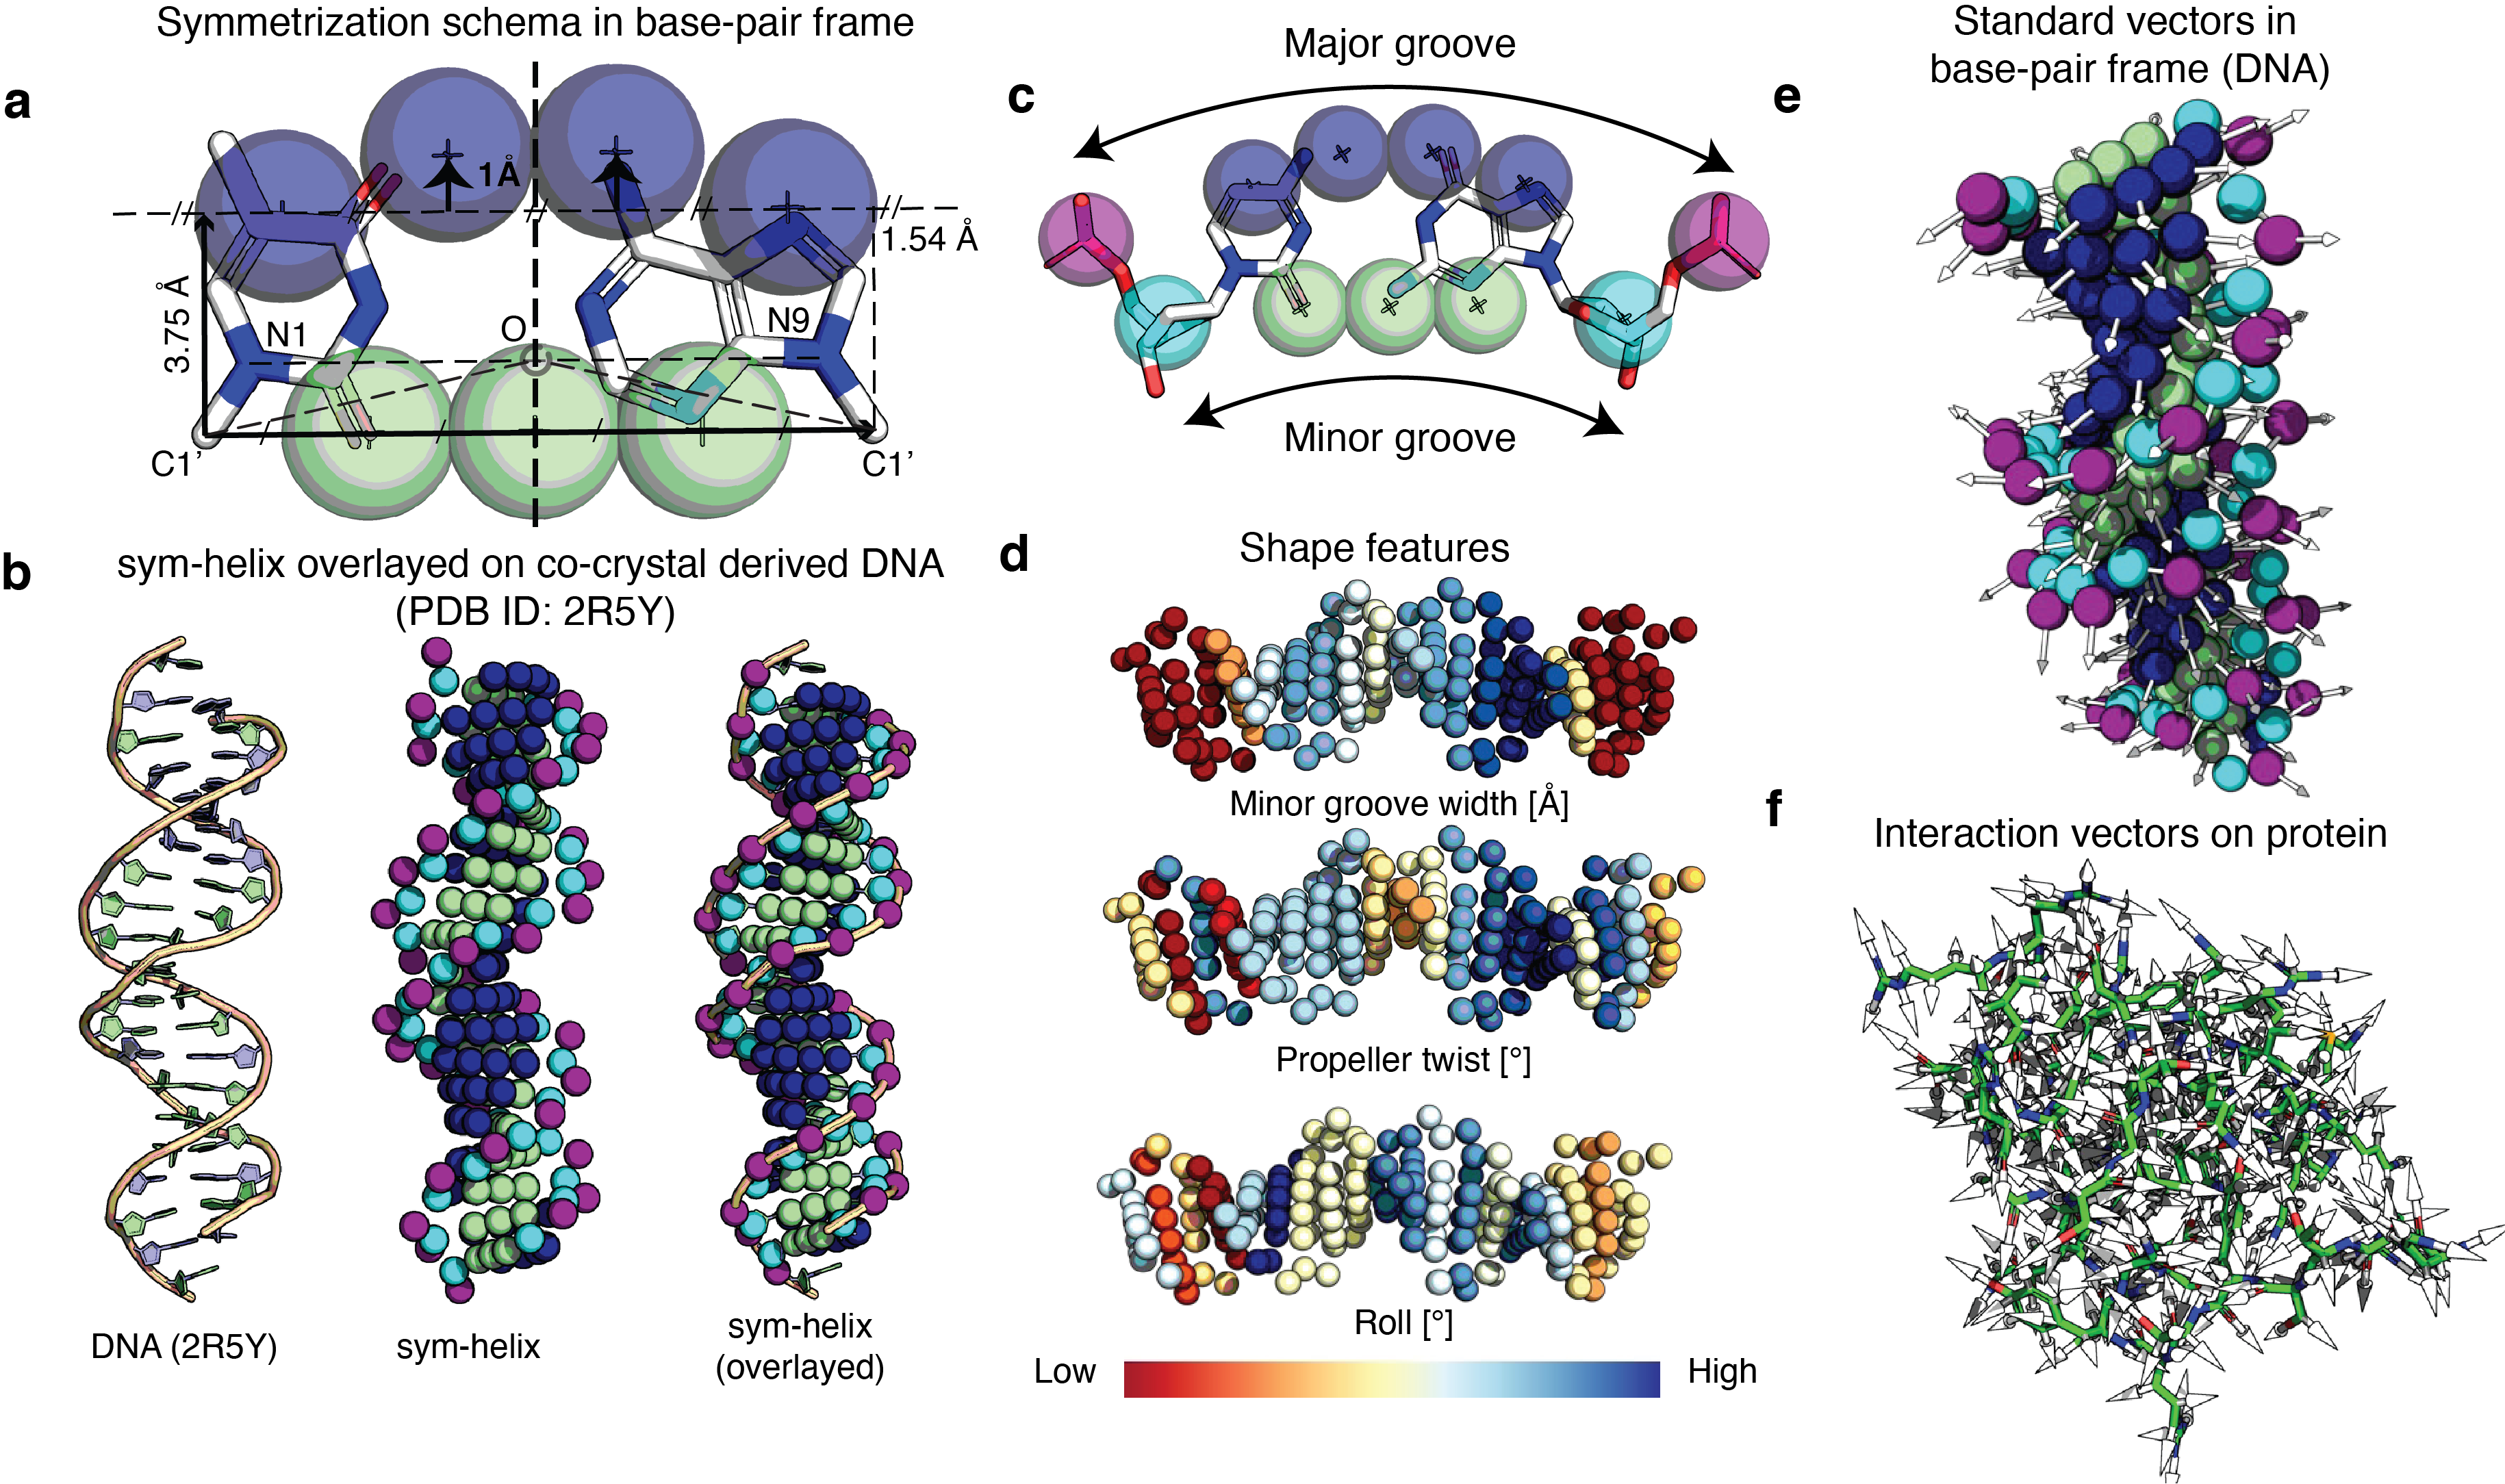
\includegraphics[width=\linewidth]{./pdnafigs/figS2.png}
 % archetecture.png: 1149x508 px, 72dpi, 40.53x17.92 cm, bb=0 0 1149 508
    \caption[Examples of continuous time prediction of ESC differentiation.]{\textbf{Examples of continuous time prediction of ESC differentiation.} Reconstruction (up to $t=6.8$) and future prediction (for $t>6.8$) for 4 example genes by a  latent ODE \citep{chen2018neural} trained on ESC data \citep{Klein2015} for 1000000 iterations, showing a good fit for the initial timepoints, but underfitting for the later timepoints.}
  \label{fig:pdnaS2}
\end{figure}
\end{center}

\begin{center}
\begin{figure}[H]
  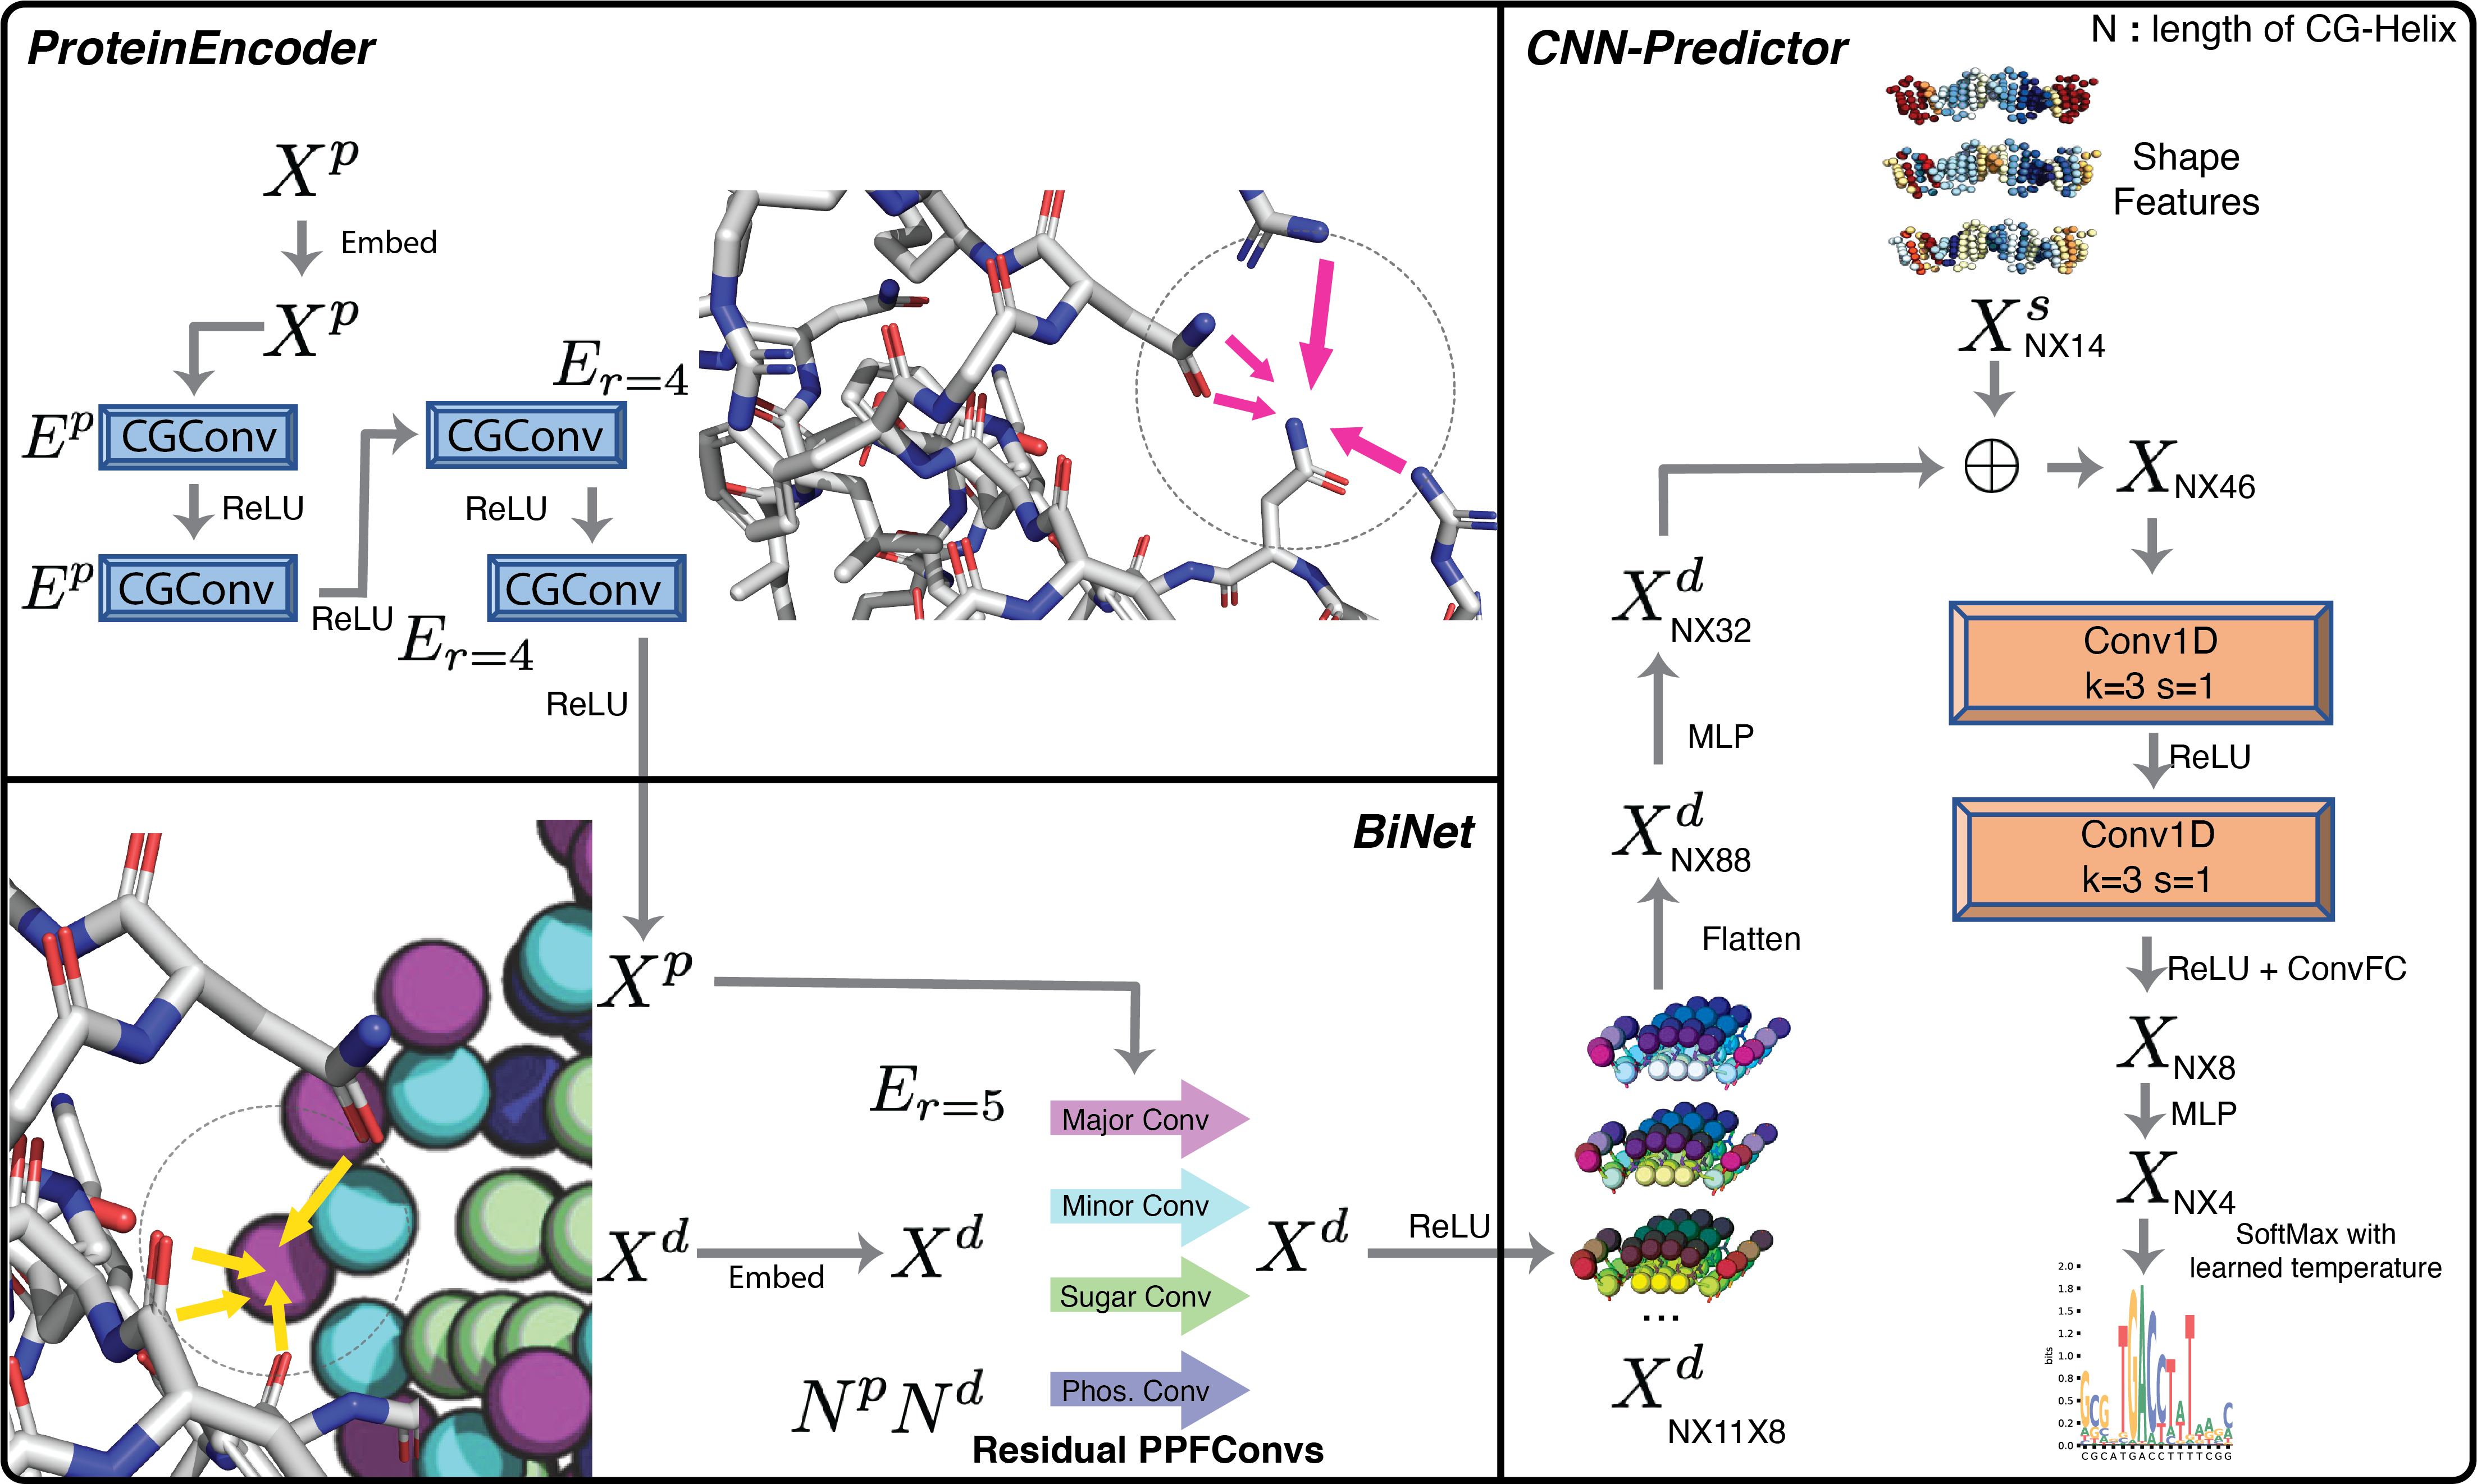
\includegraphics[width=\linewidth]{./pdnafigs/figS3.png}
 % archetecture.png: 1149x508 px, 72dpi, 40.53x17.92 cm, bb=0 0 1149 508
    \caption[Examples of continuous time prediction of ESC differentiation.]{\textbf{Examples of continuous time prediction of ESC differentiation.} Reconstruction (up to $t=6.8$) and future prediction (for $t>6.8$) for 4 example genes by a  latent ODE \citep{chen2018neural} trained on ESC data \citep{Klein2015} for 1000000 iterations, showing a good fit for the initial timepoints, but underfitting for the later timepoints.}
  \label{fig:pdnaS3}
\end{figure}
\end{center}

\begin{center}
\begin{figure}[H]
  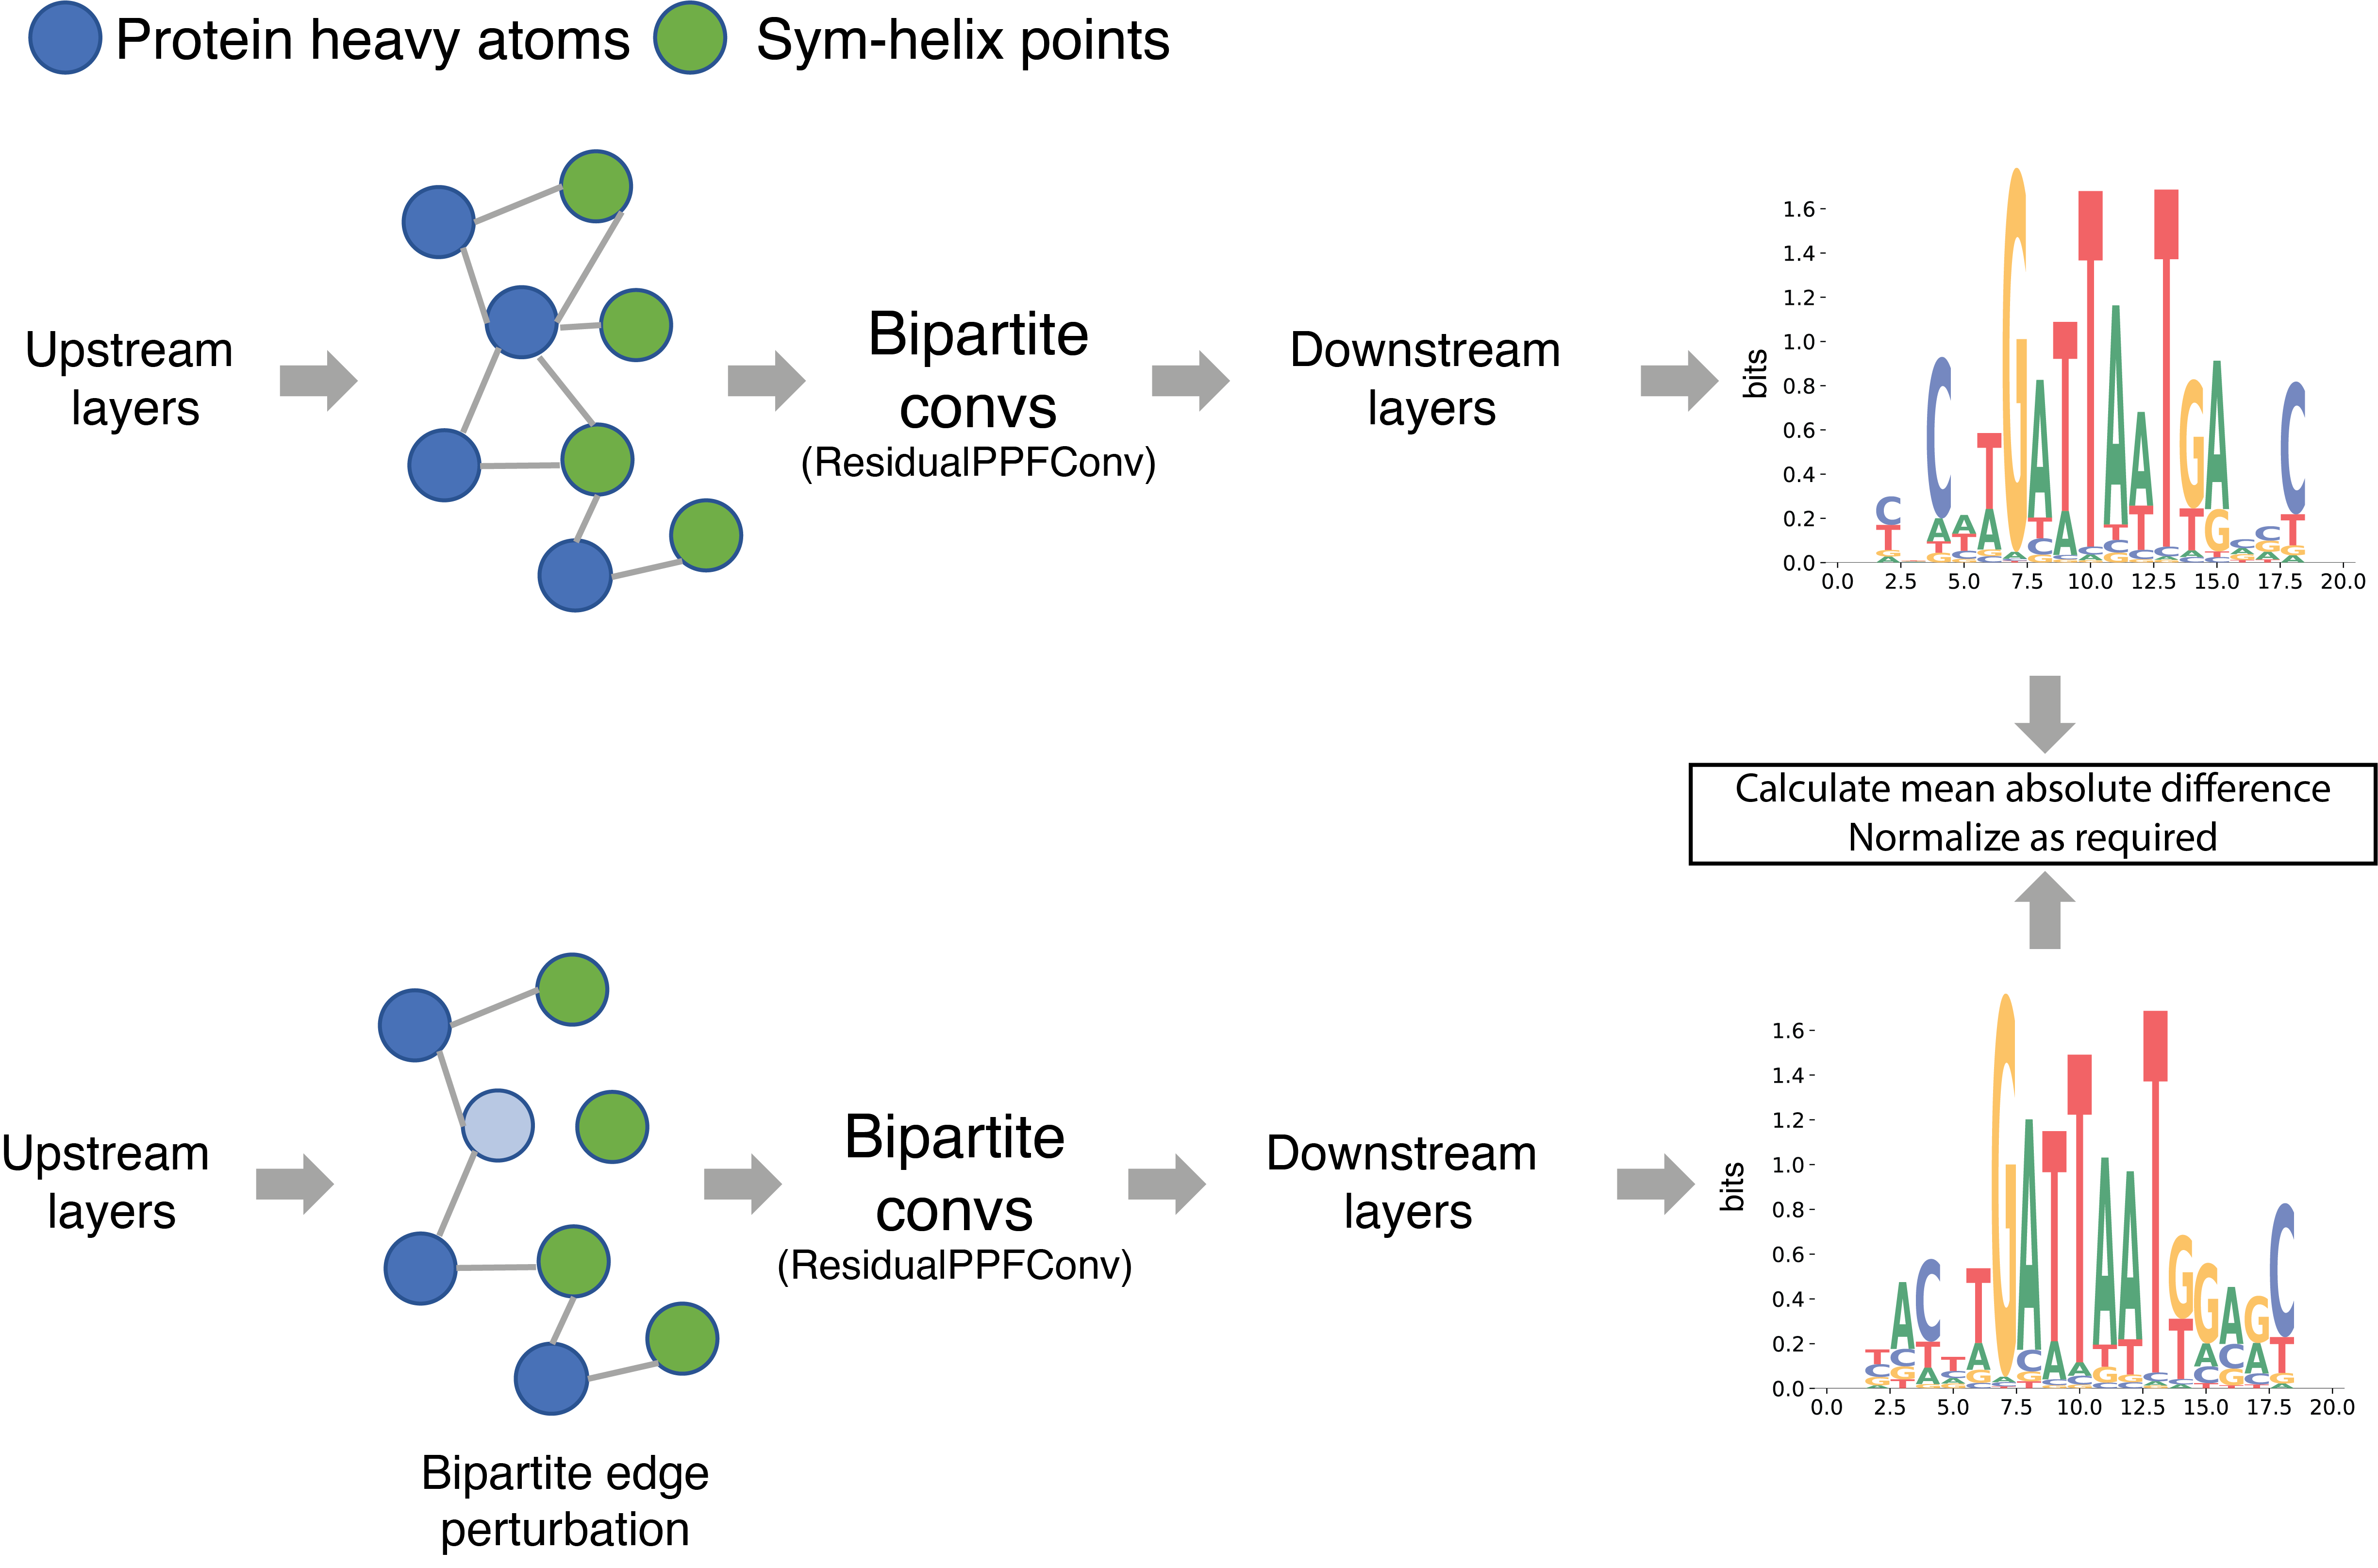
\includegraphics[width=\linewidth]{./pdnafigs/figS4.png}
 % archetecture.png: 1149x508 px, 72dpi, 40.53x17.92 cm, bb=0 0 1149 508
    \caption[Examples of continuous time prediction of ESC differentiation.]{\textbf{Examples of continuous time prediction of ESC differentiation.} Reconstruction (up to $t=6.8$) and future prediction (for $t>6.8$) for 4 example genes by a  latent ODE \citep{chen2018neural} trained on ESC data \citep{Klein2015} for 1000000 iterations, showing a good fit for the initial timepoints, but underfitting for the later timepoints.}
  \label{fig:pdnaS4}
\end{figure}
\end{center}

\begin{center}
\begin{figure}[H]
  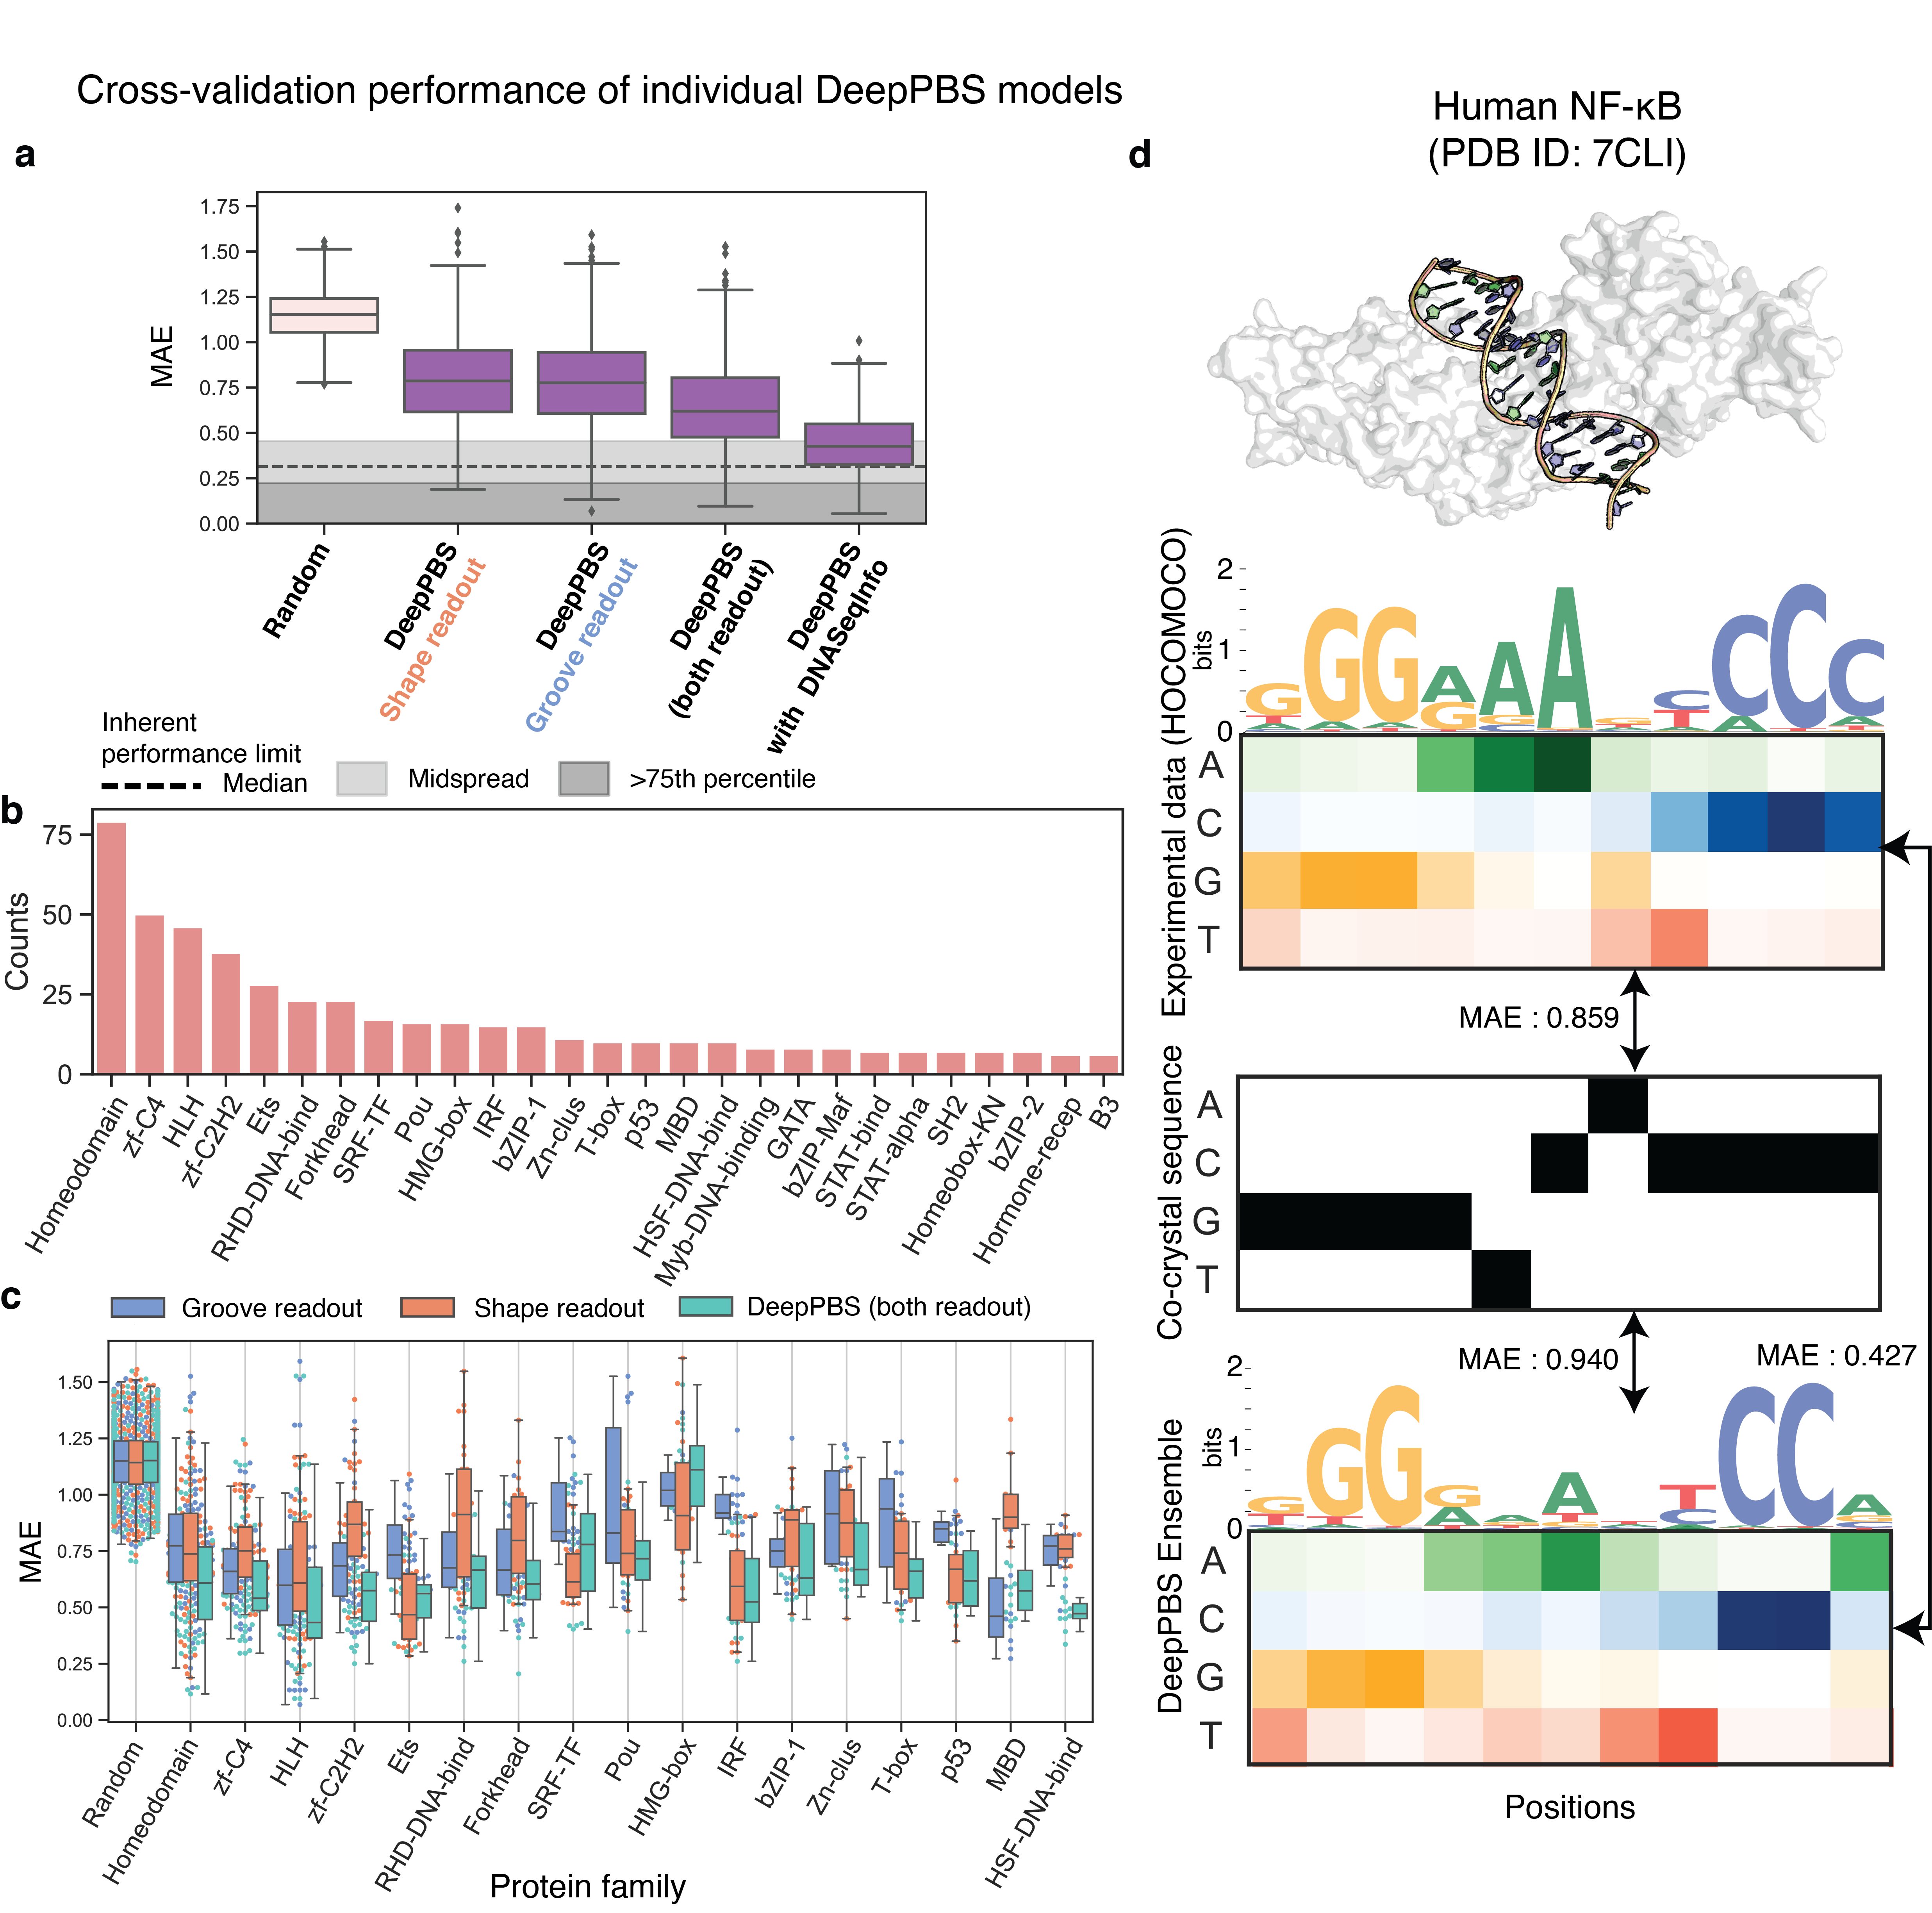
\includegraphics[width=\linewidth]{./pdnafigs/figS5.png}
 % archetecture.png: 1149x508 px, 72dpi, 40.53x17.92 cm, bb=0 0 1149 508
    \caption[Examples of continuous time prediction of ESC differentiation.]{\textbf{Examples of continuous time prediction of ESC differentiation.} Reconstruction (up to $t=6.8$) and future prediction (for $t>6.8$) for 4 example genes by a  latent ODE \citep{chen2018neural} trained on ESC data \citep{Klein2015} for 1000000 iterations, showing a good fit for the initial timepoints, but underfitting for the later timepoints.}
  \label{fig:pdnaS5}
\end{figure}
\end{center}

\begin{center}
\begin{figure}[H]
  \includegraphics[width=\linewidth]{./pdnafigs/figS6.png}
 % archetecture.png: 1149x508 px, 72dpi, 40.53x17.92 cm, bb=0 0 1149 508
    \caption[Examples of continuous time prediction of ESC differentiation.]{\textbf{Examples of continuous time prediction of ESC differentiation.} Reconstruction (up to $t=6.8$) and future prediction (for $t>6.8$) for 4 example genes by a  latent ODE \citep{chen2018neural} trained on ESC data \citep{Klein2015} for 1000000 iterations, showing a good fit for the initial timepoints, but underfitting for the later timepoints.}
  \label{fig:pdnaS6}
\end{figure}
\end{center}

\begin{center}
\begin{figure}[H]
  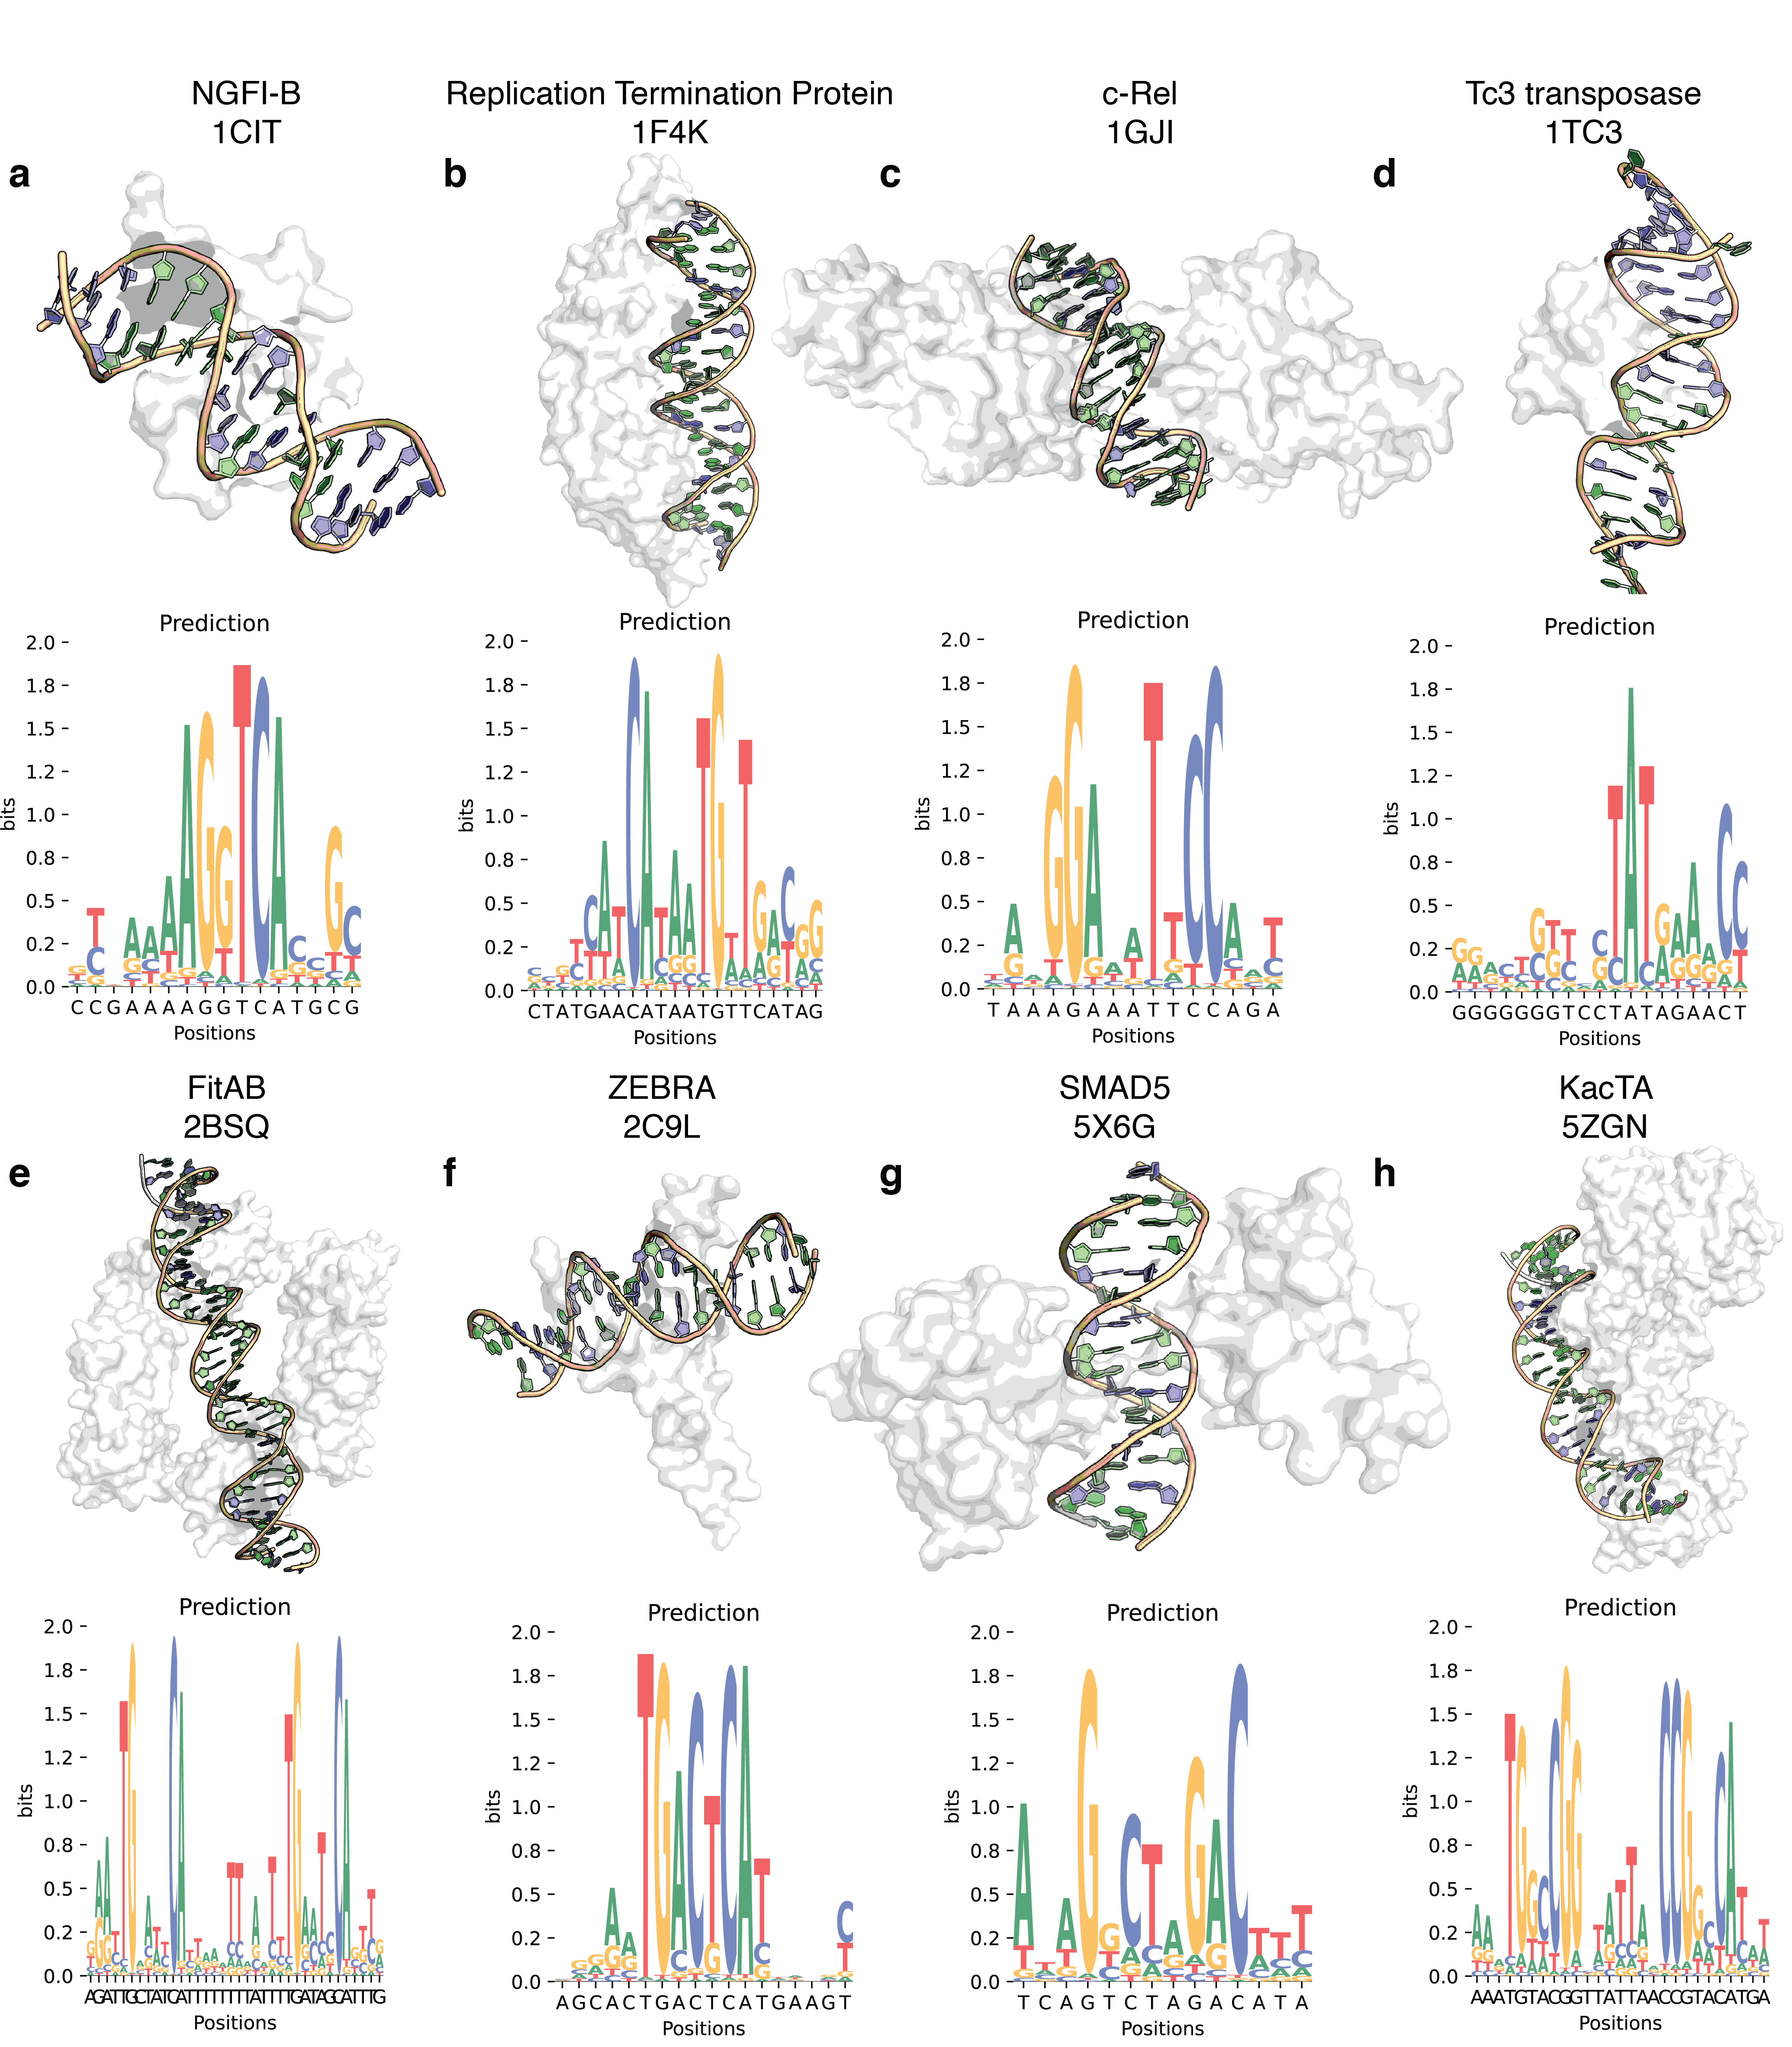
\includegraphics[width=\linewidth]{./pdnafigs/figS7.png}
 % archetecture.png: 1149x508 px, 72dpi, 40.53x17.92 cm, bb=0 0 1149 508
    \caption[Examples of continuous time prediction of ESC differentiation.]{\textbf{Examples of continuous time prediction of ESC differentiation.} Reconstruction (up to $t=6.8$) and future prediction (for $t>6.8$) for 4 example genes by a  latent ODE \citep{chen2018neural} trained on ESC data \citep{Klein2015} for 1000000 iterations, showing a good fit for the initial timepoints, but underfitting for the later timepoints.}
  \label{fig:pdnaS7}
\end{figure}
\end{center}

\begin{center}
\begin{figure}[H]
  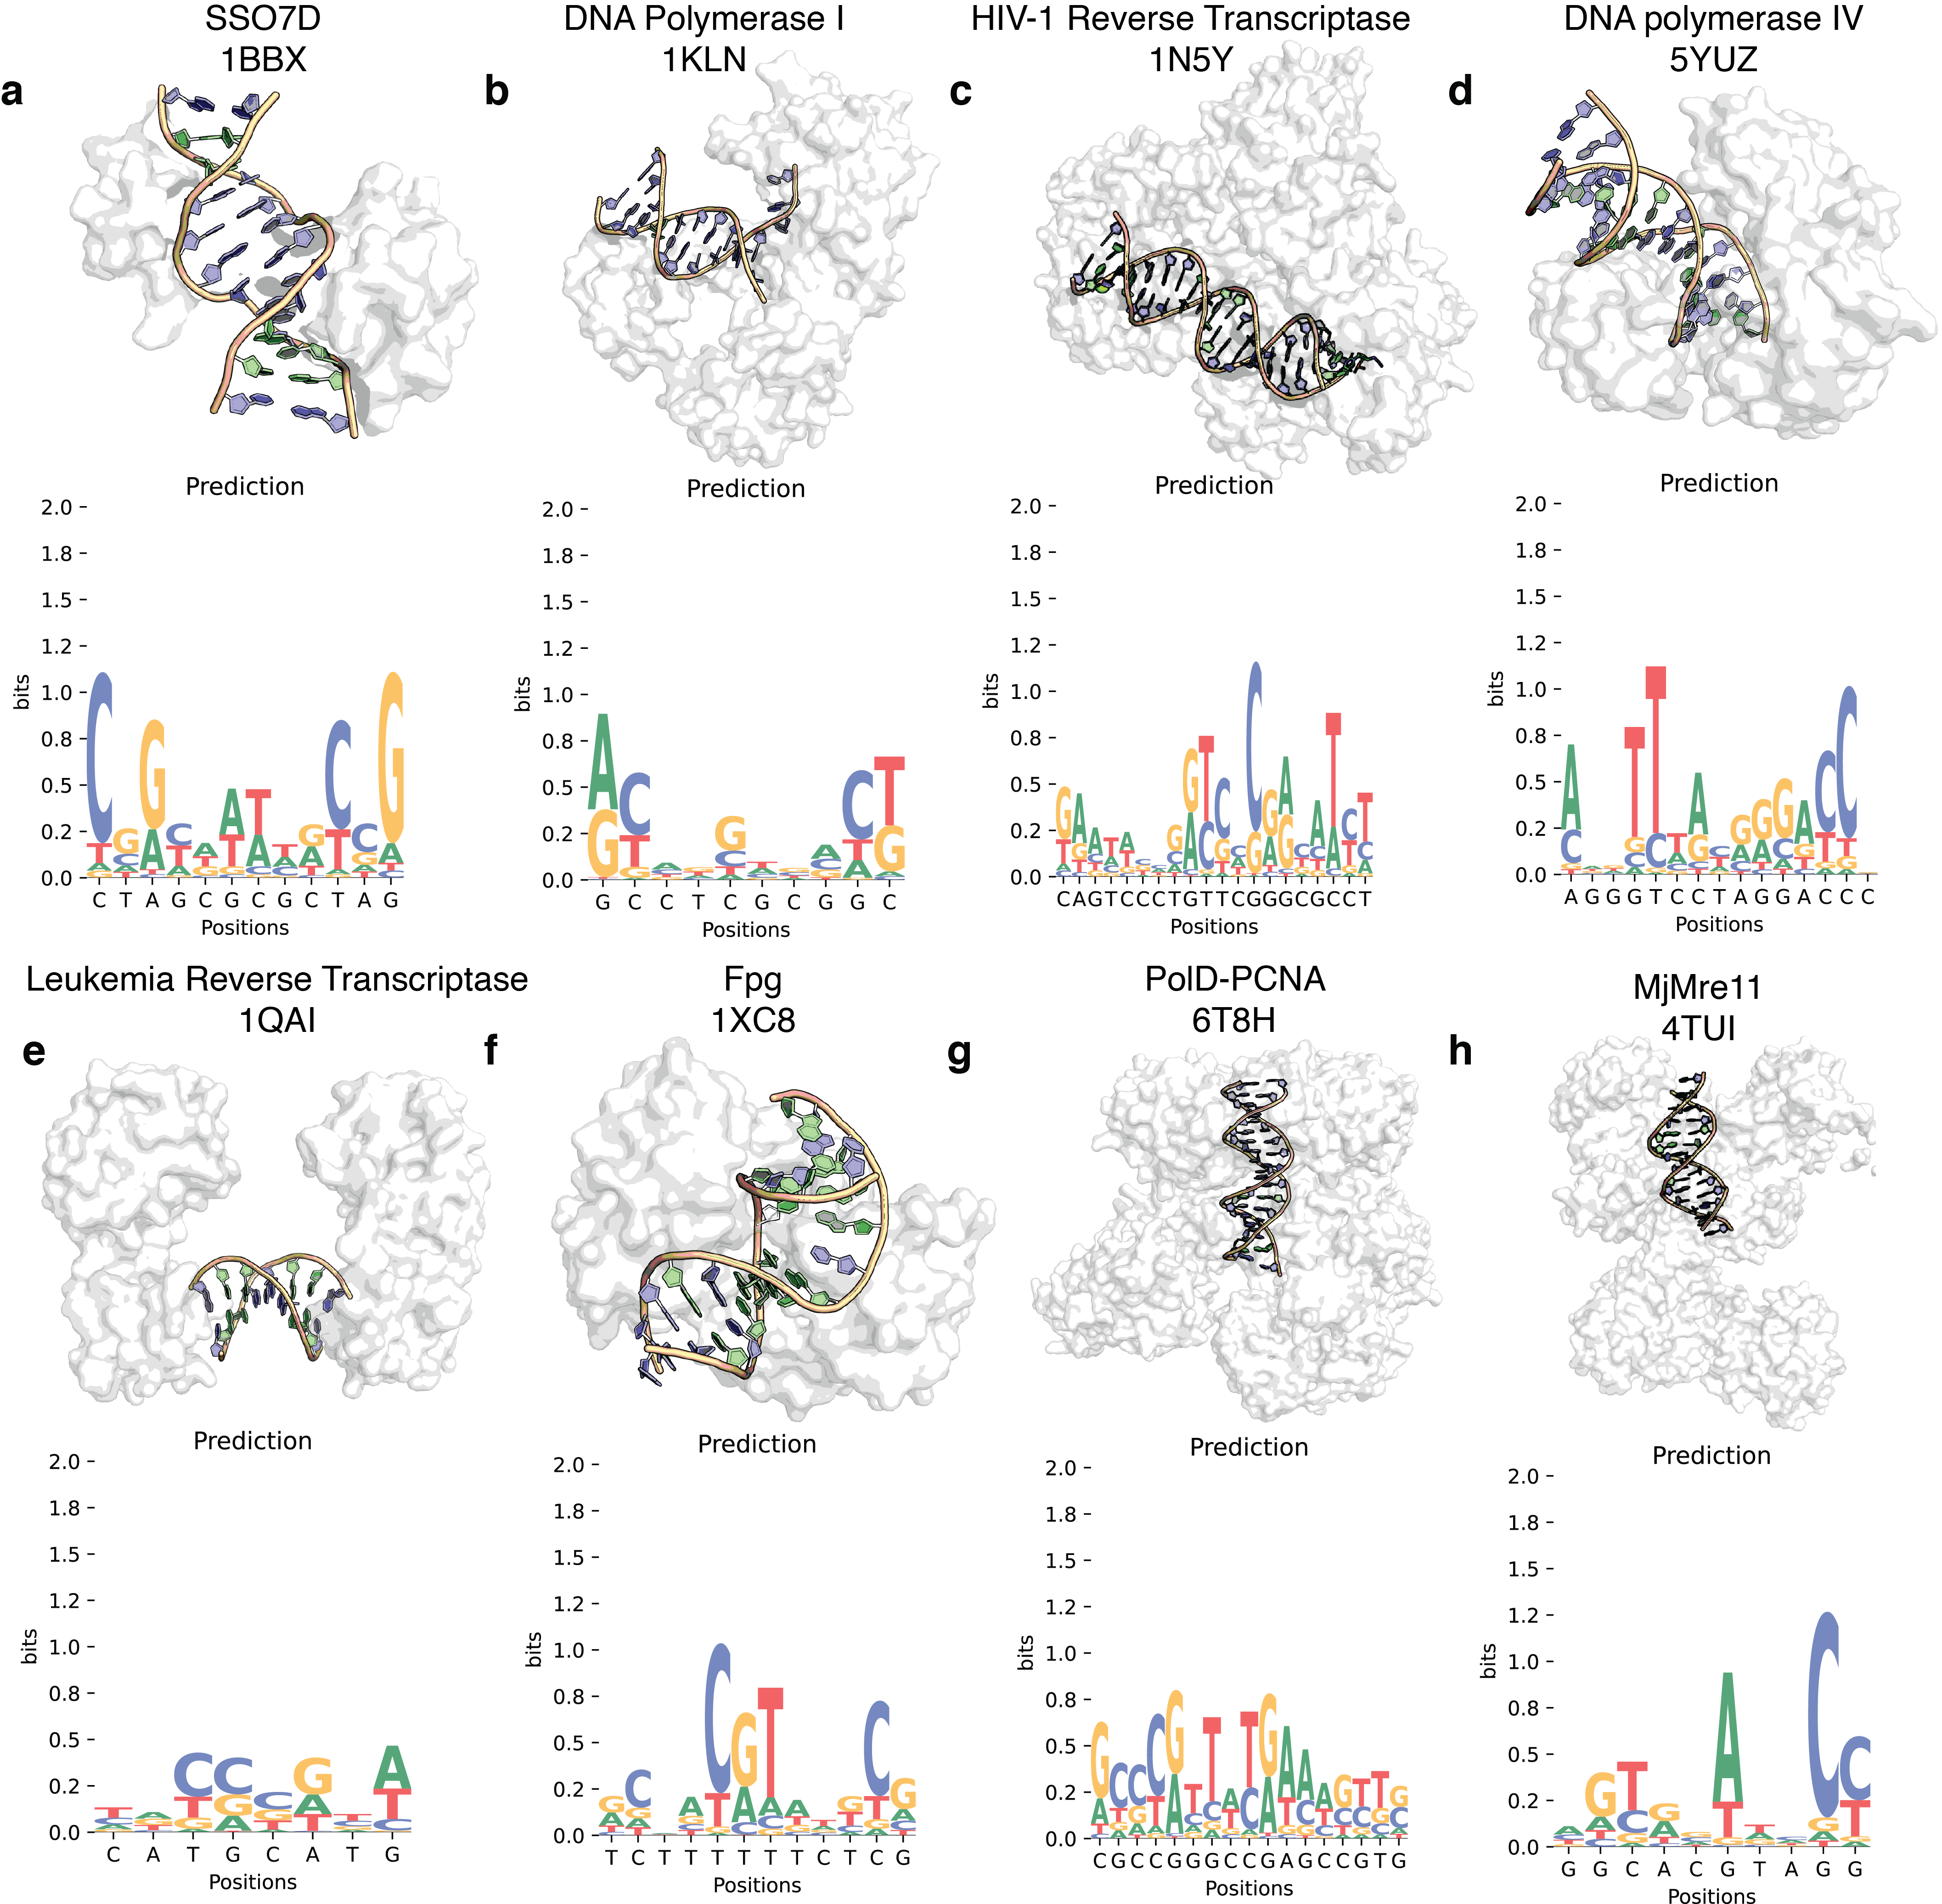
\includegraphics[width=\linewidth]{./pdnafigs/figS8.png}
 % archetecture.png: 1149x508 px, 72dpi, 40.53x17.92 cm, bb=0 0 1149 508
    \caption[Examples of continuous time prediction of ESC differentiation.]{\textbf{Examples of continuous time prediction of ESC differentiation.} Reconstruction (up to $t=6.8$) and future prediction (for $t>6.8$) for 4 example genes by a  latent ODE \citep{chen2018neural} trained on ESC data \citep{Klein2015} for 1000000 iterations, showing a good fit for the initial timepoints, but underfitting for the later timepoints.}
  \label{fig:pdnaS8}
\end{figure}
\end{center}

\begin{center}
\begin{figure}[H]
  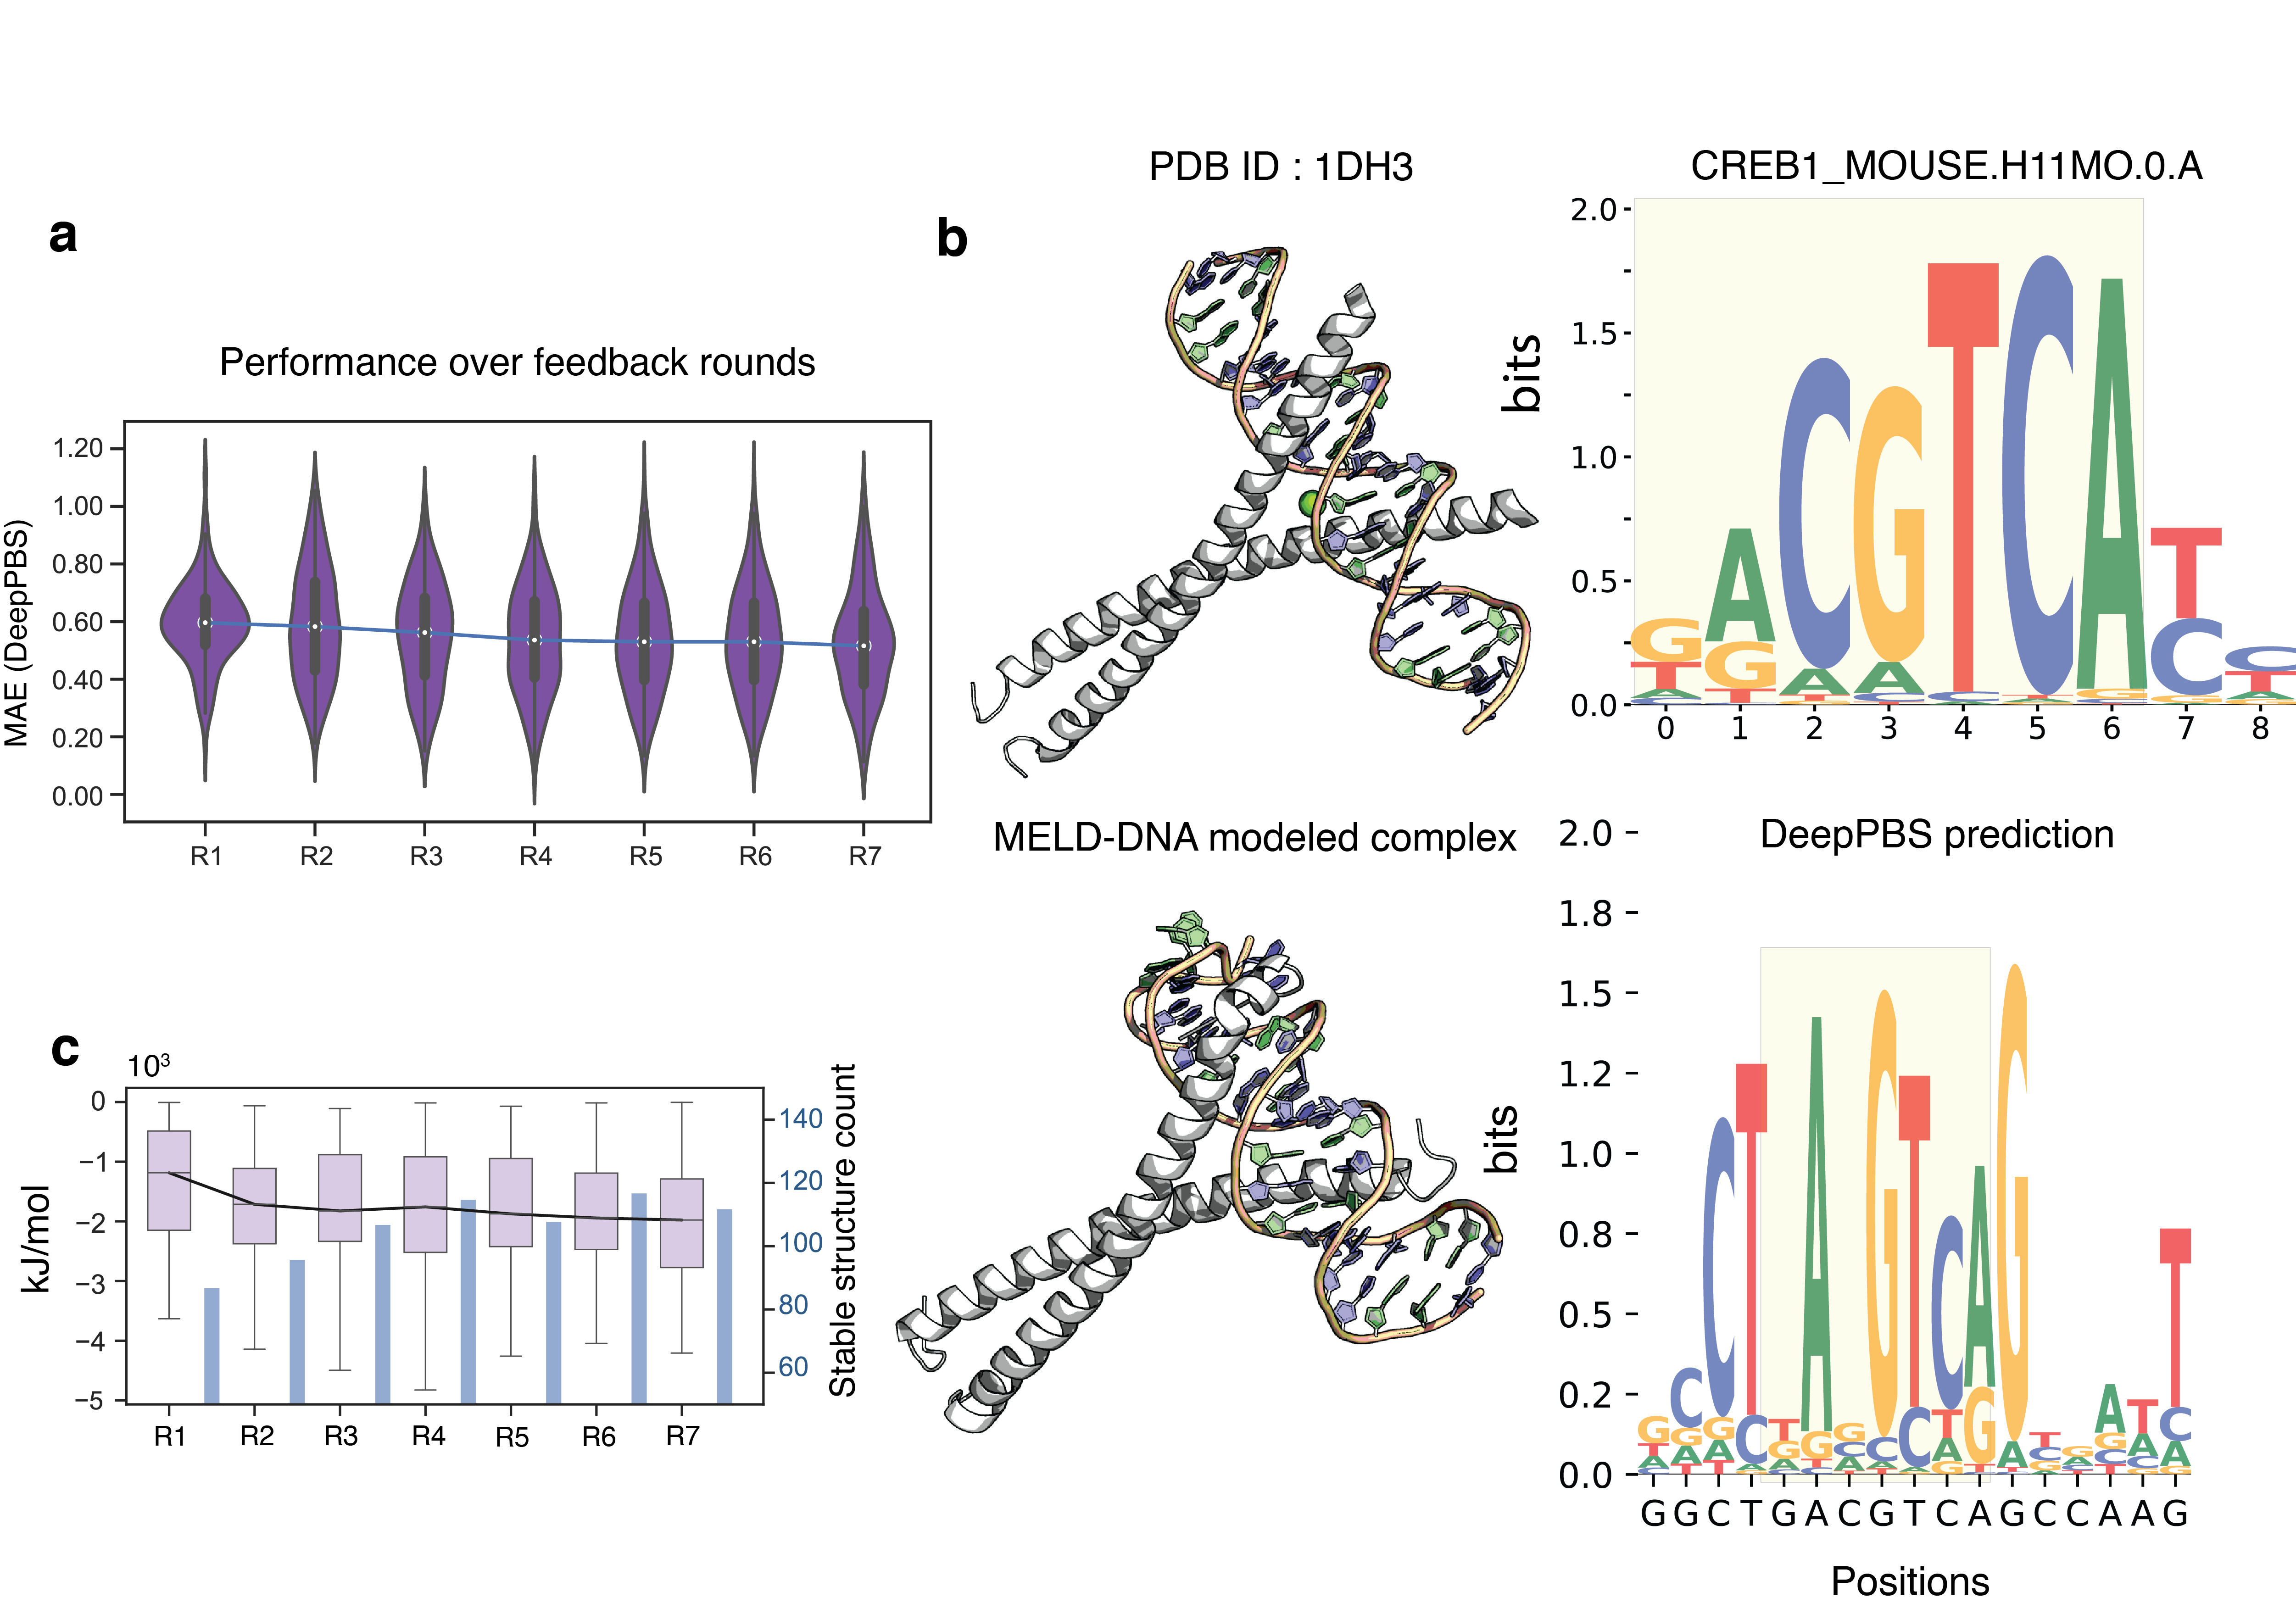
\includegraphics[width=\linewidth]{./pdnafigs/figS9.png}
 % archetecture.png: 1149x508 px, 72dpi, 40.53x17.92 cm, bb=0 0 1149 508
    \caption[Examples of continuous time prediction of ESC differentiation.]{\textbf{Examples of continuous time prediction of ESC differentiation.} Reconstruction (up to $t=6.8$) and future prediction (for $t>6.8$) for 4 example genes by a  latent ODE \citep{chen2018neural} trained on ESC data \citep{Klein2015} for 1000000 iterations, showing a good fit for the initial timepoints, but underfitting for the later timepoints.}
  \label{fig:pdnaS9}
\end{figure}
\end{center}

\begin{center}
\begin{figure}[H]
  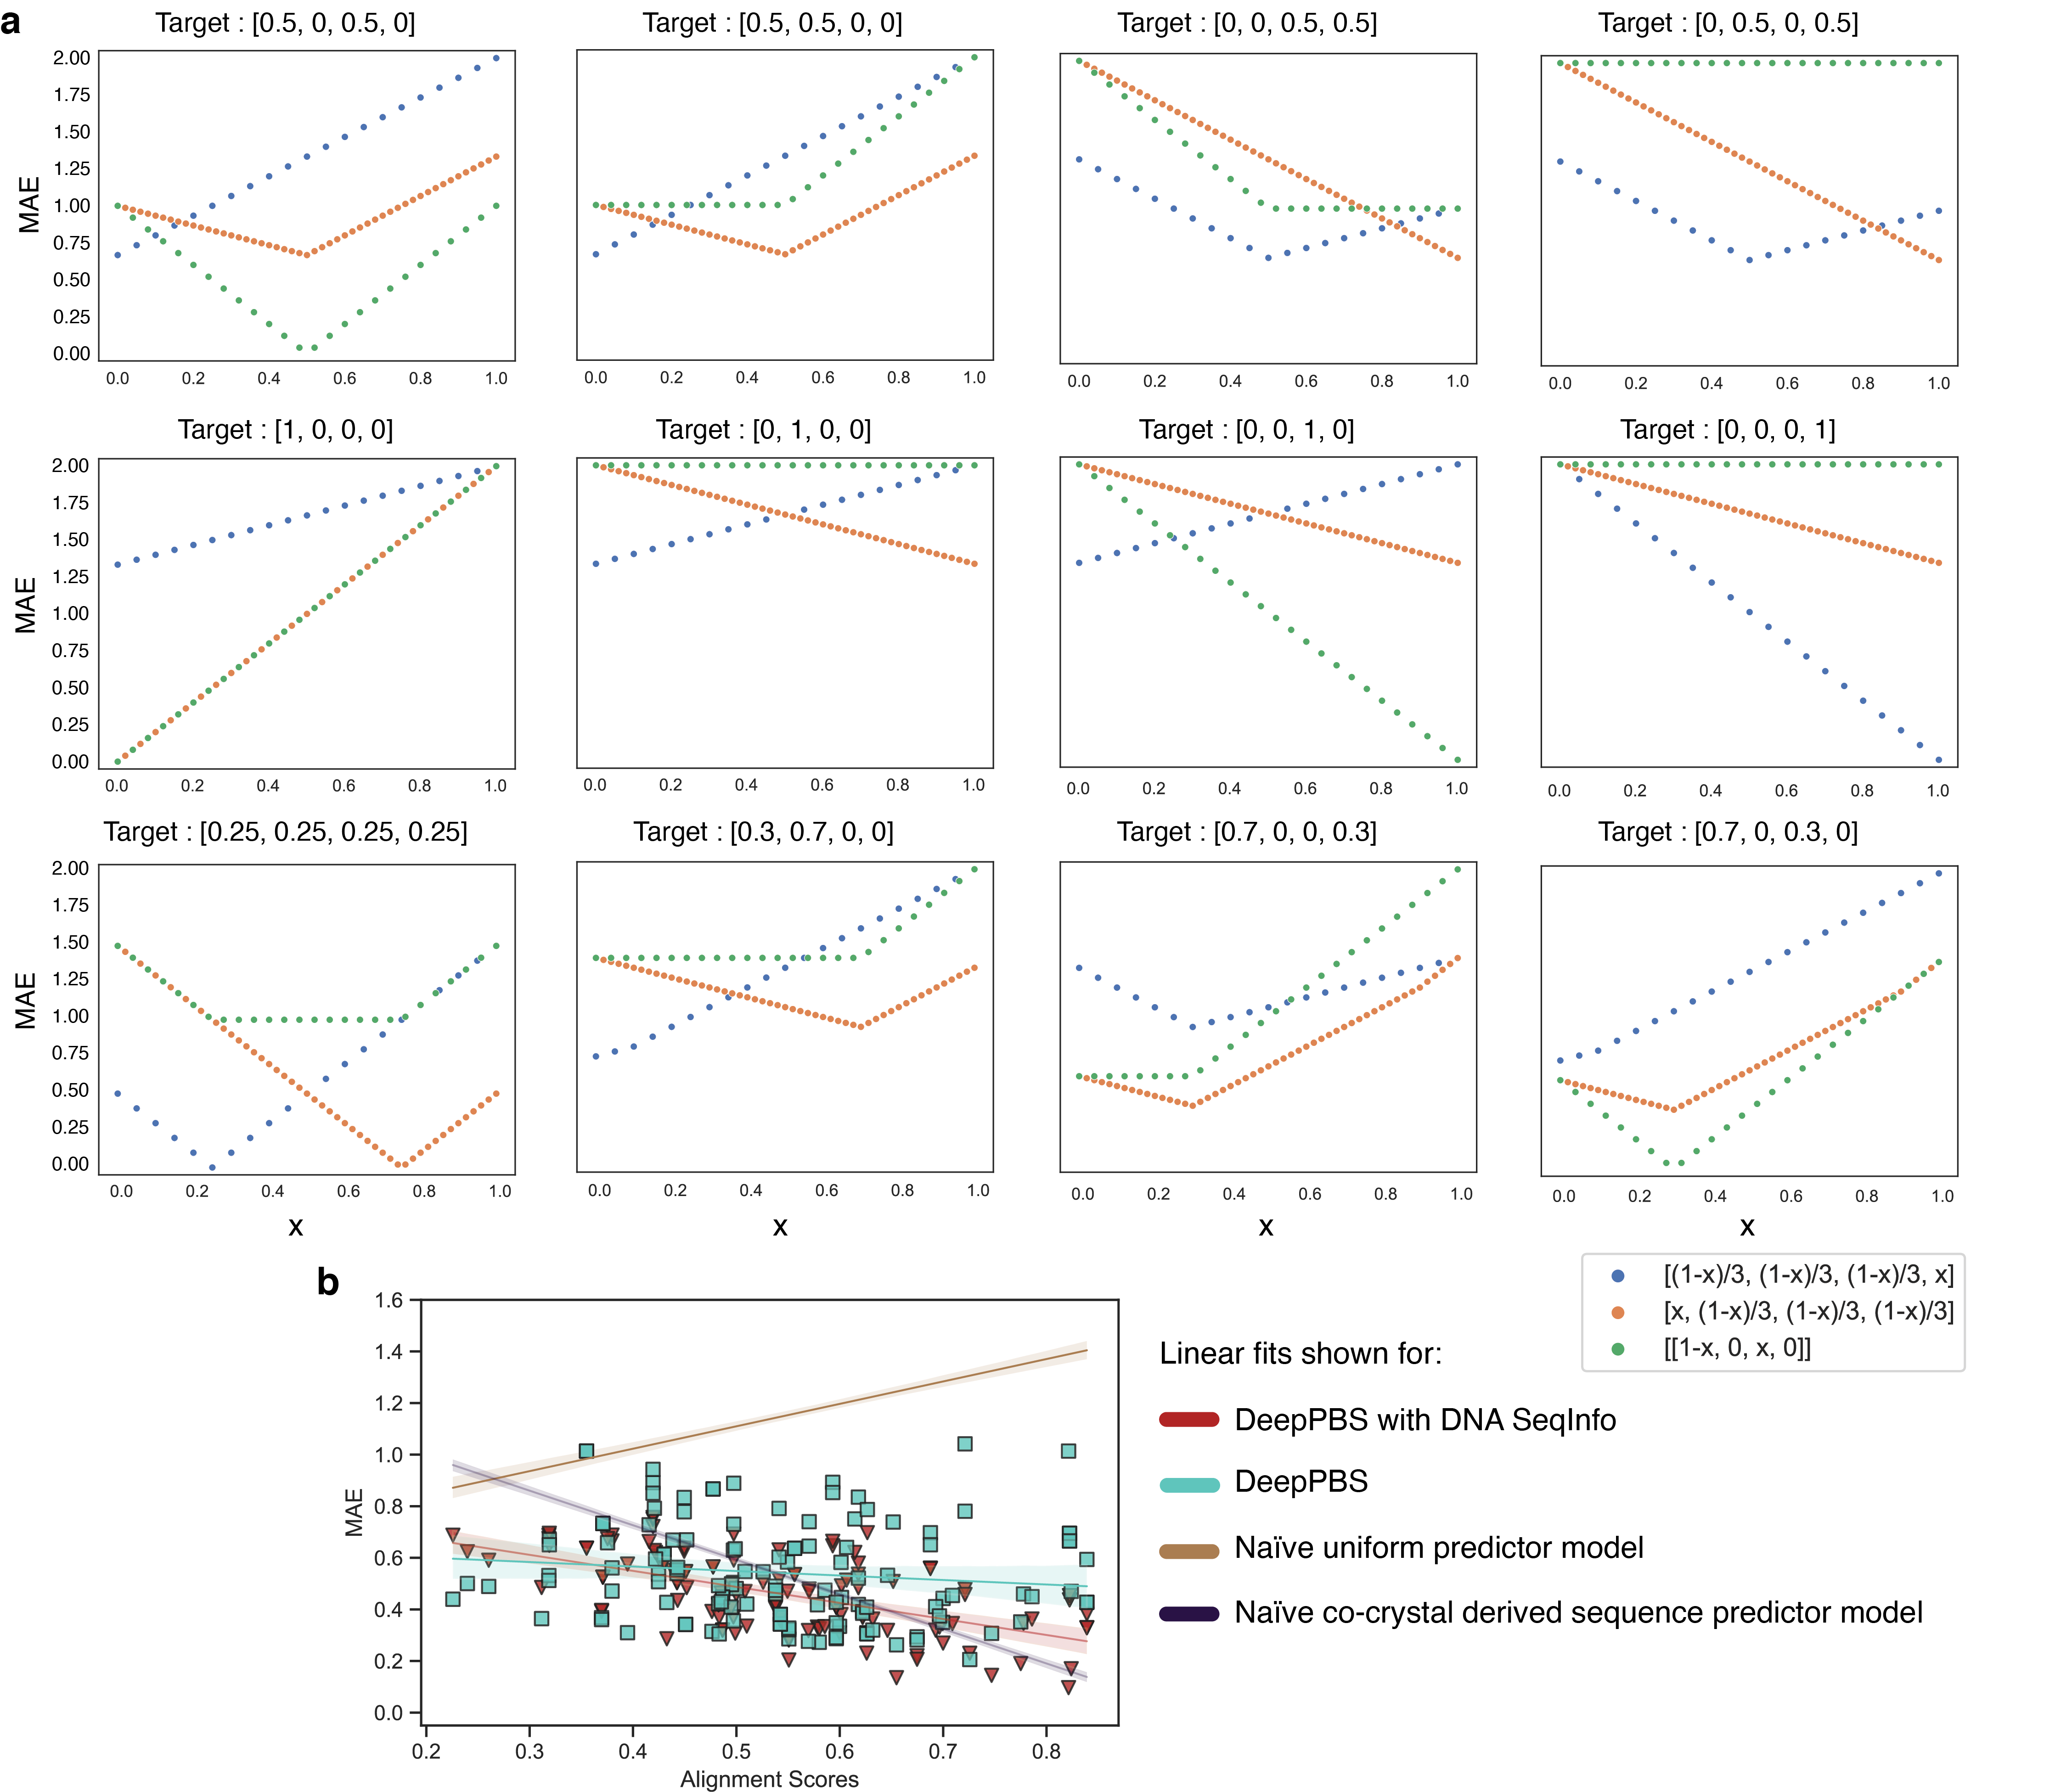
\includegraphics[width=\linewidth]{./pdnafigs/figS10.png}
 % archetecture.png: 1149x508 px, 72dpi, 40.53x17.92 cm, bb=0 0 1149 508
    \caption[Examples of continuous time prediction of ESC differentiation.]{\textbf{Examples of continuous time prediction of ESC differentiation.} Reconstruction (up to $t=6.8$) and future prediction (for $t>6.8$) for 4 example genes by a  latent ODE \citep{chen2018neural} trained on ESC data \citep{Klein2015} for 1000000 iterations, showing a good fit for the initial timepoints, but underfitting for the later timepoints.}
  \label{fig:pdnaS10}
\end{figure}
\end{center}

\begin{center}
\begin{figure}[H]
  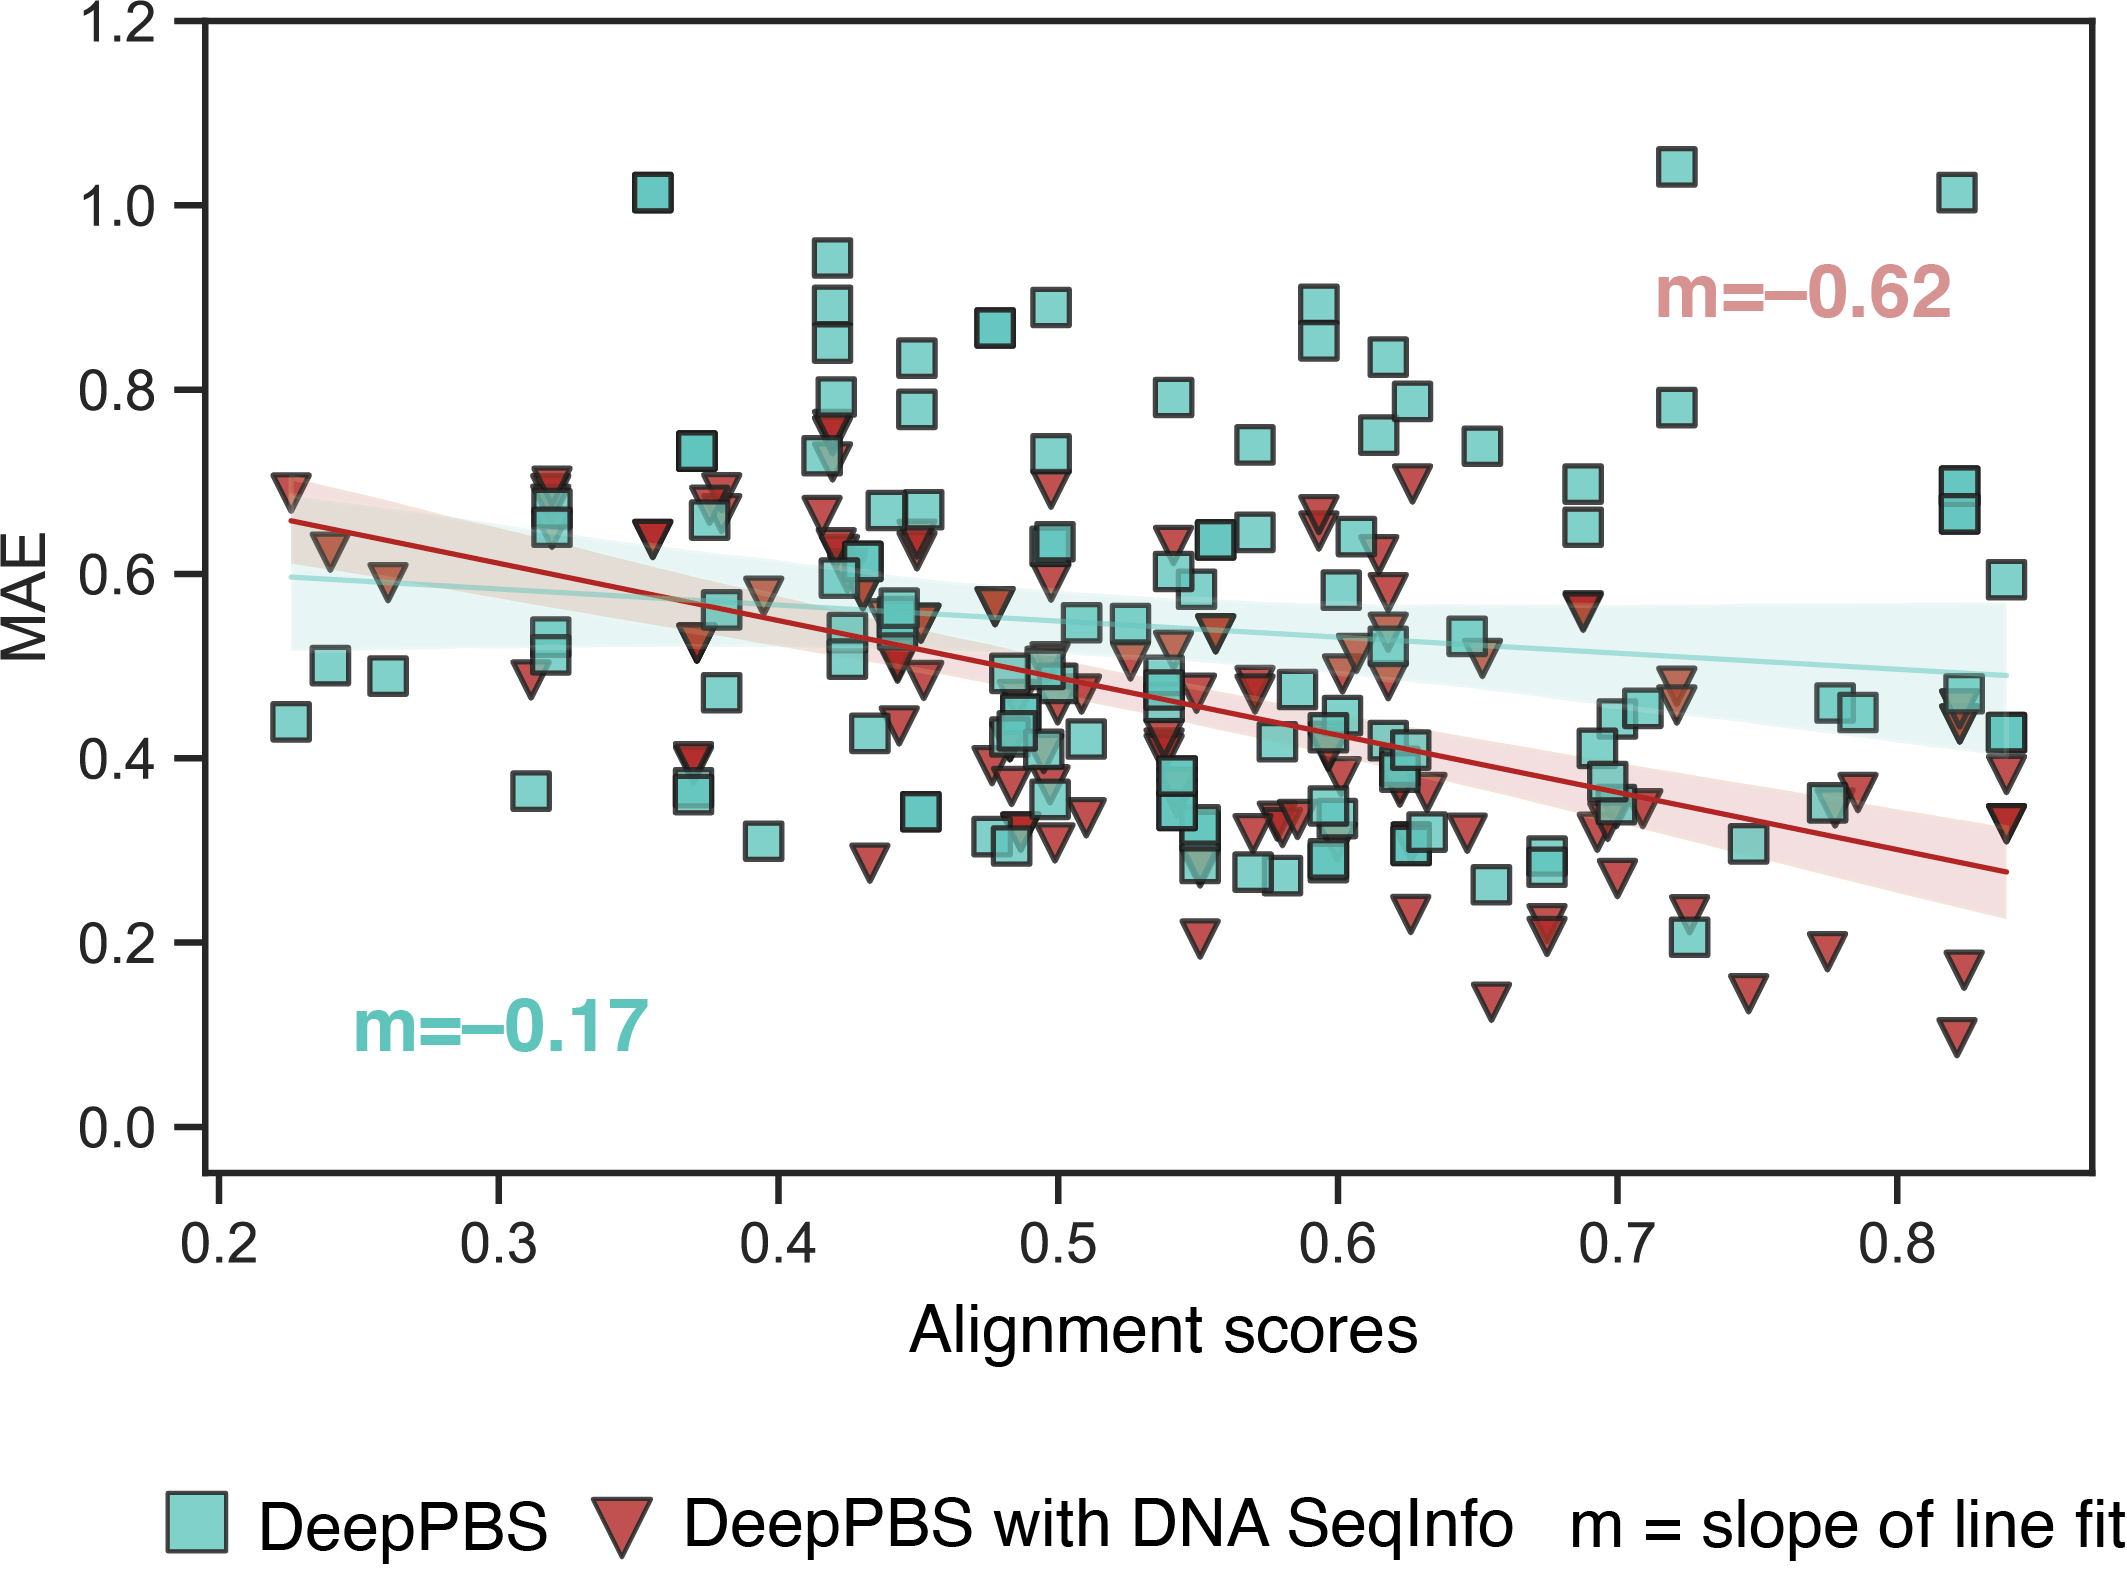
\includegraphics[width=\linewidth]{./pdnafigs/figS11.png}
 % archetecture.png: 1149x508 px, 72dpi, 40.53x17.92 cm, bb=0 0 1149 508
    \caption[Examples of continuous time prediction of ESC differentiation.]{\textbf{Examples of continuous time prediction of ESC differentiation.} Reconstruction (up to $t=6.8$) and future prediction (for $t>6.8$) for 4 example genes by a  latent ODE \citep{chen2018neural} trained on ESC data \citep{Klein2015} for 1000000 iterations, showing a good fit for the initial timepoints, but underfitting for the later timepoints.}
  \label{fig:pdnaS11}
\end{figure}
\end{center}

\begin{center}
\begin{figure}[H]
  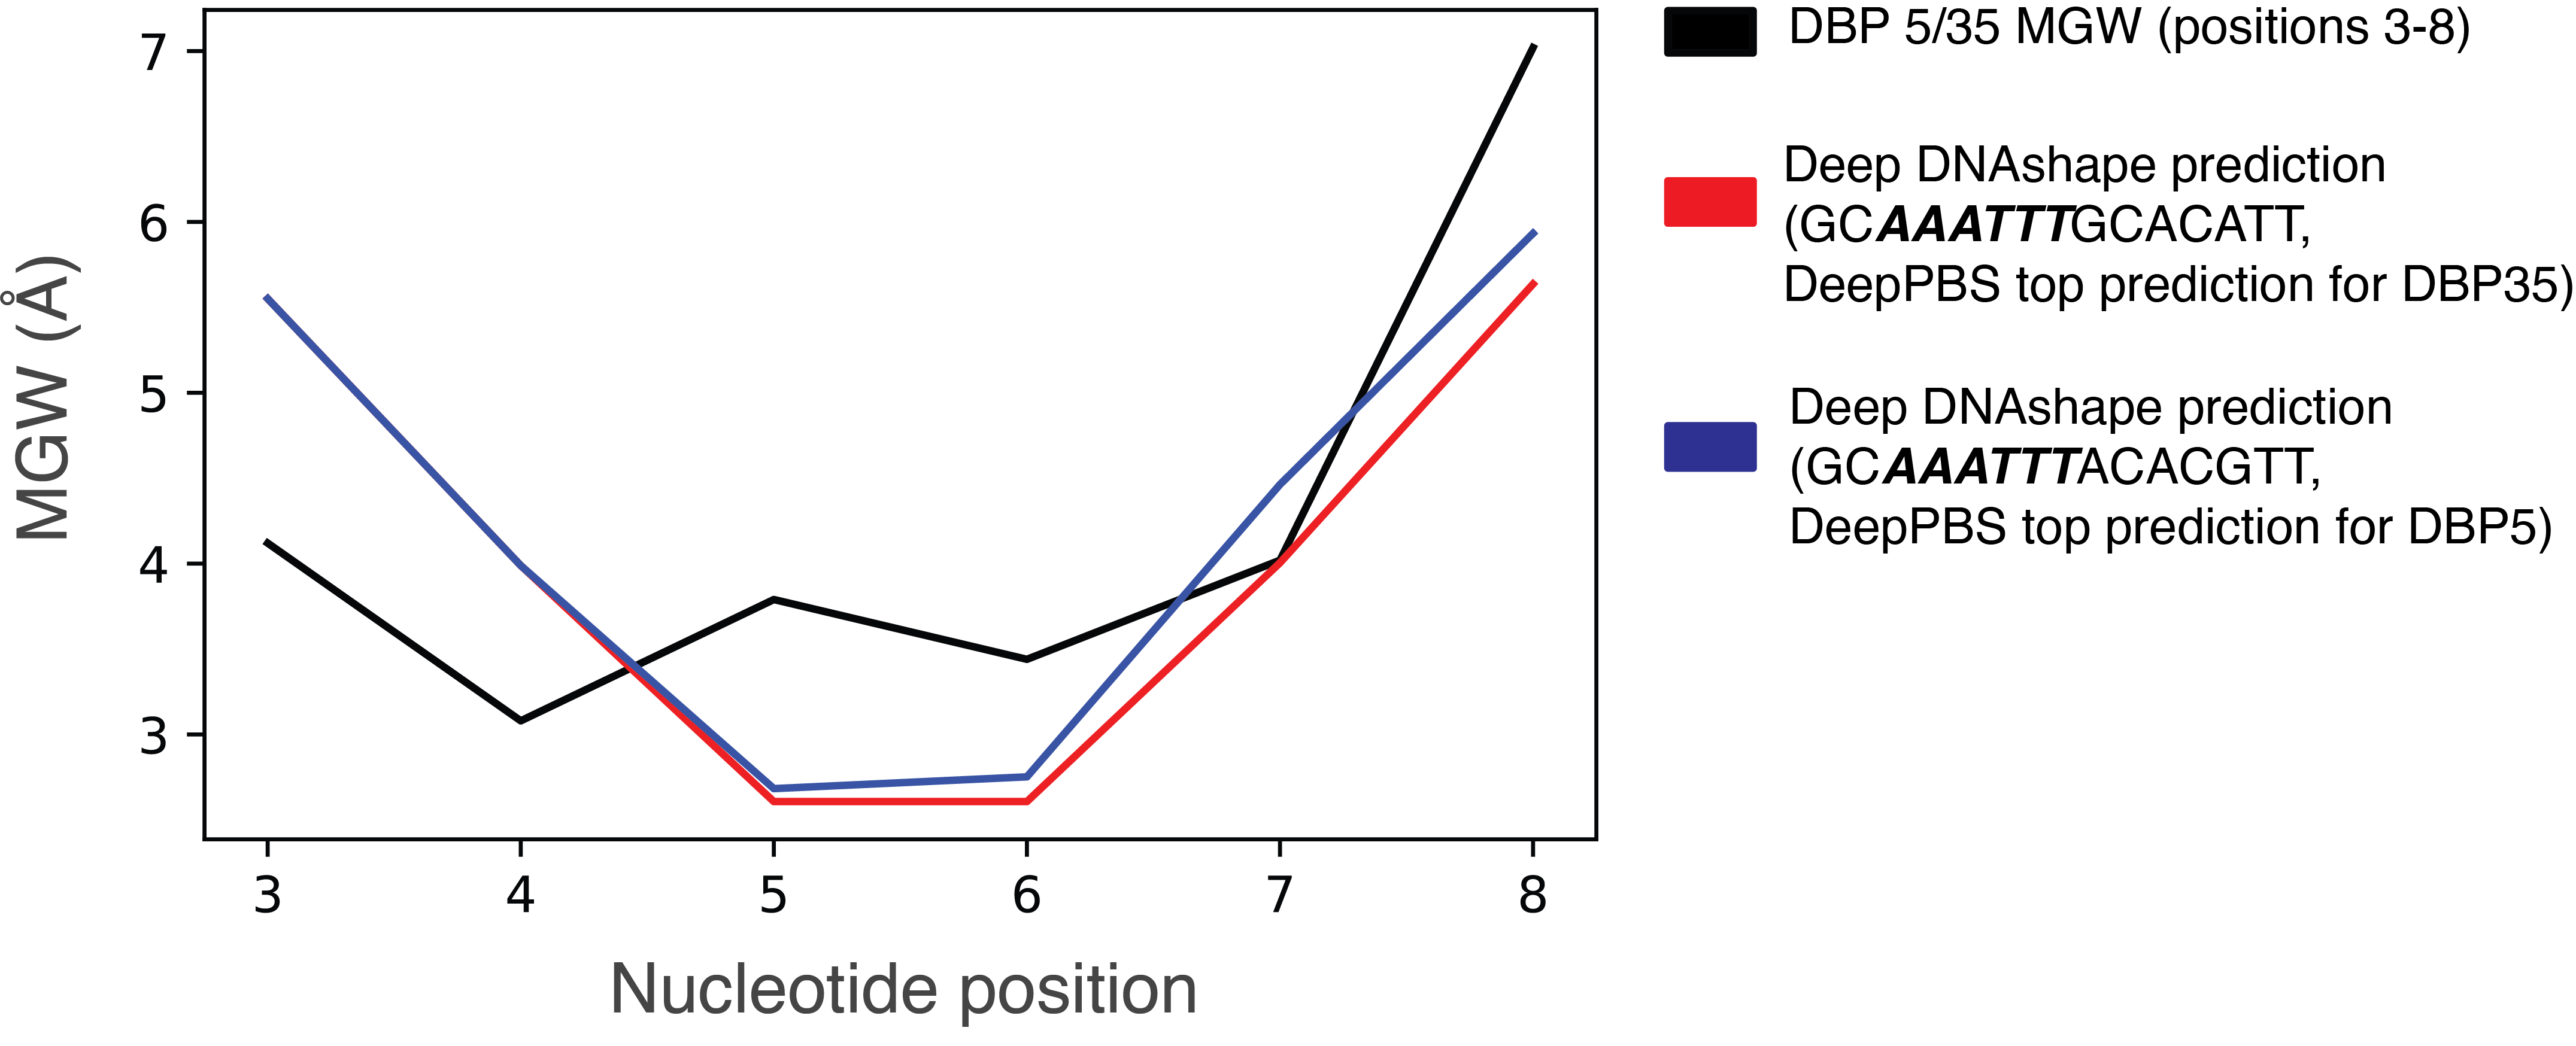
\includegraphics[width=\linewidth]{./pdnafigs/figS12.png}
 % archetecture.png: 1149x508 px, 72dpi, 40.53x17.92 cm, bb=0 0 1149 508
    \caption[Examples of continuous time prediction of ESC differentiation.]{\textbf{Examples of continuous time prediction of ESC differentiation.} Reconstruction (up to $t=6.8$) and future prediction (for $t>6.8$) for 4 example genes by a  latent ODE \citep{chen2018neural} trained on ESC data \citep{Klein2015} for 1000000 iterations, showing a good fit for the initial timepoints, but underfitting for the later timepoints.}
  \label{fig:pdnaS12}
\end{figure}
\end{center}
